\PassOptionsToPackage{unicode=true}{hyperref} % options for packages loaded elsewhere
\PassOptionsToPackage{hyphens}{url}
%
\documentclass[]{article}
\usepackage{lmodern}
\usepackage{amssymb,amsmath}
\usepackage{ifxetex,ifluatex}
\usepackage{fixltx2e} % provides \textsubscript
\ifnum 0\ifxetex 1\fi\ifluatex 1\fi=0 % if pdftex
  \usepackage[T1]{fontenc}
  \usepackage[utf8]{inputenc}
  \usepackage{textcomp} % provides euro and other symbols
\else % if luatex or xelatex
  \usepackage{unicode-math}
  \defaultfontfeatures{Ligatures=TeX,Scale=MatchLowercase}
\fi
% use upquote if available, for straight quotes in verbatim environments
\IfFileExists{upquote.sty}{\usepackage{upquote}}{}
% use microtype if available
\IfFileExists{microtype.sty}{%
\usepackage[]{microtype}
\UseMicrotypeSet[protrusion]{basicmath} % disable protrusion for tt fonts
}{}
\IfFileExists{parskip.sty}{%
\usepackage{parskip}
}{% else
\setlength{\parindent}{0pt}
\setlength{\parskip}{6pt plus 2pt minus 1pt}
}
\usepackage{hyperref}
\hypersetup{
            pdftitle={A White Noise Approach to Evolutionary Ecology},
            pdfauthor={Bob Week, Steve Krone, Scott L. Nuismer, Luke J. Harmon},
            pdfborder={0 0 0},
            breaklinks=true}
\urlstyle{same}  % don't use monospace font for urls
\usepackage[margin=1in]{geometry}
\usepackage{graphicx,grffile}
\makeatletter
\def\maxwidth{\ifdim\Gin@nat@width>\linewidth\linewidth\else\Gin@nat@width\fi}
\def\maxheight{\ifdim\Gin@nat@height>\textheight\textheight\else\Gin@nat@height\fi}
\makeatother
% Scale images if necessary, so that they will not overflow the page
% margins by default, and it is still possible to overwrite the defaults
% using explicit options in \includegraphics[width, height, ...]{}
\setkeys{Gin}{width=\maxwidth,height=\maxheight,keepaspectratio}
\setlength{\emergencystretch}{3em}  % prevent overfull lines
\providecommand{\tightlist}{%
  \setlength{\itemsep}{0pt}\setlength{\parskip}{0pt}}
\setcounter{secnumdepth}{5}
% Redefines (sub)paragraphs to behave more like sections
\ifx\paragraph\undefined\else
\let\oldparagraph\paragraph
\renewcommand{\paragraph}[1]{\oldparagraph{#1}\mbox{}}
\fi
\ifx\subparagraph\undefined\else
\let\oldsubparagraph\subparagraph
\renewcommand{\subparagraph}[1]{\oldsubparagraph{#1}\mbox{}}
\fi

% set default figure placement to htbp
\makeatletter
\def\fps@figure{htbp}
\makeatother

\usepackage{mathtools}
\usepackage{mathrsfs}
\usepackage{hyperref}
\usepackage[left]{lineno}
\usepackage{amsmath}
\linenumbers
\usepackage{float}
\usepackage{flafter}

\title{A White Noise Approach to Evolutionary Ecology}
\author{Bob Week, Steve Krone, Scott L. Nuismer, Luke J. Harmon}
\date{3/1/2020}

\begin{document}
\maketitle
\begin{abstract}
We derive the dynamics of the distribution of a quantitative character
and the abundance of a biological population from a stochastic partial
differential equation driven by space-time white noise. In the process
we develop a useful set of heuristics to operationalize the powerful,
but abstract theory of white noise and measure-valued stochastic
processes. This approach allows us to compute the full implications of
demographic stochasticity on phenotypic distributions and abundances of
populations. We demonstrate the utility of our approach by deriving a
quantitative genetic model of diffuse coevolution mediated by
exploitative competition for a continuum of resources. Other than trait
and abundance distributions, this model predicts interaction networks
parameterized by rates of interactions, competition coefficients, and
selection gradients. We briefly investigate the relationship between
selection gradients and competition coefficients. This illustrative
investigation suggests selection gradients can be either positively or
negatively correlated with competition coefficients depending on the
ratio of interspecific trait variation to intraspecific trait variation.
Hence, this approach contributes to the development of a synthetic
theory of evolutionary ecology by formalizing first principle
derivations of stochastic models that underlie rigorous investigations
of the relationship between feedbacks of biological processes and the
patterns of diversity they produce.
\end{abstract}

\hypertarget{introduction}{%
\section{Introduction}\label{introduction}}

Our goal in this manuscript is to develop a rigorous, but accessible
approach to synthesize the stochastic dynamics of abundance, mean trait
and heritable variation in biological populations for the study of
theoretical evolutionary ecology. A primary aim of theoretical
evolutionary ecology is the development of mathematical approaches to
describe the evolution of populations and their interactions with both
the biotic and abiotic environments in which they are embedded. Given
this consideration, a natural scope for such an approach centers on
quantifying the abundance dynamics of populations and the evolution of
traits mediating their interactions as functions of relevant abiotic
factors. Although taking into account abundance, phenotype and
environment provides the basis for a partial understanding of the
complex nature of biological communities, a deeper understanding must
account for the effects of dispersal and the phylogeographic history of
interacting lineages (Kraft et al. 2007; Hickerson et al. 2010; Manceau,
Lambert, and Morlon 2016; McPeek 2017) along with the genetic basis of
ecologically relevant traits (Conner 2004; Fussman, Loreau, and Abrams
2007) and feedbacks between populations and the biogeochemical cycles
they ultimately depend on (Loreau 2010; Ågren and Andersson 2012). It is
therefore ideal that the development of any such mathematical approach
anticipates extensions to account for these important factors shaping
ecological communities, especially as empirical and conceptual work in
these directions continues to grow (Abdala-Roberts and Mooney 2014;
Kölzsch et al. 2015; Crutsinger 2015; Fitzpatrick et al. 2015, 2017;
Marx et al. 2017; Rudman et al. 2017; Skovmand et al. 2018; Nuland et
al. 2019; Harmon et al. 2019). Furthermore, the approach would benefit
from a stochastic component to capture the chance nature of biological
reality (Lande, Engen, and SÆther 2003; Meester et al. 2018; Mubayi et
al. 2019) and serve as a basis for the construction of statistical
methods that measure evolutionary and ecological processes occuring in
the wild. Such methods will tether theory to reality and allow for
rigorous tests of hypotheses on the structure and behavior of ecological
communities. In this paper we introduce a framework that establishes a
formal connection between the continuous-time dynamics of abundance and
quantitative traits in stochastically evolving populations. We then
demonstrate the utility of our framework through the derivation and
analysis of a model of diffuse coevolution and discuss how it can be
extended to account for the details mentioned above.

Current theoretical approaches to synthesize evolution and ecology have
capitalized on the fact that biological fitness plays a key role in
determining both sets of dynamics. While correlation of fitness and
genotype is the basis of evolution by natural selection, the mean
fitness across all individuals in a population determines the growth,
stasis or decline of abundance. In section \ref{deterministic} we review
the mathematical formalization of this connection, which has been
established in the contexts of population genetics (Crow and Kimura
1970; Roughgarden 1979), evolutionary game theory (Hofbauer and Sigmund
1998; Nowak 2006; Lion 2018), quantitative genetics (Lande 1982; Doebeli
1996; Lion 2018) and a unifying framework for these three distinct
approaches to evolutionary theory (Champagnat, Ferrière, and Méléard
2006) which includes our approach as a special case. We note here there
are two primary differences between our aims and those of Champagnat,
Ferrière, and Méléard (2006). First, instead of developing a unifying
approach to evolutionary theory, we focus on developing a stochastic
synthesis of population dynamics and quantitative genetics including
specific expressions for the dynamics of abundance, mean trait and
additive genetic variance. Second, although Champagnat, Ferrière, and
Méléard (2006) provide rigorous proofs of results relevant to our
approach, they do not communicate the nessecary tools we make use of for
deriving the dynamics of abundance, mean trait and additive genetic
variance. We aim to communicate these tools to a wide audience by
providing an intuitive, yet accurate treatment of white noise and
associated heuristics useful for deriving new stochastic models of
evolutionary ecology.

Reviewing the above accomplishments reveals a beautiful synthesis of
evolution and population ecology. However, it also reveals a gap in
theoretical approaches to incorporate the intrinsically random nature of
populations. Specifically, in theoretical quantitative genetics the
derivation of a population's response to random genetic drift is derived
in discrete time under the assumption of constant effective population
size using arguments based on properties of random samples (Lande 1976).
Though this approach conveniently mimics the formalism provided by the
Wright-Fisher model of population genetics, real population sizes
fluctuate over time. Furthermore, since these fluctuations are
themselves stochastic, it seems natural to derive expressions for the
evolutionary response to demographic stochasticity and consider how the
results relate to characterizations of random genetic drift. This can be
done in continuous time for population genetic models without too much
technical overhead, assuming a finite number of alleles (Lande, Engen,
and Sæther 2009; Parsons, Quince, and Plotkin 2010; Gomulkiewicz, Krone,
and Remien 2017). However, for populations with a continuum of types,
such as a quantitative trait, finding a formal approach to derive the
evolutionary response to demographic stochasticity has remained a vexing
mathematical challenge. Previous work integrating stochastic processes
with quantitative genetic models have profited from the simplifying
assumption that phenotypic and genetic variances remain constant over
time, yeilding analytical approximations for the joint dynamics of
abundance and the mean of a quantitative trait (Engen, Lande, and Sæther
2013). These results not only ignore the evolution genetic variance, but
they focus on environmental stochasticity and assume sufficiently large
populations so that demographic stochasticity is negligible. Here we
account for both demographic stochasticity and the evolution of additive
genetic variance by combining the calculus of white noise with results
on rescaled limits of branching Brownian motion processes (BBM) and
stochastic partial differential equations (SPDE), which are stochastic
analogs of deterministic partial differential equations (PDE). Our goal
has two components: 1) Establish a novel synthetic approach to
theoretical evolutionary ecology that provides a formal connection
between demographic stochasticity and random genetic drift in the
context of quantitative traits. 2) Communicate some useful properties of
space-time white noise, BBM and SPDE to as wide of audience as possible.
With this goal in mind we will not provide a rigorous treatment of any
of these deep subjects. Instead, we introduce a set of heuristics that
only require the basic concepts of Reimann integration, partial
differentiation and some exposure to Brownian motion and stochastic
ordinary differential equations (SDE). For a concise introduction to SDE
and Brownian motion, we recommend the primer by Evans (2014). Rigorous
treatments of SPDE and rescaled limits of BBM can be found in Walsh
(1986) and Dawson (1993) respectively.

Through accomplishing these goals this work yields five main results.
Firstly, we develop a concise, but accurate approach for understanding
SPDE and provide heuristics to empower mathematical evolutionary
ecologists to derive novel models that relax key assumptions commonly
made in combining models of evolutionary and abundance dynamics. Second,
we formally derive general SDE that express the joint dynamics of
abundance, mean trait and additive genetic variance for populations
exhibiting a wide range of potential phenotypic distributions. Third, we
simplify these SDE by approximating the abundance density of phenotypes
with a Gaussian curve and integrate the results with a model of
imperfect inheritance to find formula that generalize classical
quantitative genetic expressions. This includes an expression for
additive genetic variance analogous to the expression for the response
in mean phenotype found by Lande (1976). Fourth, following classical
niche theory we provide a rigorous mechanistic derivation of fitness for
populations experiencing resource competition and abiotic stabilizing
selection using diffusion limits of measure-valued branching processes.
This calculation provides a demonstration for performing such diffusion
limits that can be applied in other contexts. Fifth, we explore
implications of the resulting model of diffuse coevolution by
investigating the relationship between selection gradients and
competition coefficients.

We now summarize the basic structure of the paper. To provide motivation
for the stochastic equations developed later and background for our
model of coevolution, we begin with \S\ref{deterministic} by briefly
summarizing derivations of deterministic dynamics of biological
populations. Starting with a PDE (which we refer to as the Deterministic
Asexual Gaussian allelic model with Abundance dynamics, abbreviated
DAGA), we arrive at a general set of ordinary differential equations
modelling the dynamics of abundance, trait mean and trait variance. We
discuss the relationship between DAGA and previous models of phenotypic
evolution that have been employed in theoretical quantitative genetics.
Noting that a natural stochastic generalization of DAGA has been
previously derived, we find a path to derive SDE describing the
evolutionary response to demographic stochasticity. We accomplish this
in \S\ref{wnc} by discussing how a diffusion limit of a spatially
structured branching process (i.e., a measure-valued branching process)
leads to the natural SPDE appropriate for our study. We refer to this
SPDE as the Stochastic Asexual Gaussian allelic model with Abundance
dynamics (abbreviated SAGA). The diffusion limit in turn provides a
rigorous method for constructing fitness functions used in models of
evolutionary ecology. However, before we discuss measure-valued braching
processes and their diffusion limits, we find it necessary to review
some fundamental results on the calculus of white noise and introducing
a set of mathematical tools based on these results. In \S\ref{wnc} and
SM \S\ref{SDE_DERIV} we employ these tools to derive a system of SDE
generalizing our deterministic results to account for demographic
stochasticity. We find that the effect of demographic stochasticity on
the evolution of mean trait and phenotypic variance characterizes the
process of random genetic drift in continuous time. However, although
biologically insightful, these equations remain difficult to analyze and
implement numerically. In \S\ref{equations} we use an assumption of
normally distributed trait values to simplify these expressions into
formulae that are much easier to work with. We then account for the
constraint of adaptive evolution on the amount of heritable variation in
a population by extending these results via a model of imperfect
inheritance. The resulting equations coincide with classical results in
quantitative genetics as a special case. In \S\ref{coev} we combine the
derived equations of population dynamics with classical niche theory to
formulate a model of coevolution across a guild of \(S\) species
participating in exploitative competition along a common resource
continuum. In SM \S\ref{diffuse} we apply a classical theorem on
rescaled limits of BBM that allow for ecological interactions to provide
a rigorous derivation. To gain biological insight, in \S\ref{dynamics}
we numerically integrate our model of coevolution for \(S=100\) species,
tracking the dynamics of traits and abundances under scenarios of weak
and strong competition. We include an account of the natural history of
the simulated system and discuss the significance of demographic
stochasticity for structuring ecological communities. In \S\ref{ecoevo}
we provide expressions for selection gradients and competition
coefficients implied by our model and use these expressions to
investigate the relationship between the degree of competition and
strength of coevolution. Finally, \S\ref{conclusion} concludes with a
summary of accomplishments, a few remarks on the limits of this approach
and future directions to incorporate more explicitly the effects of
small populations, the genetic architecture of quantitative traits,
feedbacks with ecosystem processes and the macroevolutionary history of
interacting lineages.

\hypertarget{the-framework}{%
\section{The framework}\label{the-framework}}

At the core of our approach is a stochastic analog of the replicator
equation with mutation in continuous time and phenotypic space (Taylor
and Jonker 1978; Schuster and Sigmund 1983). From this stochastic
replicator-mutator equation we derive a system of SDE for the dynamics
of abundance, mean trait and additive genetic variance of a population.
Hence, our approach develops a quantitative genetic theory of
evolutionary ecology. A popular alternative to quantitative genetics is
the theory of adaptive dynamics. As demonstrated by Page and Nowak
(2002) and Champagnat, Ferrière, and Méléard (2006), the canonical
equation of adaptive dynamics can be derived from the replicator-mutator
equation. Thus, one could start from the atomic roots of our approach
and pursue a stochastic adaptive dynamic theory instead. We choose the
former in anticipation of an extension of our approach that explicitly
models the genetic details of populations.

In this section we review the derivations of the replicator-mutator
equation and trait dynamics from abundance dynamics and extend these
formulae along with related results to the stochastic case. The results
established in this section provide the framework from which larger
scale ecological stuctures, such as species abundance distributions and
interaction networks, can be computed.

\hypertarget{deterministic-dynamics}{%
\subsection{\texorpdfstring{Deterministic dynamics
\label{deterministic}}{Deterministic dynamics }}\label{deterministic-dynamics}}

Our review begins by considering the dynamics of an asexually
reproducing population in a homogeneous environment. For simplicity, we
first assume individuals are haploid and carry one of \(K\) alleles each
with a different fitness expressed as growth rate before introducing a
model involving a quantitative trait. Under these assumptions, the
derivation of the evolution of allele frequencies due to natural
selection can be derived from expressions of exponential growth. This,
and a few related approaches, have been provided by Crow and Kimura
(1970, \S 5.3). Specifically, denoting \(\nu_i\) the abundance of
individuals with allele \(i\) and \(m_i\) the growth rate of allele
\(i\) (called the Malthusian parameter in Crow and Kimura 1970), we have
\begin{equation}\label{first}
\frac{d\nu_i}{dt}=m_i\nu_i.
\end{equation} Starting from this model, we get the total abundance of
the population as \(N=\sum_{i=1}^K\nu_i\), the frequency of allele \(i\)
as \(p_i=\nu_i/N\) and the mean fitness of the population as
\(\bar m=\sum_{i=1}^Kp_im_i\). Hence, we can employ some elementary
calculus to derive the dynamics of abundance \(dN/dt\) and the dynamics
of allele frequencies \(dp_1/dt,\dots,dp_K/dt\) as \begin{equation}
\frac{dN}{dt}=\sum_{i=1}^K\nu_im_i=N\sum_{i=1}^Kp_im_i=\bar mN,
\end{equation} \begin{equation}\label{popgen}
\frac{dp_i}{dt}=\frac{d}{dt}\frac{\nu_i}{N}=\frac{1}{N^2}\left(N\frac{d\nu_i}{dt}-\frac{dN}{dt}\nu_i\right)
=\frac{1}{N}\left(m_i\nu_i-\bar m Np_i\right)=(m_i-\bar m)p_i.
\end{equation} Two important observations of these equations include 1)
mean fitness \(\bar m\) determines the abundance dynamics of the entire
population and 2) allele \(i\) will increase (decrease) in frequency if
\(m_i>\bar m\) (\(<\bar m\)). Equation (\ref{popgen}) is known in the
field of evolutionary game theory as the replicator equation (Hofbauer
and Sigmund 1998; Nowak 2006; Lion 2018; Taylor and Jonker 1978;
Schuster and Sigmund 1983). Instead of being explicitly focused on
alleles, the replicator equation describes the fluctuations of relative
abundances of various \emph{types} in a population in terms of the vital
rates of each type. Using a matrix of transition rates between differing
types, it is straight-forward to extend the replicator equation to
include mutation, which is known as the replicator-mutator equation
(Nowak 2006).

Inspired by equations (\ref{first})-(\ref{popgen}), we derive an analog
of the replicator-mutator equation for a continuum of types (that is,
for a quantitative trait). In particular, we model a continuously
reproducing population with trait values \(x\in\mathbb{R}\) and an
abundance density \(\nu(x,t)\) that represents the amount of individuals
in the population with trait value \(x\) at time \(t\). Hence, the
abundance density satisfies \(N(t)=\int_{-\infty}^{+\infty}\nu(x,t)dx\)
and \(p(x,t)=\nu(x,t)/N(t)\) is the relative density of trait \(x\)
which we also refer to as the phenotypic distribution.

To stay within the realm of biological plausibility we require a set
technical assumptions. First, we assume the initial abundance density is
continuous, non-negative, integrable and has finite trait mean and
variance. That is, we assume \(\nu(x,0)\) is continuous in \(x\),
satisfies \(\nu(x,0)\geq0\) for all \(x\in\mathbb{R}\) and
\begin{equation}
N(0)=\int_{-\infty}^{+\infty}\nu(x,0)dx<+\infty,
\end{equation} \begin{equation}
-\infty<\bar x(0)=\int_{-\infty}^{+\infty}xp(x,0)dx<+\infty,
\end{equation} \begin{equation}
\sigma^2(0)=\int_{-\infty}^{+\infty}(x-\bar x(0))^2p(x,0)dx<+\infty,
\end{equation} where \(\bar x(t)\) and \(\sigma^2(t)\) are respectively
the mean trait and phenotypic variance at time \(t\geq0\). Second, we
assume selection is determined by the growth rate \(m(h,x)\) that is
differentiable with respect to both arguments and is bounded above by
some \(r\in\mathbb{R}\) for all \(x\in\mathbb{R}\) and \(h\geq0\). We
denote by \(K\) an operator that takes functions such as \(\nu(x,t)\) as
its argument and returns other functions that may still depend on the
spatial variable \(x\) and the temporal variable \(t\). For our
application we will be focused on operators \(K\) that can be written as
\((K\nu)(x,t)=\int_{-\infty}^{+\infty}\kappa(x-y)\nu(y,t)dy\) for some
non-negative and bounded function \(\kappa\). We set \(h=(K\nu)(x,t)\)
to account for nonlocal effects of the abundance density \(\nu(x,t)\) on
the fitness of individuals with trait value \(x\) (Volpert 2014). As an
example of a nonlocal effect, consider a population experiencing
intraspecific competition for a common resource such that the
competitive interactions are not mediated by any set of traits. In this
case all individuals in the population effect the fitness of one another
even though they may exhibit a diverse range of trait values. The term
nonlocal comes from interpreting the trait value as spatial location.
From here on we abbreviate \(m(h,x)=m\big((K\nu)(x,t),x\big)\) to just
\(m(\nu,x)\). Third, we assume mutation is captured by diffusion with
coefficient \(\frac{\mu}{2}\). With these technicalities addressed we
model the demographic dynamics of a population and the dynamics of a
quantitative character simultaneously by the PDE
\begin{equation}\label{eq1}
\frac{\partial}{\partial t}\nu(x,t)=m(\nu,x)\nu(x,t)+\frac{\mu}{2}\frac{\partial^2}{\partial x^2}\nu(x,t)
\end{equation} with the initial condition \(\nu(x,0)\) described above.
This PDE is semilinear due to the dependency of the growth rate
\(m(\nu,x)\) on the solution \(\nu(x,t)\) and is referred to as a scalar
reaction-diffusion equation (Zheng 2004; Evans 2010). To ensure
existence and uniqueness of solutions to (\ref{eq1}), we further assume
that for each \(M>0\) there exists a constant \(L_M>0\) depending on
\(M\) such that
\(\int_\mathbb{R}\nu_1(x)dx,\int_\mathbb{R}\nu_2(x)dx\leq M\) implies
\begin{equation}\label{local_lipschitz}
\int_\mathbb{R}\left|m(\nu_1,x)\nu_1(x)-m(\nu_2,x)\nu_2(x)\right|dx\leq L_M\int_\mathbb{R}\nu_1(x)-\nu_2(x)dx.
\end{equation} In SM \S\ref{finite} we combine the above assumptions on
growth rate, mutation and initial condition to prove that solutions to
(\ref{eq1}) satisfy \(N(t),|\bar x(t)|,\sigma^2(t)<+\infty\) for all
\(t\geq0\).

Interpreting the trait value \(x\) as spatial location and ignoring
nonlocal effects, which can be satisfied by setting \(K\nu=\nu\), this
model of spatially distributed population dynamics has been intensely
studied (for a review, see Cantrell and Cosner 2004). When \(\mu=0\),
equation (\ref{eq1}) can be seen as an analog of equation (\ref{first})
for a continuum of types. By assuming mutation acts as diffusion, the
effect of mutation causes \(\nu(x,t)\) to flatten out over time. In
fact, if the growth rate is constant across \(x\), then this model of
mutation will cause \(\nu(x,t)\) to converge to a flat line as
\(t\to\infty\). Although clearly an idealized representation of
biological reality, this model is sufficiently general to capture a
large class of dynamics including density dependent growth and frequency
dependent selection. As an example, logistic growth combined with
quadratic stabilizing selection can be captured using the growth rate
\begin{equation}\label{special_m}
m(\nu,x)=r-\frac{a}{2}(\theta-x)^2-c\int_{-\infty}^{+\infty}\nu(y,t)dy
\end{equation} where \(r\in\mathbb{R}\) is the intrinsic growth rate in
the absence of abiotic stabilizing selection, \(a>0\) is the strength of
abiotic stabilizing selection around the phenotypic optimum
\(\theta\in\mathbb{R}\), \(c>0\) captures the sensitivity of fitness to
intraspecific competition and we have set \(\kappa(x-y)=1\) so that
competitive interactions cause the same reduction in fitness regardless
of trait value. This exemplary fitness function has a few convenient
properties. First, the effect of competition induces a local carrying
capacity on the population, leading to a finite equilibrium abundance
over bounded subsets of \(\mathbb{R}\). Second, abiotic selection
prevents the abundance density from diffusing too far from the abiotic
optimum, leading to a finite equilibrial abundance across all of
\(\mathbb{R}\),
\(\lim_{t\to\infty}N(t)=\tfrac{1}{c}(r-\tfrac{1}{2}\sqrt{a\mu})\),
finite equilibrial mean trait \(\lim_{t\to\infty}\bar x(t)=\theta\) and
finite equilibrial phenotypic variance
\(\lim_{t\to\infty}\sigma^2(t)=\sqrt{\frac{\mu}{a}}\), so long as
\(\bar x(0)\in\mathbb{R}\), \(\sigma^2(0)\in[0,+\infty)\),
\(N(0)\in(0,+\infty)\) and \(r>\frac{1}{2}\sqrt{a\mu}>0\). We prove
these statements in SM \S\ref{equilib}. Note in particular the
coincidence of equilibrial phenotypic variance predicted by this model
and that predicted by the classic Gaussian allelic model of quantitative
genetics (Lande 1975; Bürger 2000; Johnson and Barton 2005). By
replacing \(\kappa(x-y)=1\) in expression (\ref{special_m}) with a
particular Gaussian function, we will find in \S\ref{coev} and SM
\S\ref{diffuse} this fitness function becomes equivalent to a fitness
function derived from niche theory that we use to model coevolution
driven by resource competition.

To derive a replicator-mutator equation from equation (\ref{eq1}), we
employ the chain rule from calculus. Writing
\(\bar m(t)=\int_{-\infty}^{+\infty}m(\nu,x)p(x,t)dx\) for the mean
fitness, we have

\begin{multline}\label{N_det}
\frac{d}{dt}N(t)=\frac{d}{dt}\int_{-\infty}^{+\infty}\nu(x,t)dx=\int_{-\infty}^{+\infty}\frac{\partial}{\partial t}\nu(x,t)dx \\
=\int_{-\infty}^{+\infty} m(\nu,x)\nu(x,t)dx+\int_{-\infty}^{+\infty}\frac{\mu}{2}\frac{\partial^2}{\partial x^2}\nu(x,t)dx \\
=N(t)\int_{-\infty}^{+\infty} m(\nu,x)p(x,t)dx=\bar m(t) N(t).
\end{multline} Using our assumptions on mutation and rate of growth, we
show in SM \S\ref{finite} \(\nu(x,t)\) is twice differentiable with
respect to \(x\) and \(\int_{-\infty}^{+\infty}\nu(x,t)dx<\infty\) for
all \(t\geq0\). This implies that we are justified in swapping the order
of differentiation and integration and the result
\(\int_{-\infty}^{+\infty}\frac{\partial^2}{\partial x^2}\nu(x,t)dx=0\)
can be derived from the fundamental theorem of calculus. Biological
reasoning agrees with this latter result since mutation neither creates
nor destroys individuals, but merely changes their type from their
parental type. Taking the same approach, we derive the dynamics of the
phenotypic distribution \(p(x,t)\) in response to selection and muation
as

\begin{multline}\label{p_PDE}
\frac{\partial}{\partial t}p(x,t)=\frac{\partial}{\partial t}\frac{\nu(x,t)}{N(t)}=\frac{1}{N^2(t)}\left(N(t)\frac{\partial}{\partial t}\nu(x,t)-\nu(x,t)\frac{d}{dt}N(t)\right) \\
=\frac{1}{N(t)}\Big(m(\nu,x)\nu(x,t)+\frac{\mu}{2}\frac{\partial^2}{\partial x^2}\nu(x,t)-\bar m(t)\nu(x,t)\Big) \\
=(m(\nu,x)-\bar m(t)) p(x,t)+\frac{\mu}{2}\frac{\partial^2}{\partial x^2}p(x,t).
\end{multline} This result closely resembles Kimura's
continuum-of-alleles model (Kimura 1965; Bürger 1986). The primary
difference being that our model utilizes diffusion instead of
convolution with an arbitrary mutation kernel. Of course, our model of
mutation can be derived as an approximation to Kimura's model, which,
for sexually reproducing populations, has been referred to as the
Gaussian allelic approximation in reference to the distribution of
mutational effects at loci in a genome on the values of traits (Lande
1975; but see also Bürger 2000; and Johnson and Barton 2005), the
infinitesimal model in reference to modelling continuous traits as being
encoded by an infinite number of loci each having infinitesimal effect
(Barton, Etheridge, and Véber 2017) and the Gaussian descendants
approximation in reference to offspring trait values being normally
distributed around their parental values (Turelli 2017). Alternatively,
since diffusion is the continuous-time equivalent to convolution against
a Gaussian kernel (SM \S\ref{diffconvequiv}), equation (\ref{p_PDE}) can
also be seen as a special case of Kimura's continuum-of-alleles model.
We return to these concepts in \S\ref{inheritance} where we review a
simple model of inheritance that leads us to an expression for the
stochastic evolution of additive genetic variance. To clarify the
distinction between this model and previous models of phenotypic
evolution we refer to the PDE (\ref{eq1}) from which (\ref{p_PDE}) was
derived as the Deterministic Asexual Gaussian allelic model with
Abundance dynamics (abbreviated DAGA). Later, we will extend this model
to include the effects of demographic stochasticity, which we refer to
as the Stochastic Asexual Gaussian allelic model with Abundance dynamics
(abbreviated SAGA).

The covariance of fitness and phenotype across the population is defined
as \begin{equation}
\mathrm{Cov}_t\Big(m(\nu,x),x\Big)=\int_{-\infty}^{+\infty}\Big(m(\nu,x)-\bar m(t)\Big)\Big(x-\bar x(t)\Big)p(x,t)dx.
\end{equation} Hence, the dynamics of the mean trait \(\bar x(t)\) can
be derived as

\begin{multline}\label{detmean}
\frac{d}{dt}\bar x(t)=\frac{d}{dt}\int_{-\infty}^{+\infty} x p(x,t)dx=\int_{-\infty}^{+\infty} x\frac{\partial}{\partial t} p(x,t)dx \\
=\int_{-\infty}^{+\infty} x\big(m(\nu,x)-\bar m(t)\big) p(x,t)+x\frac{\mu}{2}\frac{\partial^2}{\partial x^2} p(x,t)dx
=\mathrm{Cov}_t\Big(m(\nu,x),x\Big).
\end{multline}

Equation (\ref{detmean}) is a continuous time analog of the well known
Robertson-Price equation without transmission bias (Robertson 1966;
Price 1970; Frank 2012; Queller 2017; Lion 2018). Whether or not the
covariance of fitness and phenotype creates change in \(\bar x\) to
maximize mean fitness \(\bar m\) depends on the degree to which
selection is frequency dependent (Lande 1976). Since this change is
driven by a covariance with respect to phenotypic diversity, the
response in mean trait to selection is mediated by the phenotypic
variance. In particular, when \(\sigma^2=0\), \(\bar x\) will not
respond to selection. The result
\(\int_{-\infty}^{+\infty} x\frac{\partial^2}{\partial x^2} p(x,t)dx=0\)
can be found by applying integration by parts. Following the approach
taken to calculate the evolution of \(\bar x\), we find the response of
phenotypic variation to this model of selection and mutation is
\begin{equation}\label{vardyn_det}
\frac{d}{dt}\sigma^2(t)=\mathrm{Cov}_t\Big(m(\nu,x),(x-\bar x)^2\Big)+\mu.
\end{equation} For the sake of space we relegate the derivation of
\(d\sigma^2/dt\) to SM \S\ref{var_deriv}. In the absence of mutation
equation (\ref{vardyn_det}) agrees with the result derived by Lion
(2018) for discrete phenotypes. From a statistical perspective, if we
think of \((x-\bar x)^2\) as a square error, then in analogy to the
dynamics of the mean trait, we see that the response in \(\sigma^2\) to
selection can be expressed as a covariance of fitness and square error,
which is defined in analogy to \(\mathrm{Cov}_t(m(\nu,x),x)\). Just as
for the evolution of \(\bar x(t)\), this covariance also creates change
in \(\sigma^2\) that can either increase or decrease mean fitness
\(\bar m\), depending on whether or not individual fitness depends on
the distribution of traits across the entire population. The effect of
selection on phenotypic variance can be positive or negative depending
on whether selection is stabilizing or disruptive.

In SM \S\ref{SDE_DERIV}, we extend these results to include the effects
of demographic stochasticity. The key realization in this direction is
that a rigorous derivation of a SPDE that naturally generalizes DAGA and
accounts for ecological interactions has been provided by Li (1998). To
understand how this SPDE was derived, we provide an informal discussion
of measure-valued branching processes (which treat populations as sets
of discrete individuals) and their diffusion limits, the so-called
superprocesses (which treat population size as a continuously varying
number). Similar to the approach taken by Champagnat, Ferriére and
Méléard (2006), we begin with a BBM that models populations as discrete
sets of reproducing individuals whose vital rates depend on their trait
value as well as the state of the entire population. Taking a large
population size limit and keeping our assumption of single dimensional
traits, we employ a pair of classical results that show, under the
appropriate rescaling in time, phenotypic space and population density,
a sequence of rescaled BBM converges to a limiting process that can be
characterized by a SPDE (Méléard and Roelly 1993; Li 1998). The limiting
processes of rescaled BBM have been referred to as measure-valued Markov
processes (Dawson 1993) or superprocesses (Etheridge 2000). Under the
simplifying assumptions inherited from our treatment of deterministic
dynamics and the additional assumption that the magnitude of demographic
stochasticity is independent of trait values, we obtain as a special
case a relatively simple expression for an SPDE that generalizes DAGA.
The simplicity of our special case allows us to use properties of
space-time white noise processes to derive a set of SDE that generalize
equations (\ref{N_det}), (\ref{detmean}) and (\ref{vardyn_det}) to
include the effects of demographic stochasticity. Classical expressions
for the effects of random genetic drift on the evolution of mean traits
are obtained as a special case.

In the following section we provide the necessary mathematical tools
needed to derive SDE from SPDE. Since our aim is to present this
material to as wide of audience as possible, our approach deviates from
standard definitions to remove the need for a detailed technical
treatment. In addition to the notions of Reimann integration and partial
differentiation already employed, the reader will only need some
elementary probability and an intuitive understanding of SDE, including
Brownian motion. Because space-time white noise, denoted by
\(\dot W(x,t)\), appears in the SPDE characterizing diffusion limits of
BBM, we begin by defining \(\dot W(x,t)\) and illustrating its relevant
properties including a set of heuristics for performing calculations.
Treating only the simplist of cases, we then provide a brief review of
BBM, their diffusion limits and the SPDE that characterize them. For
those not interested in the white noise calculus or superprocesses and
would rather jump straight into more biologically relevant results, we
recommend skipping to \S\ref{equations}.

\hypertarget{white-noise-calculus-and-superprocesses}{%
\subsection{\texorpdfstring{White noise calculus and superprocesses
\label{wnc}}{White noise calculus and superprocesses }}\label{white-noise-calculus-and-superprocesses}}

\hypertarget{introduction-to-white-noise}{%
\subsubsection{Introduction to white
noise}\label{introduction-to-white-noise}}

One can think of white noise as the static seen on old television sets
or infinitely detailed random dust spread across both time and space.
From a more mathematical, yet still informal perspective, white noise
can be thought of as a stochastic process. That is, we can picture white
noise as a collection of random variables indexed by time and possibly
space. In relation to Brownian motion, denoted by \(W\), white noise can
be interpreted of as the derivative of Brownian motion with respect to
time, denoted \(\dot W\). Since Brownian motion can be thought to take
infinitesimally small Gaussian distributed jumps at each time point,
this leads to the conceptualization of white noise as a collection of
Gaussian distributed random variables. Figure \ref{wn} illustrates
realizations of this conceptualized white noise in one (left) and two
(right) dimensions.

\begin{figure}

{\centering 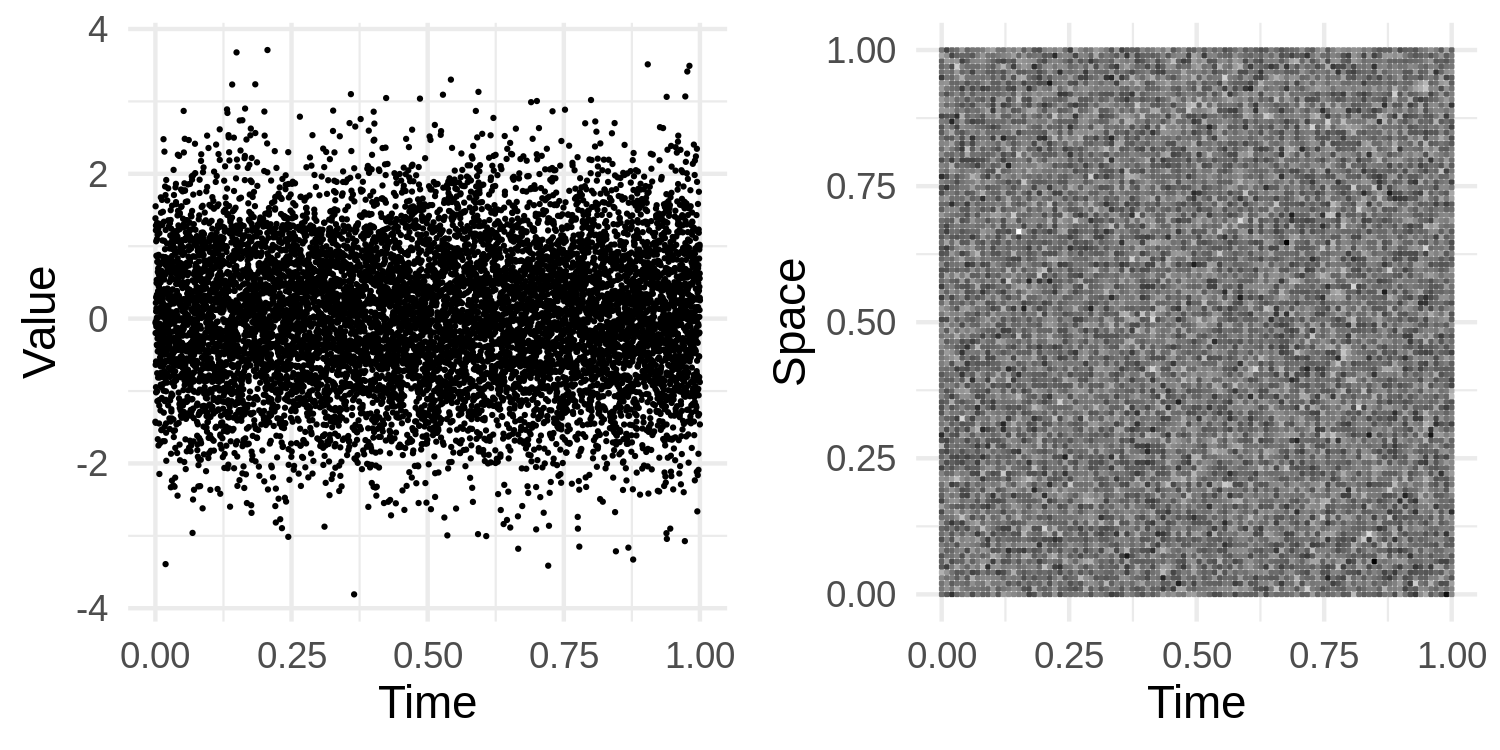
\includegraphics{wn} 

}

\caption{\label{wn}Approximations of sample paths of temporal white noise (left) and space-time white noise (right) with brightness scaled to value.}\label{fig:unnamed-chunk-2}
\end{figure}

However, it turns out that realizations of white noise do not exist as
functions in the classical sense. Indeed, since Brownian motion is
nowhere differentiable with respect to time, white noise cannot be
formally understood as a time derivative. Thus our notation \(\dot W\)
is only meant to aid intuition and not be taken as formal. A formal
understanding is possible by considering white noise as a
\emph{measure}-valued process (Dawson 1975; Walsh 1986) or as a
\emph{generalized} process that acts on classically defined functions or
stochastic processes to return either random variables or stochastic
processes (Krylov and Rozovskii 1981; Da Prato and Zabczyk 2014). Since
a measure-valued process can be defined from a generalized process and a
generalized process can be defined from a measure-valued process, the
distinction between the two is more or less a matter of perspective.
However, we find the perspective of white-noise as a generalized process
to be a more efficient route for developing heuristics to help with some
routine calculations involved with deriving SDE from SPDE. Hence, the
notion of a generalized process provides the general idea implemented
here. Although the treatments of SPDE provided by Krylov and Rozovskii
(1981) and Da Prato and Zabczyk (2014) extend the theory of SDE to
formally treat SPDE in a general and elegant fashion, they require the
navigation of an enourmous amount of technical definitions and detailed
proofs. To extract some particularly useful results from this theory
relevant to our goal of synthesizing the stochastic dynamics of
biological populations, we provide a streamlined approach by
capitolizing on the solid ground these authors have established. For
instance, instead of rigorously proving properties of white-noise, we
simply define them to be so, taking solice in the fact that the
technical details have been worked out elsewhere. In SM \S\ref{DPZ14} we
show how our informal treatment is related to the rigorous treatment
provided by Da Prato and Zabczyk (2014).

Before diving in, we shed a bit of light on the idea of a generalized
process. A generalized process is the stochastic analog of a generalized
function, such as the Dirac delta function \(\delta\). Often one sees
\(\delta\) defined as a function satisfying the properties
\(\delta(x)=0\) for \(x\neq0\) and
\(\int_{-\infty}^{+\infty}\delta(x)dx=1\). However, since there is no
function that satisfies these properties, we refer to \(\delta\) as a
generalized function. An alternative definition of \(\delta\) considers
its action on classically defined functions \(f\). In particular,
\(\delta(f)=f(0)\), which can be heuristically written as
\(\int_{-\infty}^{+\infty}f(x)\delta(x)dx=f(0)\). Similarly, other
generalized functions can be defined by their action on classically
defined functions. Then, just as a generalized function operates on
classical functions to return a value, a generalized process acts on a
set of functions (or processes) to return a random variable (or a
classically defined stochastic process). For a brief primer on the
theory of generalized functions, see the addendum to chapter 3 of
Kolmogorov and Fomin (1999).

\hypertarget{definition-and-basic-properties-of-white-noise}{%
\subsubsection{\texorpdfstring{Definition and basic properties of white
noise
\label{wnc_intro}}{Definition and basic properties of white noise }}\label{definition-and-basic-properties-of-white-noise}}

Throughout this section, we minimize notation by writing
\(\int_{\mathbb{R}}f(x)dx=\int_{-\infty}^{+\infty}f(x)dx\) and similarly
\(\int_Df(x)dx\) for the integral of \(f\) over \(D\subset\mathbb{R}\).
We define \(\mathscr{N}_2\) as the set of stochastic processes
\(f(x,t)\) that are continuous in \(t\) and satisfy
\(\mathbb{E}\left(\int_0^t\int_\mathbb{R}f^2(x,s)dxds\right)<+\infty\)
for each \(t\geq0\). The operator \(\mathbb{E}\) denotes expectation
with respect to the underlying probability space. For each \(t\geq0\) we
set

\begin{equation}
\|f\|_t=\sqrt{\mathbb{E}\left(\int_0^t\int_\mathbb{R}f^2(x,s)dxds\right)},
\end{equation}

and make use of the convention \(f=g\) if \(\|f-g\|_t=0\) for all
\(t\geq0\). Later, when we investigate stochastic dynamics of the
abundance density \(\nu(x,t)\), we will find
\(\sqrt\nu\in\mathscr{N}_2\). This enables us to utilize the heuristics
developed in this section for the derivation of SDE describing the
stochastic dynamics of \(N(t)\), \(\bar x(t)\) and \(\sigma^2(t)\).

We define a generalized stochastic process \(\mathbf W\) that maps
processes \(f\in\mathscr{N}_2\) to real-valued stochastic processes
indexed by time \(t\geq0\), but not by space. To evaluate \(\mathbf W\)
for a process \(f\in\mathscr{N}_2\) and some time \(t\geq0\) we write
\(\mathbf W_t(f)\). Specifically, for any \(f,g\in\mathscr{N}_2\), we
define \(\mathbf W(f)\) and \(\mathbf W(g)\) to be Gaussian processes
satisfying, for any \(t,t_1,t_2\geq0\), \begin{equation}\label{exp_WN}
\mathbb{E}\big(\mathbf W_t(f)\big)=\mathbb{E}\big(\mathbf W_t(g)\big)=0,
\end{equation} \begin{equation}\label{cov_WN}
\mathbb{C}\big(\mathbf W_{t_1}(f),\mathbf W_{t_2}(g)\big)=\mathbb{E}\left(\int_0^{t_1\wedge t_2}\int_\mathbb{R} f(x,s)g(x,s)dxds\right),
\end{equation} where \(t_1\wedge t_2=\min(t_1,t_2)\) and \(\mathbb{C}\)
denotes covariance with respect to the underlying probability space. In
particular, denoting \(\mathbb{V}\) the variance operator with respect
to the underlying probability space, we have
\(\mathbb{V}\big(\mathbf W_t(f)\big)=\|f\|_t^2\) for all \(t\geq0\) and
\(f\in\mathscr{N}_2\). The operators \(\mathbb{E}\) and \(\mathbb{C}\)
are to be distinguished from \(\bar f(t)\) and \(\mathrm{Cov}_t(f,g)\)
which denote expectation and covariance with respect to phenotypic
diversity at time \(t\geq0\).

Since Gaussian processes are characterized by their expectations and
covariances and since we assume the \(\mathscr{N}_2\) processes are
continuous in time, the processes \(\mathbf W(f)\) and \(\mathbf W(g)\)
are well defined. As an example, if \(f\in\mathscr{N}_2\) is independent
of time, then \(\mathbf W(f)\) is a Brownian motion with variance at
time \(t\geq0\) equal to
\(\|f\|_t^2=t \ \mathbb{E}(\int_\mathbb{R}f^2(x,0)dx)\). With the
generalized process \(\mathbf W\) defined, we define the space-time
white noise \(\dot W(x,t)\) implicitly via the stochastic integral
\begin{equation}\label{informal}
``\int_0^t\int_\mathbb{R}f(x,s)\dot W(x,s)dxds"=\mathbf W_t(f), \ \forall \ f\in\mathscr{N}_2, \ t\geq0.
\end{equation} We place quotations in the above expression to emphasize
its informal nature and that it should not be confused with classical
Riemann integration. Following this definition of white noise, we
compute its value by sampling it using \(\mathscr{N}_2\) processes. For
example, integrating white noise over a region \(D\times[0,t]\), with
\(t>0\) and \(D\) a bounded subset of \(\mathbb{R}\), is equivalent to
evaluating \(\mathbf W_t(I_{D\times [0,+\infty)})\) for the
deterministic process \begin{equation}
I_{D\times [0,+\infty)}(x,t)=\left\{\begin{matrix}
0, & x\notin D \\
1, & x\in D
\end{matrix}\right..
\end{equation} Since \begin{equation}
\|I_{D\times[0,+\infty))}\|_t^2=\mathbb{E}\left(\int_0^t\int_\mathbb{R}I_{D\times [0,+\infty)}^2(x,s)dxds\right)=t\int_Ddx=t|D|<+\infty, 
\end{equation} where \(|D|\) denotes the length of \(D\), we have
\(I_{D\times [0,+\infty)}\in\mathscr{N}_2\). Thus, using equations
(\ref{exp_WN}) and (\ref{cov_WN}) and adopting the informal notation
introduced in equation (\ref{informal}), we can write the following
\begin{equation}
\mathbb{E}\left(\int_0^t\int_D\dot W(x,s)dxds\right)=0,
\end{equation} \begin{equation}
\mathbb{V}\left(\int_0^t\int_D\dot W(x,s)dxds\right)=t|D|.
\end{equation} Using this informal notation, equations (\ref{exp_WN})
and (\ref{cov_WN}) can be rewritten as \begin{equation}\label{exp_WN_xi}
\mathbb{E}\left(\int_0^t\int_\mathbb{R}f(x,s)\dot W(x,s)dxds\right)=0,
\end{equation} \begin{equation}\label{cov_WN_xi}
\mathbb{C}\left(\int_0^{t_1}\int_\mathbb{R}f(x,s)\dot W(x,s)dxds,\int_0^{t_2}\int_\mathbb{R}g(x,s)\dot W(x,s)dxds\right)
=\int_0^{t_1\wedge t_2}\int_\mathbb{R}f(x,s)g(x,s)dxds.
\end{equation} To relate these formulae to the common notation used for
SDE, we write \begin{equation}
\hat f(x,t)=\frac{f(x,t)}{\sqrt{\int_\mathbb{R}f^2(y,t)dy}} \ \text{ and } \ 
d\hat{\mathbf W}_t(f)=\left(\int_\mathbb{R}\hat f(x,t)\dot W(x,t)dx\right)dt
\end{equation} so that \begin{equation}
\int_0^td\hat{\mathbf W}_s(f)=\int_0^t\int_\mathbb{R}\frac{f(x,s)}{\sqrt{\int_\mathbb{R}f^2(s,y)dy}}\dot W(x,s)dxds.
\end{equation} This implies \begin{equation}
\mathbb{E}\left(\int_0^td\hat{\mathbf W}_s(f)\right)=0, \ \mathbb{C}\left(\int_0^{t_1}d\hat{\mathbf W}_s(f),\int_0^{t_2}d\hat{\mathbf W}_s(f)\right)=t_1\wedge t_2
\end{equation} and in particular, as a function of \(t\),
\(\int_0^td\hat{\mathbf W}_s(f)\) is a standard Brownian motion for any
\(f\in\mathscr{N}_2\). Hence, \(d\hat{\mathbf W}_t(f)\) is analogous to
the traditional shorthand used to denote stochastic differentials. Thus,
equation (\ref{cov_WN_xi}) effectively extends Itô's multiplication
table to:

\begin{table}[H]
\centering\caption{An extension of It\^o's multiplication table.}\vspace{0.2cm}
\begin{tabular}{l|lll}
             & $d\hat{\mathbf W}_t(f)$               & $d\hat{\mathbf W}_t(g)$                & $dt$ \\ \hline
             &                            &                            &      \\
$d\hat{\mathbf W}_t(f)$ & $dt$                       & $\left(\int_\mathbb{R}\hat f(x,t)\hat g(x,t)dx\right)dt$ & $0$  \\
             &                            &                            &      \\
$d\hat{\mathbf W}_t(g)$ & $\left(\int_\mathbb{R}\hat f(x,t)\hat g(x,t)dx\right)dt$ & $dt$                       & $0$  \\
             &                            &                            &      \\
$dt$         & $0$                        & $0$                        & $0$
\end{tabular}\label{mult}
\end{table}

The extension of Itô's multiplication table and properties of white
noise outlined in this subsection provide a useful set of tools for
working with SPDE. In SM \S\ref{SDE_DERIV} we employ these tools to
derive SDE that track the dynamics of abundance, mean trait and
phenotypic variance of a population from a particular SPDE. In the
following subsection, we review how this particular SPDE naturally
arises as the diffusion limit of a BBM.

\hypertarget{from-branching-processes-to-spde}{%
\subsubsection{\texorpdfstring{From branching processes to SPDE
\label{stochastic}}{From branching processes to SPDE }}\label{from-branching-processes-to-spde}}

In real populations individuals are born and potentially reproduce
before they ultimately die. These three events provide the basic
ingredients of a branching process. Mathematical investigations of such
processes have a relatively deep history (Kendall 1966). The most simple
branching process, known as the Galton-Watson process, describes the
number of individuals alive at a given time \(t\geq0\) as a non-negative
integer (Kimmel and Axelrod 2015). Feller (1951) introduced a formal
method to approximate branching processes with diffusion processes which
are continuous in state (i.e., population size is approximated as a
continuous quantity). Since diffusion processes possess greater
analytical tractability than branching processes, Feller's method, known
as the diffusion limit, has acquired immense popularity particularly in
the field of mathematical population genetics (Ewens 2004). For over the
past half of a century a great deal of accomplishments have been
achieved in formalizing the diffusion limits of branching processes that
describe populations of individuals occuring in some continuous space
(Watanabe 1968; Dawson 1975, 1978; Perkins 1992, 1995; Méléard and
Roelly 1993; Li 1998; Bertoin and Le Gall 2003; Etheridge 2008; Barton
and Etheridge 2019). This space can represent geographic space or,
relevant to our context, phenotypic space. In the following subsection,
we describe the BBM process, which is a particularly important branching
process with spatial stucture. This process has been very useful in the
study of SPDE due to its simplifying assumption that individuals do not
interact. However, this assumption imposes an unfortunate restriction by
precluding the modelling of ecological interactions. We therefore follow
our discussion of BBM with a review of a few important results on
spatially structured branching processes that account for interactions.

\textbf{Branching Brownian motion}

A BBM tracks individuals navigating \(d\)-dimensional Euclidean space
that reproduce and senesce between exponentially distributed intervals.
Unlike other stochastic processes that take values in \(\mathbb{R}^d\),
BBM takes values in the set of \emph{non-negative finite measures} over
\(\mathbb{R}^d\). Intuitively, one can think of a finite measure as a
function that maps subsets of \(\mathbb{R}^d\) to real numbers. To be
formal, we only consider the Borel subsets of \(\mathbb{R}^d\)
corresponding to the Euclidean metric, but understanding this
technicality is not crucial to our discussion. In particular, denoting
\(X_t\) a BBM, for a subset \(D\subset\mathbb{R}^d\), \(X_t(D)\) returns
the (random) number of individuals alive within the region \(D\) at time
\(t\geq0\). The BBM has three main components:

\begin{enumerate}
\def\labelenumi{\arabic{enumi})}
\item
  \textbf{Branching rate:} In our formulation of BBM we assume Lifetimes
  of individuals are exponentially distributed with death rate
  \(\lambda>0\) and reproduction occurs simultaneously with death.
  Biologically, this implies individuals are semelparous An alternative
  formulation treats birth and death events separately to model
  iteroparity. However, under the appropriate rescaling, both approaches
  converge to the same diffusion limit. We therefore choose the former
  approach for the sake of simplicity.
\item
  \textbf{Reproductive law:} When a birth event occurs a random
  (possibly zero) number of offspring are left. The distribution of
  offspring left is called the reproductive law or branching mechanism.
  We denote the mean and variance in reproductive output by
  \(\mathscr{W}\) and \(V\) respectively. The case of \(\mathscr{W}=1\)
  is referred to as the critical condition. Under the critical condition
  the probability that extinction occurs in finite time is equal to one.
\item
  \textbf{Spatial movement:} Each offspring is born at the current
  location of their parent. Immediately after birth they move around
  space according to \(d\)-dimensional Brownian motion with diffusion
  parameter \(\sqrt\mu\). In our context we interpret spatial movement
  as mutation so that the location of an individual at death represents
  the value of its phenotype. Then an individual born at location
  \(x\in\mathbb{R}^d\) that lives for \(\tau>0\) units of time will have
  a normally distributed trait centered on \(x\) with covariance matrix
  equal to \(\tau\mu\) times the \(d\times d\) identity matrix. Hence,
  offspring inherit normally distributed traits centered on their
  parental trait. This fact creates a vital link to the deterministic
  dynamics reviewed above. Indeed, in the absence of selection, the
  deterministic PDE (\ref{eq1}) reduces to the \(d=1\)-dimensional
  Kolmogorov forward equation for a Brownian motion with diffusion
  parameter \(\sqrt\mu\).
\end{enumerate}

To obtain a SPDE from a BBM we take a diffusion limit. There are several
ways to do this, but a simple approach is to rescale the mass of
individuals and time by \(1/n\), diffusion by \(\mu\to\mu/n\), branching
rate by \(\lambda\to n\lambda\), fitness by
\(\mathscr{W}\to\mathscr{W}^{1/n}\) and consider the limit as
\(n\to\infty\). Denoting the rescaled process by \(X_t^{(n)}(D)\), the
limiting process \(\mathscr{X}_t=\lim_{n\to\infty}X_t^{(n)}\) is called
a super-Brownian motion and is also a non-negative finite measure-valued
process (Watanabe 1968). However, instead of returning the number of
individuals alive in a region of space, super-Brownian motion returns
the \emph{mass} of the population concentrated in a region of space.
Since we have rescaled individual mass by \(1/n\) and took the limit
\(n\to\infty\), individuals are no longer discrete units. Instead, the
particle view of the population gets replaced by a blob spread across
\(d\)-dimensional space. In particular, the value of
\(\mathscr{X}_t(D)\) is a continuously varying non-negative random
variable for any \(t\geq0\) and \(D\subset\mathbb{R}^d\).

Unfortunately, just as with cream cheese spread across too much toast,
the blob perspective of the population may exhibit some complicated
spatial discontinuities. However, for spatial dimension \(d=1\), it
turns out that \(\mathscr{X}_t\) is absolutely continuous with respect
to the Lebesgue measure for each \(t\geq0\) (Konno and Shiga 1988;
Reimers 1989). This means that we can write
\(\mathscr{X}_t(D)=\int_D \nu(x,t)dx\) for some density process
\(\nu(x,t)\). Setting \(\lambda=1\) and \(m=\ln\mathscr{W}\) this
density process satisfies the SPDE \begin{equation}\label{neutral_SPDE}
\frac{\partial}{\partial t}\nu(x,t)=m\nu(x,t)+\frac{\mu}{2}\frac{\partial^2}{\partial x^2}\nu(x,t)+\sqrt{V\nu(x,t)}\dot W(x,t).
\end{equation} Since \(\nu(x,t)\) is not generally differentiable in
\(x\) or \(t\), the derivatives in expression (\ref{neutral_SPDE}) are
taken in the \emph{weak} sense (for examples, see Evans 2010). That is,
to rigorously interpret SPDE (\ref{neutral_SPDE}), we integrate the
solution \(\nu(x,t)\) against functions \(f\in C_b^2(\mathbb{R})\),
where \(C_b^2(\mathbb{R})\) is the set of bounded and twice continuously
differentiable functions on \(\mathbb{R}\). Hence, equation
(\ref{neutral_SPDE}) is just an abbreviation for

\begin{multline}\label{neutral_int}
\int_\mathbb{R}\nu(x,t)f(x)dx-\int_\mathbb{R}\nu(x,0)f(x)dx=\int_0^t\int_\mathbb{R}\nu(x,s)\left(mf(x)+\frac{\mu}{2}\frac{\partial^2}{\partial x^2}f(x)\right)dsdx \\
+\int_0^t\int_\mathbb{R}f(x)\sqrt{V\nu(x,s)}\dot W(x,s)dxds, \ \forall \ f\in C_b^2(\mathbb{R}).
\end{multline} This expression is referred to as the \emph{mild}
solution of (\ref{neutral_SPDE}). For more on the general theory of SPDE
see Walsh (1986) and Da Prato and Zabczyk (2014). Note that since
\(\nu(x,t)\) is the density of a finite measure, it is integrable for
each \(t\geq0\). Thus, since for some \(M>0\), \(|f(x)|\leq M\) for
every \(x\in\mathbb{R}\), setting \(\varphi(x,t)=f(x)\sqrt{V\nu(x,t)}\)
implies \(\varphi\in\mathscr{N}_2\). Hence, the white noise integral on
the right-hand side of equation (\ref{neutral_int}) can be understood
using the heuristics introduced above. Evaluating equation
(\ref{neutral_int}) in the particular case of \(f(x)\equiv1\) returns
the total mass process, which we refer to as the total abundance
\(N(t)\).

A convergence theorem for the diffusion limit of a generalization of BBM
was established by Watanabe (1968). Dawson (1975) suggested that, for
spatial dimension \(d=1\), this diffusion limit should admit a density
process that satisfies a SPDE. Konna and Shiga (1988) and Reimers (1989)
independently proved Dawson's suggestion was indeed correct. The
diffusion limit of this more general branching process (in arbitrary
spatial dimension) is referred to as a Dawson-Watanabe superprocess
(Etheridge 2000). Conditioning a Dawson-Watanabe superprocess to have
constant mass returns a Fleming-Viot process (Etheridge and March 1991;
Perkins 1991) which has been popular in studies of spatial population
genetics. In particular, an extension of the Fleming-Viot process, known
as the \(\Lambda\)-Fleming-Viot process, was introduced by Bertoin and
Le Gall (2003) and coined by Etheridge (2008) where it was used to
resolve some technical challenges in modelling isolation by distance
(Felsenstein 1975; see also Barton, Etheridge, and Véber 2013; and
Barton and Etheridge 2019). Although this provides an impressive list of
accomplishments, the Dawson-Watanabe superprocess falls short of our
needs. In particular this process assumes individuals do not interact
and thus precludes its ability to model nonlocal effects on the fitness
of individuals, such as those produced via ecological interactions.
However, this concern has been addressed, leading to constuctions of
superprocesses that account for interactions among individuals. In the
next subsection we summarize the main results in this area and introduce
the SPDE that provides the basis for our approach to theoretical
evolutionary ecology.

\textbf{Interacting superprocesses}

In the above subsection we reviewed the diffusion limit of an especially
tractable measure-valued branching process. However, we found the
simplicity of this process restricts us from modelling nonlocal effects
on the fitness of individuals. Here, we discuss superprocesses that
account for such effects. The existence of diffusion limits for a class
of measure-valued branching processes involving nonlocal effects has
been treated by Méléard and Roelly (1992, 1993). The interactions can
manifest as dependencies of the spatial movement or reproductive law of
individuals on their position \(x\) and the state of the whole
population described by \(X_t\). An important result of Méléard and
Roelly (1992, 1993) is a theorem that provides sufficient conditions to
construct a sequence of rescaled measure-valued branching processes that
converge to a generalization of the Dawson-Watanabe superprocess that
includes interactions. The rescaling is analogous to that described
above for non-interacting Dawson-Watanabe superprocesses, but now the
reproductive law described by \(\mathscr{W}(X_t,x)\) and \(V(X_t,x)\),
branching rate \(\lambda(X_t,x)\) and diffusion parameter
\(\sqrt{\mu(X_t,x)}\) are allowed to depend on the whole population
\(X_t\) and individual location \(x\). In Figure \ref{rescaled} we
demonstrate this rescaling in discrete time for a population
experiencing stabilizing selection and logistic growth. Since time is
discretized, the process we simulate is formally a branching random
walk. For further details on our simulation see SM \S\ref{numerical}.

\begin{figure}

{\centering 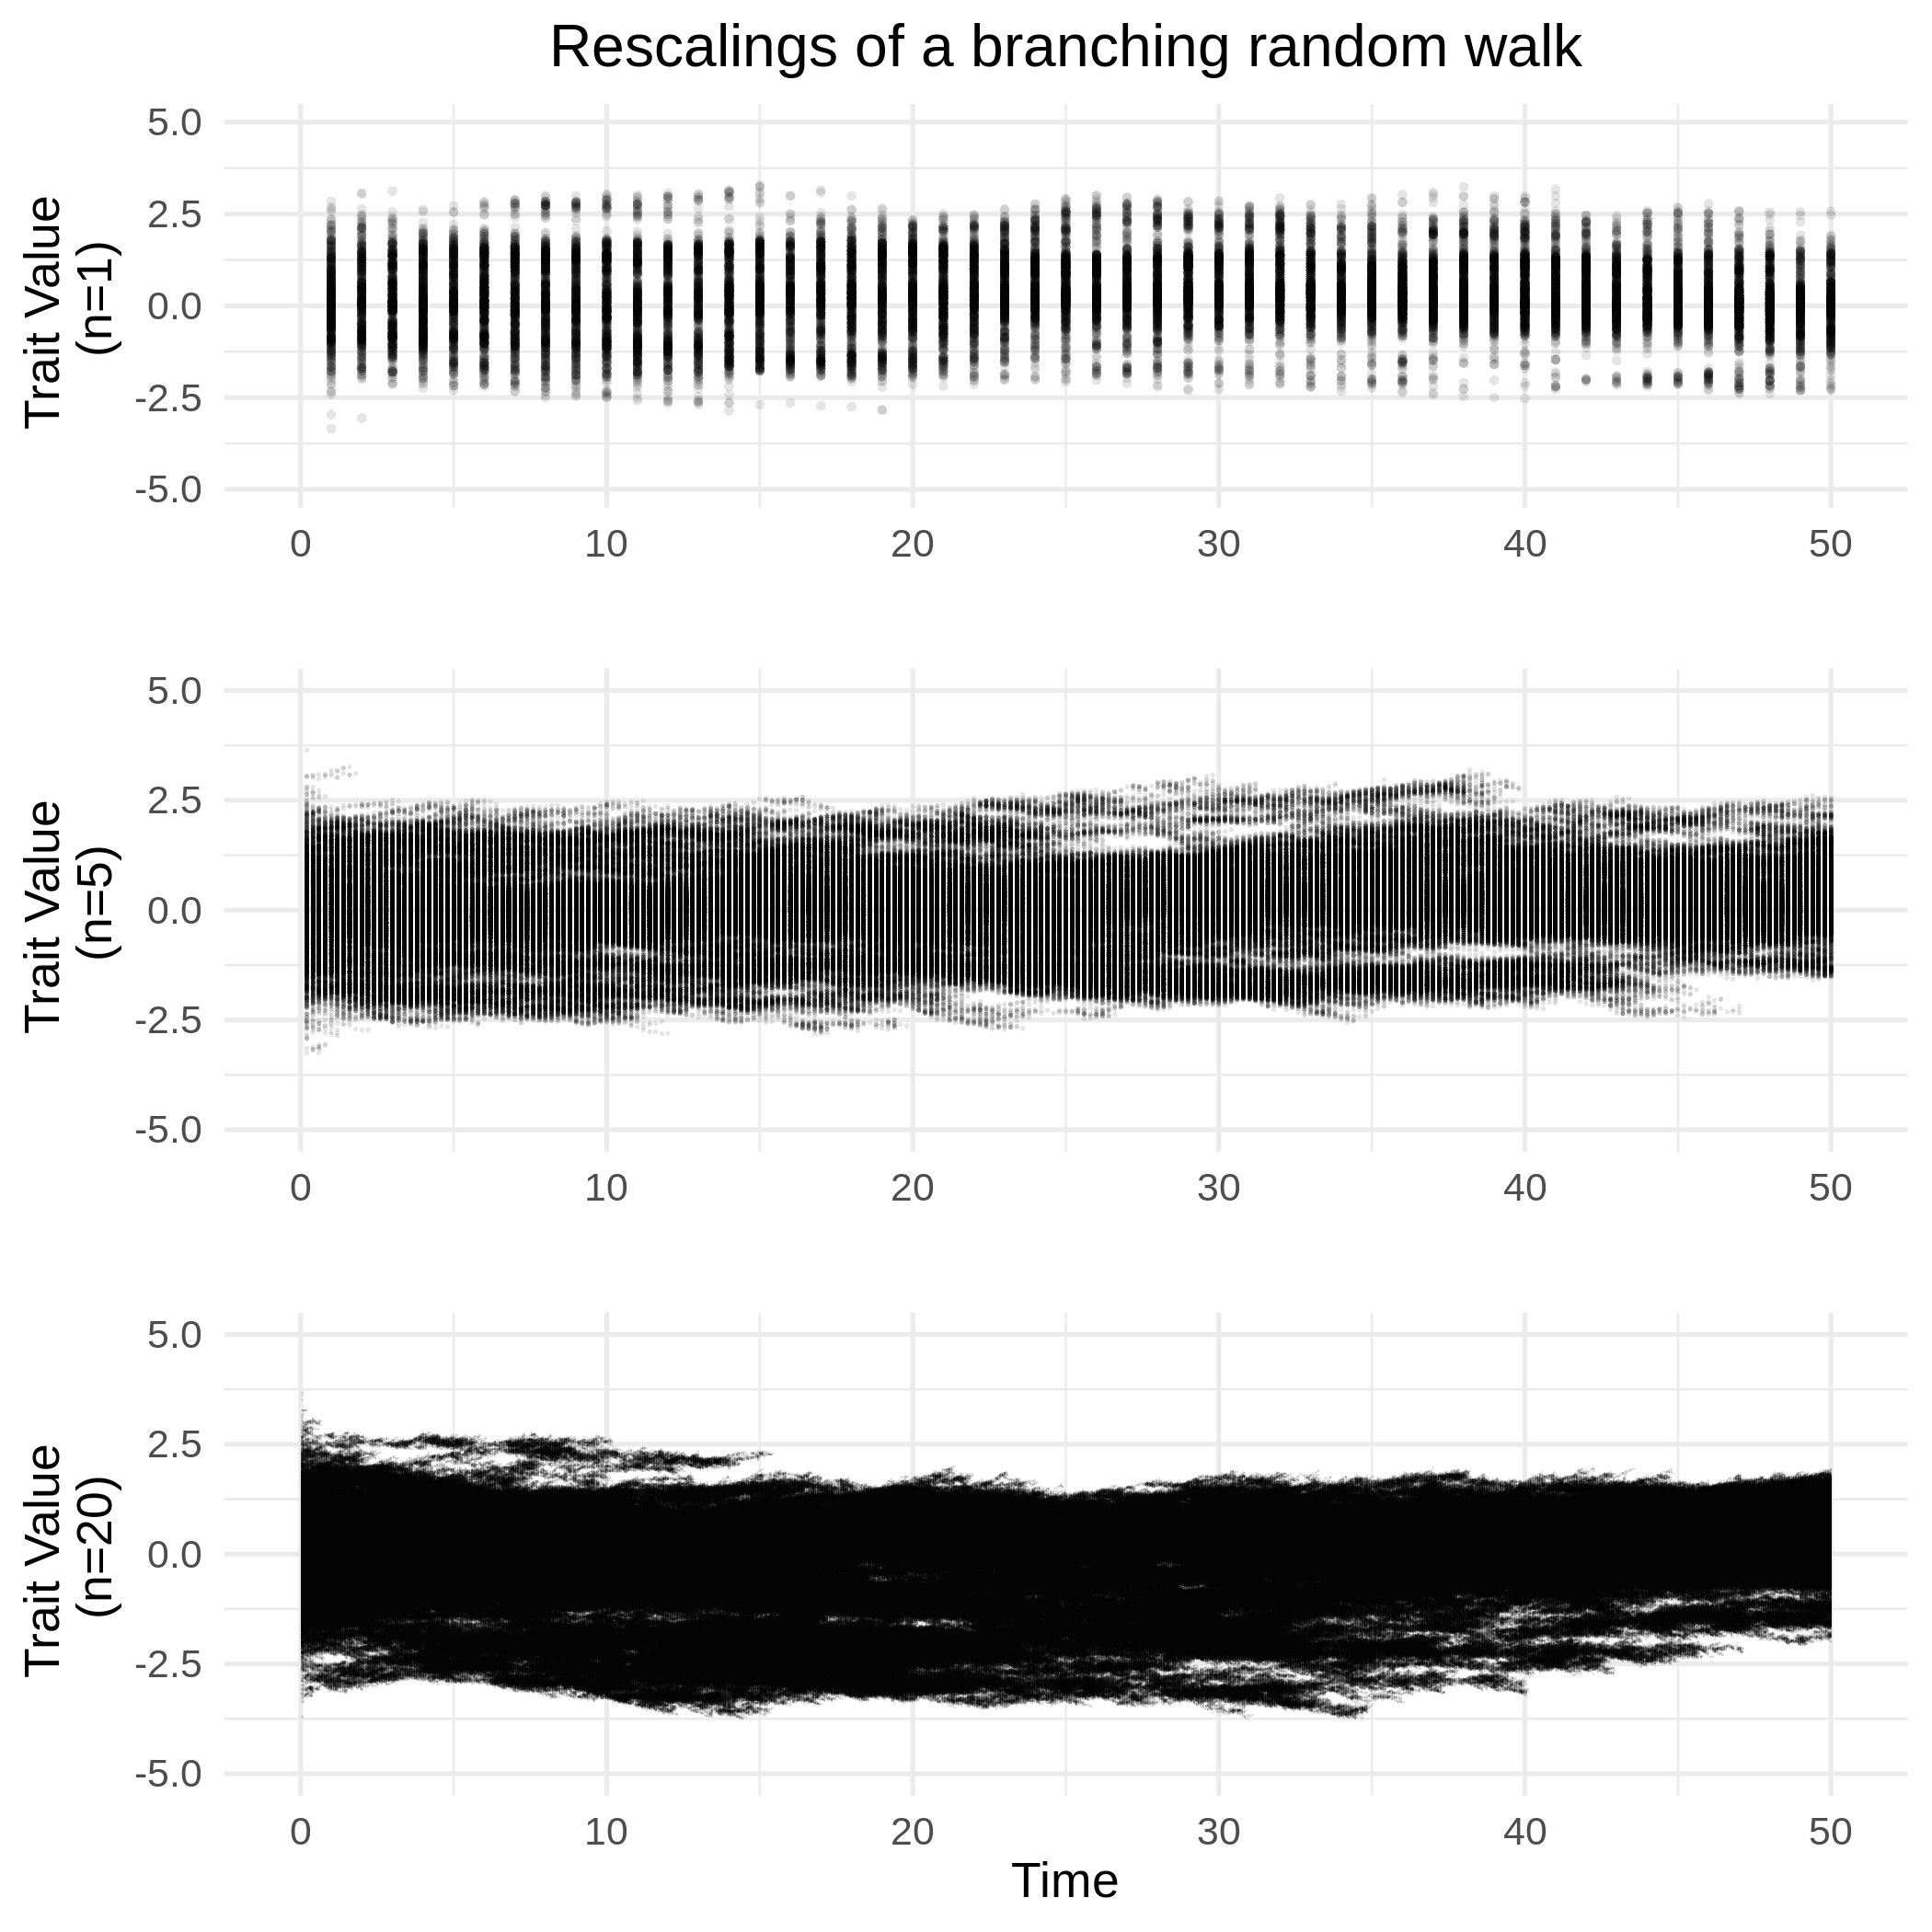
\includegraphics{rescaled_plots} 

}

\caption{\label{rescaled}Rescaled sample paths of a branching random walk under stabilizing selection and logistic growth. The top plot displays a sample path without scaling $(n=1)$, the middle plot shows a sample path rescaled by $n=5$ and the bottom plot shows a sample path rescaled by $n=20$.}\label{fig:unnamed-chunk-4}
\end{figure}

Interactions that manifest in the spatial movement can be used to model
mutation bias and those manisfesting in the reproductive law can model
density-dependent growth rates and frequency-dependent selection.
Perkins (1992, 1995) developed a theory of stochastic integration with
respect to the so-called \emph{Brownian trees} to characterize
interacting superprocesses and establish properties of existence and
uniqueness. Li (1998) built directly off of the construction of Méléard
and Roelly (1992, 1993) to study properties of density processes
associated with interacting superprocesses, arriving at a SPDE that
forms the foundation of our approach.

Recall, we use \(\nu(x,t)\) to denote the density of a superprocess,
given it exists. Assuming the interactions manifest only in the
reproductive law and that spatial movement follows Brownian motion with
diffusion parameter \(\sqrt\mu\) independent of both \(X_t\) and \(x\),
Li (1998) proved a result that implies the interacting superprocess on
one dimensional trait space has a density \(\nu(x,t)\) which is
non-negative, integrable, continuous in time and space and satisfies the
SPDE \begin{equation}\label{SPDE}
\frac{\partial}{\partial t}\nu(x,t)=m(\nu,x)\nu(x,t)+\frac{\mu}{2}\frac{\partial^2}{\partial x^2}\nu(x,t)+\sqrt{V\nu(x,t)}\dot W(x,t).
\end{equation} As mentioned above, we refer to SPDE (\ref{SPDE}) as the
Stochastic Asexual Gaussian allelic model with Abundance dynamics
(abbreviated SAGA). Comparing equation (\ref{SPDE}) to equation (3.5) of
Li (1998), our \(m\) and \(V\) correspond to Li's \(b\) and \(c\)
respectively. It is important to note that, under the assumptions made
in Méléard and Roelly (1992, 1993) and Li (1998), equation (\ref{SPDE})
is only formal when \(m(h,x)\) is bounded across all combinations of
\(h\geq0\) and \(x\in\mathbb{R}\). However, recalling our condition
\(m(h,x)\leq r\in\mathbb{R}\), the growth rates we consider are only
bounded above. Yet, in the proof of the construction of the interacting
superprocess as the limit of rescaled branching diffusions, Méléard and
Roelly (1992, 1993) assumed \(m(h,x)\) to be bounded to guarantee the
total mass process will have finite mean and variance, for finite
\(t\geq0\). This allowed the authors to employ a tightness criterion for
sequences of measures and show the rescaled processes converge to a
superprocess with finite total mass. Li's (1998) result builds directly
off of Méléard and Roelly's construction, inheriting the assumption of
boundedness for \(m(h,x)\). However, in Li (1998), the sufficiency of
\(m(h,x)\) being bounded above is even more clear since Li works
explicitly with a common upperbound for both \(m(h,x)\) and \(V\).
Hence, one can repeat the necessary proofs replacing the assumption that
\(m(h,x)\) is bounded with the assumption that \(m(h,x)\) is merely
bounded above to derive the same results. An alternative approach to
establishing this result that allows for our relaxed assumption on the
growth rate has carried out by Champagnat, Ferrière, and Méléard (2006)
using techniques developed by Evans and Perkins (1994).

With solutions to SPDE (\ref{SPDE}) well defined for any growth rate
bounded above, we can calculate the total mass process \(N(t)\) using
the mild solution of (\ref{SPDE}) with
\(f(x)\equiv1\in C_b^2(\mathbb{R})\) (the symbol ``\(\equiv\)'' means
equal to for every \(x\)). That is,

\begin{multline}
N(t)=N(0)+\int_0^t\int_\mathbb{R}\nu(x,s)\left(m(\nu,x)\cdot1+\frac{\mu}{2}\frac{\partial^2}{\partial x^2}1\right)+1\sqrt{V\nu(x,s)}\dot W(x,s)dsdx \\
=N(0)+\int_0^t\bar m(s)N(s)dt+\int_0^t\sqrt{VN(s)}d\hat{\mathbf{W}}_s(\sqrt{\nu(x,s)}),
\end{multline} where \begin{equation}
\bar m(t)=\frac{1}{N(t)}\int_\mathbb{R}m(\nu,x)\nu(x,t)dx,
\end{equation} and \begin{equation}
\int_0^td\hat{\mathbf{W}}_s(\sqrt{\nu(x,s)})=\int_0^t\int_\mathbb{R}\frac{\sqrt{\nu(x,s)}}{\sqrt{\int_\mathbb{R}\nu(x,s)dx}}\dot W(x,s)dxds.
\end{equation} Setting \(W_1(t)=\hat{\mathbf{W}}_t(\sqrt{\nu(x,t)})\),
we can use traditional stochastic differential notation to write
\begin{equation}
dN=\bar mNdt+\sqrt{VN}dW_1.
\end{equation} To find the associated SDE for \(\bar x(t)\) and
\(\sigma^2(t)\), we want to repeat the same approach for \(f(x)=x,x^2\)
and apply Itô's lemma. However, for these cases
\(f\notin C^2_b(\mathbb{R})\) since \(f\) will not be bounded. But if we
can show \(\int_\mathbb{R}(|x|+x^2+x^4)\nu(x,t)dx<+\infty\) for all
\(t>0\) given this condition is satisfied by \(\nu(x,0)\), then we can
apply the mild solution of (\ref{SPDE}) to derive SDE for \(\bar x(t)\)
and \(\sigma^2(t)\). To illustrate, let us suppose this is the case.
Setting \(\tilde x(t)=\int_\mathbb{R}x\nu(x,t)dx\), we have
\begin{equation}
\tilde x(t)=\tilde x(0)+\int_0^t\int_\mathbb{R}\nu(x,s)m(\nu,x)x+x\sqrt{V\nu(x,s)}\dot W(x,s)dxds.
\end{equation} Similarly, setting
\(\tilde{\tilde\sigma}^2(t)=\int_\mathbb{R}x^2\nu(x,t)dx\), we have
\begin{equation}
\tilde{\tilde\sigma}^2(t)=\tilde{\tilde\sigma}^2(0)+\int_0^t\int_\mathbb{R}\nu(x,s)\left(m(\nu,x)x^2+\mu\right)+x^2\sqrt{V\nu(x,s)}\dot W(x,s)dxds.
\end{equation} Since \(\bar x(t)=\tilde x(t)/N(t)\) and
\(\sigma^2(t)=\tilde{\tilde\sigma}^2(t)/N(t)-\bar x^2(t)\), we can use
Itô's lemma to derive SDE for \(\bar x(t)\) and \(\sigma^2(t)\), which
we perform in SM \S\ref{SDE_DERIV}. We make no attempt in finding
sufficient conditions for
\(\int_\mathbb{R}(|x|+x^2+x^4)\nu(x,t)dx<+\infty\) to hold and hence
make no general assertions about the existence or uniqueness of
\(\bar x(t)\) or \(\sigma^2(t)\). Regardless, we will later assume
\(\nu(x,t)\) can be approximated by a Gaussian curve in \(x\) for all
\(t\geq0\). This assumption implies
\(\int_\mathbb{R}|x|^n\nu(x,t)dx<+\infty\) for all \(n\in\mathbb{N}\)
and for all \(t\geq0\).

\hypertarget{equations-of-evolutionary-and-demographic-dynamics}{%
\subsection{\texorpdfstring{Equations of evolutionary and demographic
dynamics
\label{equations}}{Equations of evolutionary and demographic dynamics }}\label{equations-of-evolutionary-and-demographic-dynamics}}

In SM \S\ref{SDE_DERIV} we show SDE for \(N(t)\), \(\bar x(t)\) and
\(\sigma^2(t)\) can be expressed as

\begin{subequations}\label{gen_eqns}
\begin{equation}\label{N}
dN(t)=\bar m(t)N(t)dt+\sqrt{V N(t)}dW_1(t),
\end{equation}
\begin{equation}\label{xbar_gen}
d\bar x(t)=\mathrm{Cov}_t\Big(x,m(\nu,x)\Big)dt+\sqrt{V\frac{\sigma^2(t)}{N(t)}}dW_2(t),
\end{equation}
\begin{equation}\label{sig2_gen}
d\sigma^2(t)=\mathrm{Cov}_t\Big((x-\bar x(t))^2,m(\nu,x)\Big)dt+\left(\mu-V\frac{\sigma^2(t)}{N(t)}\right)dt+\sqrt{V\frac{\overline{(x-\bar x(t))^4}-\sigma^4(t)}{N(t)}}dW_3(t),
\end{equation}
\end{subequations}

where \(W_1\), \(W_2\) and \(W_3\) are standard Brownian motions. We
note that conditions on the growth rate \(m\) to guarantee existence and
uniqueness of solutions to (\ref{xbar_gen}) and (\ref{sig2_gen}) have
yet to be investigated. However, our results on the deterministic PDE
suggest that \(m(h,x)\) bounded above and differentiable in both
arguments is sufficient. Dividing by \(dt\) one can interpret equations
(\ref{gen_eqns}) as if they are ordinary differential equations, but
this not technically rigorous since Brownian motion is nowhere
differentiable with respect to time. In SM \S\ref{SDE_DERIV} we show
that in general \(W_1\) is independent of both \(W_2\) and \(W_3\), but
\(W_2\) and \(W_3\) covary.

There is quite a bit we can learn from expressions (\ref{gen_eqns}).
Firstly, setting \(V=0\) recovers the deterministic dynamics derived in
\S\ref{deterministic}. Alternatively, one can take \(N(t)\to\infty\) to
recover the deterministic dynamics for \(\bar x(t)\) and
\(\sigma^2(t)\). Characteristically, we note the effect of demographic
stochasticity on abundance grows with \(\sqrt{N(t)}\). Hence, dividing
by \(N\), we find the effects of demographic stochasticity on the
per-capita growth rate diminish with increased abundance. Relating the
response to demographic stochasticity derived here to the effect of
random genetic drift derived in classic quantitative genetic theory, if
we set \(\sigma^2(t)=\sigma^2\) and \(N(t)=N\) constant with respect to
time, then integrating the stochastic term in equation (\ref{xbar_gen})
over a single unit of time returns a normally distributed random
variable with mean zero and variance equal to \(V\sigma^2/N\). In
particular, assuming perfect inheritance, when reproductive variance is
unity (\(V=1\)) this random variable coincides with the effect of random
genetic drift on the change in mean trait over a single generation
derived using sampling arguments (Lande 1976). There is also an
interesting connection with classical population genetics. A fundamental
result from early population genetic theory is the expected reduction in
diversity due to the chance loss of alleles in finite populations
(Fisher 1923; Wright 1931). This expected reduction in diversity due to
random genetic drift is captured by the third term in the deterministic
component of expression (\ref{sig2_gen}), particularly
\(-V\sigma^2(t)/N(t)\). The component of SDE (\ref{sig2_gen}) describing
random fluctuations in \(\sigma^2(t)\) is more complicated and is
proportional to the root of the difference between the centralized
fourth moment of \(p(x,t)\) and \(\sigma^4(t)\).

These expressions can be used to investigate the dynamics of the mean
and variance for general \(\nu(x,t)\). However, in the next subsection
we simplify these expressions by approximating \(\nu(x,t)\) with a
Gaussian curve. By assuming \(\nu(x,t)\) is Gaussian for \(t\geq0\), we
guarantee the existence of \(\bar x(t)\) and \(\sigma^2(t)\) for all
\(t\geq0\). Furthermore, in SM \S\ref{SDE_DERIV} we show that under the
Gaussian case \(W_1,W_2\) and \(W_3\) are independent.

\hypertarget{particular-results-assuming-a-gaussian-phenotypic-distribution}{%
\subsubsection{\texorpdfstring{Particular results assuming a Gaussian
phenotypic distribution
\label{particular}}{Particular results assuming a Gaussian phenotypic distribution }}\label{particular-results-assuming-a-gaussian-phenotypic-distribution}}

By assuming \(\nu(x,t)\) can be approximated by a Gaussian curve for
each \(t\geq0\), expressions (\ref{N}), (\ref{xbar_gen}) and
(\ref{sig2_gen}) transform into efficient tools for deriving the
dynamics of populations given a fitness function \(m(\nu,x)\). Gaussian
phenotypic distributions are often obtained through Gaussian,
exponential or weak selection approximations together with a simplified
model of inheritance and random mating (Lande 1980; Turelli 1984, 1986,
2017; Bürger 2000). Alternatively, it has been shown that a Gaussian
distribution can provide a reasonable approximation even when selection
is strong and non-Gaussian (Turelli and Barton 1994). However, our
approach adds an additional layer of difficulty. Even with Gaussian
selection, the resulting solution to SPDE (\ref{SPDE}) will only be a
Gaussian curve in expectation, assuming a Gaussian curve as the initial
condition. Yet this difficulty is not as challenging as it may first
appear. Indeed, since SPDE (\ref{SPDE}) can be derived as a diffusion
limit we know that, under the appropriate assumptions on selection,
genetic architecture and reproduction, the stochastic departure from a
Gaussian curve is negligible when the ratio \(V/N\) is small (i.e., when
the variance in reproductive output is much smaller than the population
size). In SM \S\ref{numerical} we demonstrate this result using
numerical methods. Mathematically, this requirement restricts model
parameters to regions that maintain large population sizes.
Biologically, this implies populations are not at risk of extinction.
Hence, models developed in this framework are not suitable for studying
colonization-extinction dynamics or evolutionary rescue. Allowing for
these restrictions, we may safely assume that \(\nu\) is approximately
Gaussian and justify writing \begin{equation}
\nu(x,t)=\frac{N(t)}{\sqrt{2\pi\sigma^2(t)}}\exp\left(-\frac{\big(x-\bar x(t)\big)^2}{2\sigma^2(t)}\right).
\end{equation} Under this assumption we find in SM \S\ref{cov2deriv} the
results (suppressing the dependency on \(t\))
\begin{equation}\label{covxm}
\mathrm{Cov}(x,m)=\sigma^2\left(\frac{\partial\bar m}{\partial\bar x}-\overline{\frac{\partial m}{\partial\bar x}}\right),
\end{equation} \begin{equation}
\mathrm{Cov}\Big((x-\bar x)^2,m\Big)=2\sigma^4\left(\frac{\partial\bar m}{\partial\sigma^2}-\overline{\frac{\partial m}{\partial\sigma^2}}\right)
\end{equation} and \(\overline{(x-\bar x)^4}=3\sigma^4\). Equation
(\ref{covxm}) is the continuous time equivalent to equation (9) in Lande
(1976). In particular, these results imply

\begin{subequations}\label{no_inher}
\begin{equation}\label{xbar}
d\bar x=\sigma^2\left(\frac{\partial\bar m}{\partial\bar x}-\overline{\frac{\partial m}{\partial\bar x}}\right)dt+\sqrt{V\frac{\sigma^2}{N}}dW_2,
\end{equation}
\begin{equation}\label{G}
d\sigma^2=2\sigma^4\left(\frac{\partial\bar m}{\partial\sigma^2}-\overline{\frac{\partial m}{\partial\sigma^2}}\right)dt +\left(\mu-V\frac{\sigma^2}{N}\right)dt+\sigma^2\sqrt{\frac{2V}{N}}dW_3.
\end{equation}
\end{subequations}

These equations allow us to derive the response in trait mean and
variance by taking derivatives of fitness, a much more straightforward
operation than calculating a covariance for general phenotypic
distributions. Note that in the above expressions, the partial
derivatives of \(\bar m\) represent frequency independent selection and
the averaged partial derivatives of \(m\) represent frequency dependent
selection. This relationship has already been pointed out by Lande
(1976) for the evolution of the mean trait, but here we see an analogous
relationship holds also for the evolution of trait variance.

In the next subsection we generalize this result to the case when traits
are imperfectly inherited. In this case, the phenotypic variance
\(\sigma^2\) is replaced by a genetic variance \(G\). This genetic
variance represents the component of the variance in expressed traits
\(\sigma^2\) explained by additive effects of different alleles among
genetic loci encoding for the focal phenotype (Roughgarden 1979; Bulmer
1980; Lynch and Walsh 1998). It is therefore fitting that \(G\) is
referred to as the additive genetic variance.

\hypertarget{the-evolution-of-additive-genetic-variance}{%
\subsubsection{\texorpdfstring{The evolution of additive genetic
variance
\label{inheritance}}{The evolution of additive genetic variance }}\label{the-evolution-of-additive-genetic-variance}}

To model imperfect heritability we consider the relationship between
expressed phenotypes \(x\in\mathbb{R}\) and associated genetic values
\(g\in\mathbb{R}\) known as \emph{breeding values}. The breeding value
of an individual is the sum of additive effects of the alleles carried
by the individual on its expressed trait. Since our derivations of
evolutionary equations are based on branching processes that assume
asexually reproducing populations (\S\ref{stochastic}), the additive
genetic variance \(G\) is just the variance of breeding values in a
population. For a detailed treatment of breeding values and additive
genetic variances, see Bulmer (1980) and Lynch and Walsh (1998).

Our treatment of the relationship between breeding values and expressed
traits follows classical quantitative genetic assumptions such as those
used in the seminal paper by Lande (1975) to investigate the maintenance
of genetic variation. In particular, we assume that the expressed trait
for any given individual is independent of environmental conditions and
normally distributed around their breeding value with variance \(\eta\).
Hence, \(\sigma^2=G+\eta\). In the case that all of the effects of
alleles on an expressed trait are additive, \(\eta\) is known as the
\emph{variance of environmental deviation} (Lande 1975; Lynch and Walsh
1998). For a given breeding value, we denote the probability density of
a randomly drawn expressed trait by \(\psi(x,g)\). Hence,
\begin{equation}
\psi(x,g)=\frac{1}{\sqrt{2\pi\eta}}\exp\left(-\frac{(x-g)^2}{2\eta}\right).
\end{equation} To include this relationship in our framework, we write
\(\rho(g,t)\) as the abundance density of breeding values at time \(t\)
so that
\(\int_{-\infty}^{+\infty}\rho(g,t)dg=\int_{-\infty}^{+\infty}\nu(x,t)dx=N(t)\).
We switch our focus from directly modelling the evolution of
\(\nu(x,t)\) to modelling the evolution of \(\rho(g,t)\). Once
\(\rho(g,t)\) is determined, we can compute \(\nu(x,t)\) via
\begin{equation}\label{nu_from_rho}
\nu(x,t)=\int_{-\infty}^{+\infty}\rho(g,t)\psi(x,g)dg.
\end{equation} However, since selection acts on expressed phenotypes, we
use the assumed relationship between breeding values and expressed
traits to calculate the fitness of breeding values. To motivate the
approach taken, consider the problem of inferring the breeding value of
an individual given its expressed trait \(x\). Denote \(\mathfrak{g}\) a
random variable representing the unkown breeding value. Under this model
of inheritance we know \(x\) is a random sample from a normal
distribution with mean \(\mathfrak{g}\) and variance \(\eta\).
Maximizing likelihood suggests \(x\) is our best guess for
\(\mathfrak{g}\), but the actual value of \(\mathfrak{g}\) is normally
distributed around \(x\) with the variance \(\eta\). Hence, for fixed
\(x\), we obtain \(\psi(x,g)\) as the probability density of
\(\mathfrak{g}\). Thus, the mean fitness of a breeding value \(g\)
across all individuals carrying \(g\) can be written as
\begin{equation}\label{m_rel}
m^*(\rho,g)=\int_{-\infty}^{+\infty}m(\nu,x)\psi(x,g)dx.
\end{equation} This is similar to the approach taken by Kimura and Crow
(1978) to calculate the overall effects of selection for expressed
characters onto the changes in the distribution of alleles encoding
those characters. However, instead of focusing on the frequencies of
alleles at particular loci, our results focus on the densities of
breeding values. With the relationship between \(m(\nu,x)\) and
\(m^*(\rho,g)\) established, we define the evolution of \(\rho(g,t)\) by
the SPDE \begin{equation}\label{rho_SPDE}
\dot\rho(g,t)=m^*(\rho,g)\rho(g,t)+\frac{\mu}{2}\frac{\partial^2}{\partial^2 g}\rho(g,t)+\sqrt{V\rho(g,t)}\dot W(g,t).
\end{equation} Equation (\ref{rho_SPDE}) is a stochastic generalization
of the deterministic PDE (\ref{eq1}) from \S\ref{deterministic}, but
describes the evolution of the distribution of breeding values instead
of expressed characters. However, whether modelling expressed characters
or breeding values, we refer to SPDE of the form (\ref{rho_SPDE}) as
Stochastic Asexual Gaussian allelic models with Abundance dynamics
(abbreviated SAGA). By replacing \(\psi(x,g)\) with different
probability densities produces different developmental models. This
includes densities that may depend on environmental variables and hence
model phenotypic plasticy. To leave room for the naming of other models
where \(\psi(x,g)\) is Gaussian, we refer to the model of development we
have chosen as the \emph{centered} Gaussian developmental model. In
\S\ref{wnc} we review the origins of equation (\ref{rho_SPDE}) and
provide some theory to help make sense of it, particularly the term
\(\dot W\).

Assuming \(\rho(g,t)\) is Gaussian implies its mode coincides with
\(\bar x\). Furthermore, since \(\sigma^2=G+\eta\), we can use equation
(\ref{m_rel}) and the chain rule from calculus (see SM \S\ref{fit2fit})
to find

\begin{subequations}
\begin{equation}
\frac{\partial\bar m}{\partial G}=\frac{\partial\bar m}{\partial\sigma^2}\frac{\partial\sigma^2}{\partial G}=\frac{\partial\bar m}{\partial\sigma^2},
\end{equation}
\begin{equation}
\overline{\frac{\partial m}{\partial G}}=\overline{\frac{\partial m}{\partial\sigma^2}\frac{\partial\sigma^2}{\partial G}}=\overline{\frac{\partial m}{\partial\sigma^2}}.
\end{equation}
\end{subequations}

Thus, equations (\ref{no_inher}) become

\begin{subequations}\label{inher}
\begin{equation}\label{xbarfinal}
d\bar x=G\left(\frac{\partial\bar m}{\partial\bar x}-\overline{\frac{\partial m}{\partial\bar x}}\right)dt+\sqrt{V\frac{G}{N}}dW_2,
\end{equation}
\begin{equation}\label{Gfinal}
dG=2G^2\left(\frac{\partial\bar m}{\partial G}-\overline{\frac{\partial m}{\partial G}}\right)dt+\left(\mu-V\frac{G}{N}\right)dt+ G\sqrt{\frac{2V}{N}}dW_3.
\end{equation}
\end{subequations}

From expressions (\ref{inher}) we see that, under this model of
inheritance, focusing on additive genetic variance \(G\) instead the
variance in expressed traits \(\sigma^2\) makes no structural changes to
the basic equations describing the dynamics of populations. In the next
section, we make use of these expressions to develop a model of diffuse
coevolution in a guild of \(S\) species competing along a resource
continuum.

\hypertarget{a-model-of-diffuse-coevolution}{%
\section{\texorpdfstring{A model of diffuse coevolution
\label{coev}}{A model of diffuse coevolution }}\label{a-model-of-diffuse-coevolution}}

\hypertarget{formulation}{%
\subsection{\texorpdfstring{Formulation
\label{form_coev}}{Formulation }}\label{formulation}}

In this section we demonstrate the use of our framework by developing a
model of diffuse coevolution across a guild of \(S\) species whose
interactions are mediated by resource competition along a single niche
axis. Because our approach treats abundance dynamics and evolutionary
dynamics simultaneously, this model allows us to investigate the
relationship between selection gradients and competition coefficients,
which we carry out in what follows.

The dynamics of phenotypic distributions and abundances have been
derived above and so the only task remaining is the formulation of a
fitness function. Our approach mirrors closely the theory developed by
MacArthur and Levins (1967), Levins (1968) and MacArthur (1969, 1970,
1972). The most significant difference, aside from allowing evolution to
occur, is the treatment of resource quality, which we replace with a
model of abiotic stabilizing selection. A derivation is provided in SM
\S\ref{diffuse}.

For species \(i\) we inherit the above notation for trait value,
distribution, average, variance, abundance, etc except with an \(i\) in
the subscript. Real world examples of niche axes include the body size
of prey for lizard predators and the date of activity in a season for
pollinators competing for floral resources. For mathematical
convenience, we model the axis of resources by the real line
\(\mathbb{R}\). The value of a resouce along this axis is denoted by the
symbol \(\zeta\). For an individual in species \(i\), we assume the
resource utilization curve \(u_i\) can be written as

\begin{equation}
u_i(\zeta,x_i)=\frac{U_i}{\sqrt{2\pi w_i}}\exp\left(-\frac{(x_i-\zeta)^2}{2w_i}\right).
\end{equation}

We further assume the niche center \(x_i\) is normally distributed among
individuals in species \(i\), but the niche breadth \(w_i\) and total
niche utilization \(U_i\) are constant across individuals in species
\(i\) and therefore cannot evolve. Suppose \(\theta_i\in\mathbb R\) is
the optimal location along the niche axis for species \(i\) such that,
in the absence of competition, individuals leave on average \(Q_i\)
offspring when concentrated at \(\theta_i\). We capture the rate by
which the fitness falls as niche location \(\zeta\) leaves the optimum
\(\theta_i\) by the parameter \(A_i\geq0\). Hence, abiotic stabilizing
selection along the resource axis can be modelled by the curve

\begin{equation}
e_i(\zeta)=Q_i\exp\left(-\frac{A_i}{2}(\theta_i-\zeta)^2\right).
\end{equation}

The effect of abiotic stabilizing selection on the fitness for an
individual of species \(i\) with niche location \(x_i\) is then given by

\begin{equation}
\int_{-\infty}^{+\infty}e_i(\zeta)u_i(\zeta,x_i)d\zeta=\frac{Q_iU_i}{\sqrt{A_iw_i+1}}\exp\left(-\frac{A_i}{2(A_iw_i+1)}(\theta_i-x_i)^2\right).
\end{equation}

To determine the potential for competition between individuals with
niche locations \(x_i\) and \(x_j\), belonging to species \(i\) and
\(j\) respectively, we compute the niche overlap

\begin{equation}
\mathcal O_{ij}(x_i-x_j)=\int_{-\infty}^{+\infty}u_i(\zeta,x_i)u_j(\zeta,x_j)d\zeta=\frac{U_iU_j}{\sqrt{2\pi(w_i+w_j)}}\exp\left(-\frac{(x_i-x_j)^2}{2(w_i+w_j)}\right).
\end{equation}

A notable criticism of using niche overlap to measure the intensity of
competition points to cases where populations competiting on multiple
niche axes exhibit overlap on at least one of the axes, but no overall
niche overlap (Holt 1987). Thus niche overlap on lower-dimensional
projections of some multivariate niche space does not imply the
populations compete. To illustrate with a simple example, consider two
populations competing for space on the plane \(\mathbb{R}^2\). If the
spatial distributions of the two populations overlap, then they will
overlap on both spatial axes. However, if the populations do not overlap
on at least one of the spatial axes, they will have no overall spatial
overlap. Furthermore, even if the species overlap on both spatial axes,
they need not have any overall spatial overlap. This final result
corresponds to the fact that components of niche space do not
necessarily interact multiplicatively to determine the consequences for
the intensity of competition. In another component of Holt's (1987)
critique, an argument is made for the potential of competition occuring
without any overlap in niche space. However, this argument is based on
the practical difficulty of identifying every resource axis populations
are competing on and how these axes interact to determine fitness
consequences. Our model avoids these caveats by assuming competition
only occurs along a single dimensional resource gradient.

To map the degree of niche overlap to fitness, we assume competition
between individuals with niche locations \(x_i\) and \(x_j\) additively
decreases the Malthusian fitness for the individual in species \(i\) by
\(c_i\mathcal{O}_{ij}(x_i-x_j)\) for some \(c_i\geq0\). We refer to
\(c_i\) as the sensitivity to competition for species \(i\). The term
\(c_i\mathcal{O}_{ij}(x_i-x_j)\) coincides with a special case of a term
used to capture competition in Dawson's geostochastic logistic model, an
SPDE model developed to study the combined effects of demographic
stochasticity, spatial dispersion and locally finite carrying capacity
(Dawson 1978). In relation to the example fitness function discussed in
\S\ref{deterministic}, consider
\(\kappa(x_i-x_j)=\mathcal{O}_{ij}(x_i-x_j)\). In SM \S\ref{diffuse} we
combine our treatment of resource competition with equations (\ref{N}),
(\ref{xbarfinal}) and (\ref{Gfinal}) to find

\begin{subequations}\label{comm_dynamics}
\begin{multline}\label{N_comm}
dN_i = \Bigg\{R_i-\frac{a_i}{2}\Big((\bar x_i-\theta_i)^2+G_i+\eta_i\Big) - c_i\sum_{j=1}^SN_jU_iU_j\sqrt{\frac{b_{ij}}{2\pi}}e^{-\frac{b_{ij}}{2}(\bar x_i-\bar x_j)^2}\Bigg\}N_idt + \sqrt{V_iN_i}dW_1,
\end{multline}

\begin{multline}\label{x_comm}
d\bar x_i = \Bigg\{a_iG_i(\theta_i-\bar x_i)-c_iG_i\bigg(\sum_{j=1}^SN_jU_iU_jb_{ij}(\bar x_j-\bar x_i)\sqrt{\frac{b_{ij}}{2\pi}}e^{-\frac{b_{ij}}{2}(\bar x_i-\bar x_j)^2}\bigg)\Bigg\}dt+\sqrt{V_i\frac{G_i}{N_i}}dW_2,
\end{multline}

\begin{multline}\label{G_comm}
dG_i =  \Bigg\{c_i{G_i}^2\bigg(N_iU_i^2b_{ii}\sqrt\frac{b_{ii}}{2\pi}+\sum_{j=1}^SN_jU_iU_jb_{ij}\left(1-b_{ij}(\bar x_i-\bar x_j)^2\right)\sqrt{\frac{b_{ij}}{2\pi}}e^{-\frac{b_{ij}}{2}(\bar x_i-\bar x_j)^2}\bigg) \\
+\mu_i-a_i{G_i}^2-V_i\frac{G_i}{N_i}\Bigg\}dt+G_i\sqrt{\frac{2V_i}{N_i}}dW_3,
\end{multline}
\end{subequations}

where

\begin{subequations}
\begin{align}
R_i = & \ \ln \left(\frac{Q_iU_i}{\sqrt{1+A_iw_i}}\right), \\
a_i = & \ \frac{A_i}{1+A_iw_i}, \\
b_{ij}(t) = b_{ji}(t) = & \ \big(w_i+w_j+\eta_i+\eta_j+G_i(t)+G_j(t)\big)^{-1}, \\
c_i \geq & \ 0.
\end{align}
\end{subequations}

Despite the convoluted appearance of system (\ref{comm_dynamics}), there
are some nice features that reflect biological reasoning. For example,
the dynamics of abundance are just a generalization of Lotka-Volterra
dynamics. In particular, the effect of competition with species \(j\) on
the fitness of species \(i\) grows linearly with \(N_j\). However, as
biotic selection pushes \(\bar x_i\) away from \(\bar x_j\), the effect
of competition with species \(j\) on the fitness of species \(i\)
rapidly diminishes, reflecting a reduction in niche overlap. The
divergence of \(\bar x_i\) and \(\bar x_j\) due to competition is
referred to in the community ecology literature as character
displacement. We also see that the fitness of species \(i\) drops
quadratically with the difference between \(\bar x_i\) and the abiotic
optimum \(\theta_i\). Hence, abiotic selection acts to pull \(\bar x_i\)
towards \(\theta_i\). The response in mean trait \(\bar x_i\) to natural
selection is proportional to the amount of heritable variation in the
population, represented by the additive genetic variance \(G_i\).
However, we have that \(G_i\) is itself a dynamic quantity. Under our
model, abiotic stabilizing selection erodes away heritable variation at
a rate that is independent of both \(N_i\) and \(\bar x_i\). The effect
of competition on \(G_i\) is a bit more complicated. When
\(b_{ij}(\bar x_i-\bar x_j)^2<1\), competition with species \(j\) acts
as diversifying selection which tends to increase the amount of
heritable variation. However, when \(b_{ij}(\bar x_i-\bar x_j)^2>1\),
competition with species \(j\) acts as directional selection and reduces
\(G_i\). In the following subsections we demonstrate the behavior of
system (\ref{comm_dynamics}) by plotting numerical solutions and
investigate implications for the relationship between the strength of
ecological interactions and selection.

\hypertarget{community-dynamics}{%
\subsection{\texorpdfstring{Community dynamics
\label{dynamics}}{Community dynamics }}\label{community-dynamics}}

For the sake of illustration we numerically integrated system
(\ref{comm_dynamics}) for a richness of \(S=100\) species. We assumed
homogeneous model parameters across species in the community as
summarized by Table \ref{par_vals}. We repeated numerical integration
under the two scenarios of weak and strong competition. For the first
scenario of weak competition we set \(c=1.0\times10^{-7}\) and for the
second scenario of strong competition we set \(c=5.0\times10^{-6}\).
With these two sets of model parameters, we simulated our model for
\(1000.0\) units of time. For both scenarios, we initialized the trait
means to \(\bar x_i=0.0\), additive genetic variances to \(G_i=10.0\)
and abundances to \(N_i=1000.0\) for each \(i=1,\dots,S\).

Temporal dynamics for each scenario are provided in Figure
\ref{temporal}. This figure suggests weaker competition leads to
smoother dynamics and a higher degree of organization within the
community. Considering expression (\ref{N_comm}) we note that, all else
equal, relaxed competition allows for larger growth rates which promote
greater abundances. From (\ref{N_comm}) we also note that the per-capita
effects on demographic stochasticity diminish with abundance. To see
this, divide both sides by \(N_i\). Inspecting expressions
(\ref{x_comm}) and (\ref{G_comm}), we see that larger abundances also
erode the effects of demographic stochasticity on the evolution of mean
trait and additive genetic variance. These effects were already noted in
\S\ref{equations}, and thus are not a consequence of our model of
coevolution per-se, but we revisit them here since Figure \ref{temporal}
demonstrates the importance of demographic stochasticity in structuring
ecological communities even when populations are very large. Hence,
contrary to the common assumption that stochastic effects can be ignored
for large populations, we find that minute asymmetries generated by
demographic stochasticity remain significant drivers of community
structure. In particular, we initialized the species with identical
state variables and model parameters, but found an enourmous amount of
asymmetry and even some potential phase changes. In the following two
paragraphs we describe the natural history of the community as
illustrated in Figure \ref{temporal}.

We begin by describing the weak competition scenario. After about
\(125.0\) units of time, the community appears to have shaken off the
initial conditions and entered into a qualitatively distinct phase of
dynamics. Aside from a few outliers, most of the species remain
clustered together in their state variables. This lasts for
approximately \(375.0\) units of time until, at around time \(500.0\), a
drastic change occurs. At this moment the tightly packed cluster of
species begins to fan out in all three state variables. Simultaneously,
we observe large a shift in mean traits for higher values and in
additive genetic variances for lower values. Upon inspecting our
calculations, we diagnose the reason for this shift. The outlier species
that were initially pushed away from the common abiotic optimum (\(0.0\)
in this case) evolved a significant reduction in the amount of heritable
variation (\(\approx60\%\)) due to directional selection induced by
competition. This reduction in heritable variation slowed adaptation,
causing these species to linger on the outskirts of niche space, some
longer than others. In the meantime the rest of the community, being
tightly packed, experienced greater competition which led to diminished
abundances for these species and caused some members of the core group
to veer away from the abiotic optimum. The reduced abundances of the
core group led to reduced competition overall. As a result, the outlier
populations were given a slight increase in growth rate, enough to allow
them to increase their abundances orders of magnitude higher than the
species in the core group and giving them more weight in driving the
evolution of other species. Many of these heavy-hitting outlier species
had already been maintaining negative mean traits, but around time
\(500.0\) the high abundance species with positive mean traits began to
experience enough intraspecific competition to override interspecific
competition. This generated a net selection gradient and associated
evolutionary response towards the abiotic optimum. The sudden imbalance
of these high abundance species effectively induced a single large
competitive exclusion event pushing the majority of the community far
away from the abiotic optimum. After this shift the cluster began to
slowly bloom in all three state variables as species took advantage of
novel asymmetries in their competitive abilities mediated by a new
distribution of mean trait values across the community. About \(125.0\)
units of time later, the community reached a qualitatively new phase of
dynamics. If we kept running the numerical integrator, we would continue
to see similar drama unfolding over and over again as minute stochastic
changes contribute to asymmetries which slowly build into drastic
shifts.

The strong competition scenario is not quite as showy. Although the
dynamics of trait means and variances tend to be far more stochastic
than in the weak competition scenario, the community overall appears to
quickly reach some statistical equilibrium and remain there. However,
the abundances across all species in the community are very low due to
competition sensitivies being an order of magnitude higher than in the
weak competition case. Most of the species maintain abundances greater
than \(1000.0\), but we found one species that dropped to an abundance
of about \(50.0\). If we let the numerical integrator run long enough in
this case, we will likely see many of the species go extinct.

Finding ways to interpret simulated dynamics provides a useful arena to
exercise biological reasoning. However, it does not fulfill our desire
to quantify the patterns and processes present in competing communities.
In the next subsection we take a step in this direction by using our
model to derive formula for selection gradients and competition
coefficients. To investigate their relationship, we calculate their
covariances using simplifying assumptions on species abundances and
intraspecific trait variances. We then investigate how these covariances
change with the ratio of variance of interspecific mean traits to
variance of intraspecific individual traits and use a numerical approach
to investigate correlations between the strength of pairwise coevolution
and competition coefficients.

\begin{table}
\centering\caption{Values of model parameters used for numerical integration.}\vspace{0.2cm}
\begin{tabular}{l|l|l}
Parameter     & Description & Value                                           \\ \hline
$R$         & innate growth rate, see \S\ref{ecoevo}  & $1.0$      \\
$\theta$    & abiotic optimum & $0.0$                              \\
$a$         & strength of abiotic selection & $0.01$               \\
$c$         & sensitivity to competition & $\{1.0\times10^{-7},5.0\times10^{-6}\}$ \\
$w$         & niche breadth & $0.1$                               \\
$U$         & total niche use & $1.0$                              \\
$\eta$      & segregation variance & $1.0$                         \\
$\mu$       & mutation rate & $1.0\times10^{-7}$                             \\
$V$ & variance of reproductive output & $5.0$
\end{tabular}\label{par_vals}
\end{table}

\begin{figure}

{\centering 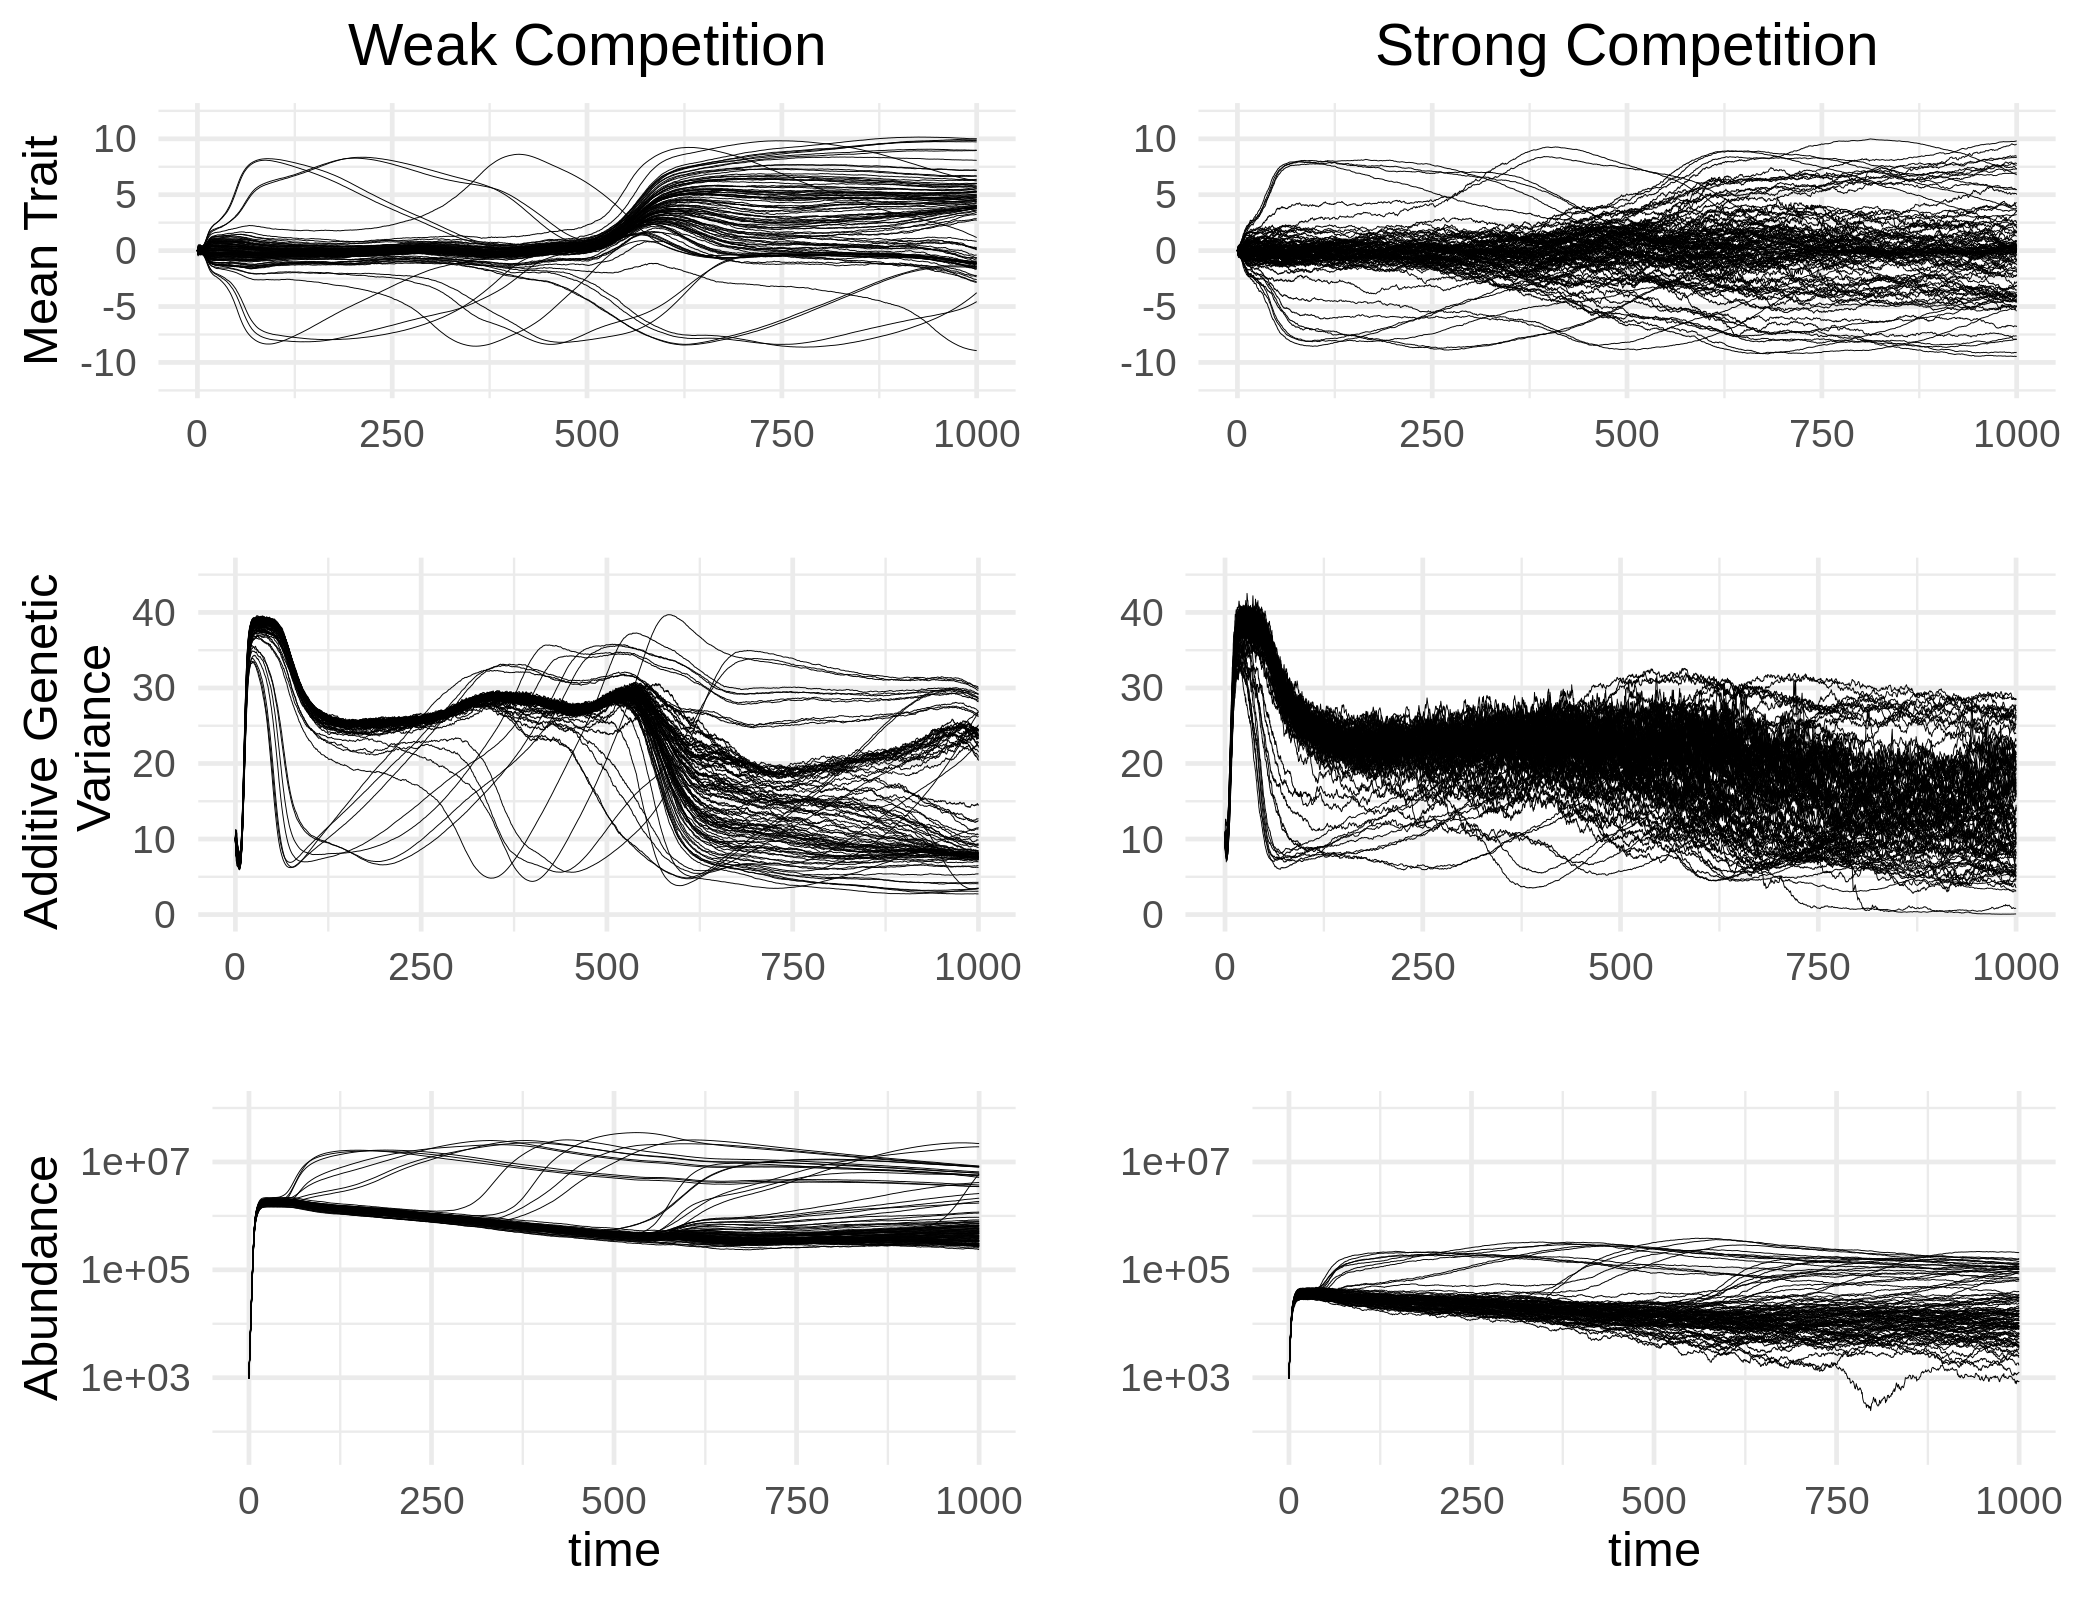
\includegraphics[width=1\linewidth]{community_dynamics} 

}

\caption{\label{temporal}Temporal dynamics of mean trait (top), additive genetic variance (middle) and abundance (bottom) for the scenario of weak competition (left) and strong competition (right).}\label{fig:unnamed-chunk-6}
\end{figure}

\hypertarget{the-relation-between-the-strength-of-ecological-interactions-and-coevolution}{%
\subsection{\texorpdfstring{The relation between the strength of
ecological interactions and coevolution
\label{ecoevo}}{The relation between the strength of ecological interactions and coevolution }}\label{the-relation-between-the-strength-of-ecological-interactions-and-coevolution}}

Relating our treatment of resource competition to modern coexistence
theory (Chesson 2000), the absolute competition coefficient
\(\alpha_{ij}\) becomes a dynamical quantity that can be written as

\begin{equation}
\alpha_{ij}(t)=\frac{c_i}{r_i(t)}\int_{-\infty}^{+\infty}\int_{-\infty}^{+\infty}p_i(x,t)p_j(y,t)\mathcal O_{ij}(x,y) dxdy =\frac{c_iU_iU_j}{r_i(t)}\sqrt\frac{b_{ij}(t)}{2\pi}\exp\left(-\frac{b_{ij}(t)}{2}\big(\bar x_i(t)-\bar x_j(t)\big)^2\right),
\end{equation}

where

\begin{equation}
r_i(t)=R_i-\frac{a_i}{2}\Big((\bar x_i(t)-\theta_i)^2+G_i(t)+\eta_i\Big).
\end{equation}

Hence, \(dN_i(t)\) can be expressed as

\begin{equation}
dN_i(t)=r_i(t)\left(1-\sum_{j=1}^S\alpha_{ij}(t)N_j(t)\right)N_i(t)dt+\sqrt{V_iN_i(t)}dW_1(t).
\end{equation}

Note that although \(r_i(t)\) is referred to in the coexistence
literature as the intrinsic growth rate of the population, \(R_i\) is a
deeper intrinsic quantity. For now we refer to \(R_i\) as the
\emph{innate} growth rate. Previous work, to list just a few citations
in this literature, has shown the importance of demographic
stochasticity (Turelli 1980; Schreiber 2017) and evolutionary dynamics
(Case and Taper 1986; Schreiber, Patel, and terHorst 2018) in
determining coexistence of competing species. However, these studies
consider evolution and demographic stochasticity separately. To our
knowledge, there are no rigorous theoretical investigations of
coexistence that account for evolutionary dynamics of quantitative
characters and demographic stochasticity simultaneously and, in
particular, no studies combining these processes that also include the
evolution of additive genetic variance. In fact, only recently have
rigorous theoretical investigations successfully combined these
processes to understand persistence of a single population
(Gomulkiewicz, Krone, and Remien 2017). Even so, these authors focused
on a single species model with a finite number of types (i.e., a
population genetic model). With the connection outlined in this section
formally established, researchers may pursue a postmodern coexistence
theory that naturally includes both the evolutionary dynamics of
quantitative characters and the effects of demographic stochasticity in
a simple synthetic framework.

In SM \S\ref{diffuse} we show that the standardized directional
selection gradient (sensu Lande and Arnold 1983) induced by species
\(j\) on species \(i\) can be computed as

\begin{equation}
\beta_{ij}(t)=c_iU_iU_jN_j(t)b_{ij}(t)\big(\bar x_i(t)-\bar x_j(t)\big) \sqrt\frac{b_{ij}(t)}{2\pi}\exp\left(-\frac{b_{ij}(t)}{2}\big(\bar x_i(t)-\bar x_j(t)\big)^2\right).
\end{equation}

Our notation differs from Lande and Arnold (1983) in that subscripts
here denote species instead of components of multivariate traits and we
drop the prime that distinguishes between selection gradients and
standardized selection gradients.

\textbf{Metric of pairwise coevolution}

Below we investigate the correspondence of interaction intensity and
coevolutionary change. However, we can already identify one major
discrepancy; \(\alpha_{ij}\) is maximized when \(\bar x_i=\bar x_j\),
but \(\beta_{ij}=0\) under the same condition. We therefore include in
our metric of selection the standardized stabilizing selection gradient
\(\gamma\) which measures the effect of stabilizing or disruptive
selection on phenotypic variance (Lande and Arnold 1983). In SM
\S\ref{diffuse} we show that the standardized stabilizing selection
gradient induced by species \(j\) on species \(i\) can be computed as

\begin{equation}
\gamma_{ij}(t)=c_iU_iU_jN_j(t)b_{ij}(t)\left(1-b_{ij}(t)\big(\bar x_i(t)-\bar x_j(t)\big)^2\right) \sqrt\frac{b_{ij}(t)}{2\pi}\exp\left(-\frac{b_{ij}(t)}{2}\big(\bar x_i(t)-\bar x_j(t)\big)^2\right).
\end{equation}

To measure the total evolutionary change in species \(i\) induced by
species \(j\), we form the metric
\(\Psi_{ij}=|\beta_{ij}|+|\gamma_{ij}|\). Figure \ref{net} displays the
joint distribution of \(\mathfrak{C}_{ij}=\Psi_{ij}\Psi_{ji}\), our
metric of pairwise coevolution, and the product of competition
coefficients \(\alpha_{ij}\alpha_{ji}\) for two simulated communities,
both with richness \(S=1000\). The solid contour represents the case of
relatively high sensitivity to competition (\(c=5\times10^{-7}\)) and
the dashed contour represents the case of relatively weak sensitivity to
competition (\(c=1\times10^{-8}\)). In both cases we see that
\(\mathfrak{C}_{ij}\) and \(\alpha_{ij}\alpha_{ji}\) are, essentially,
unrelated. However, this depiction is only representative of a specific
set of parameters. Next, we provide analytical approximations of the
covariance between selection gradients and competition coefficients and
a numerical estimate for the relationship between pairwise coevolution
and competition coefficients for a range of parameters.

\begin{figure}

{\centering 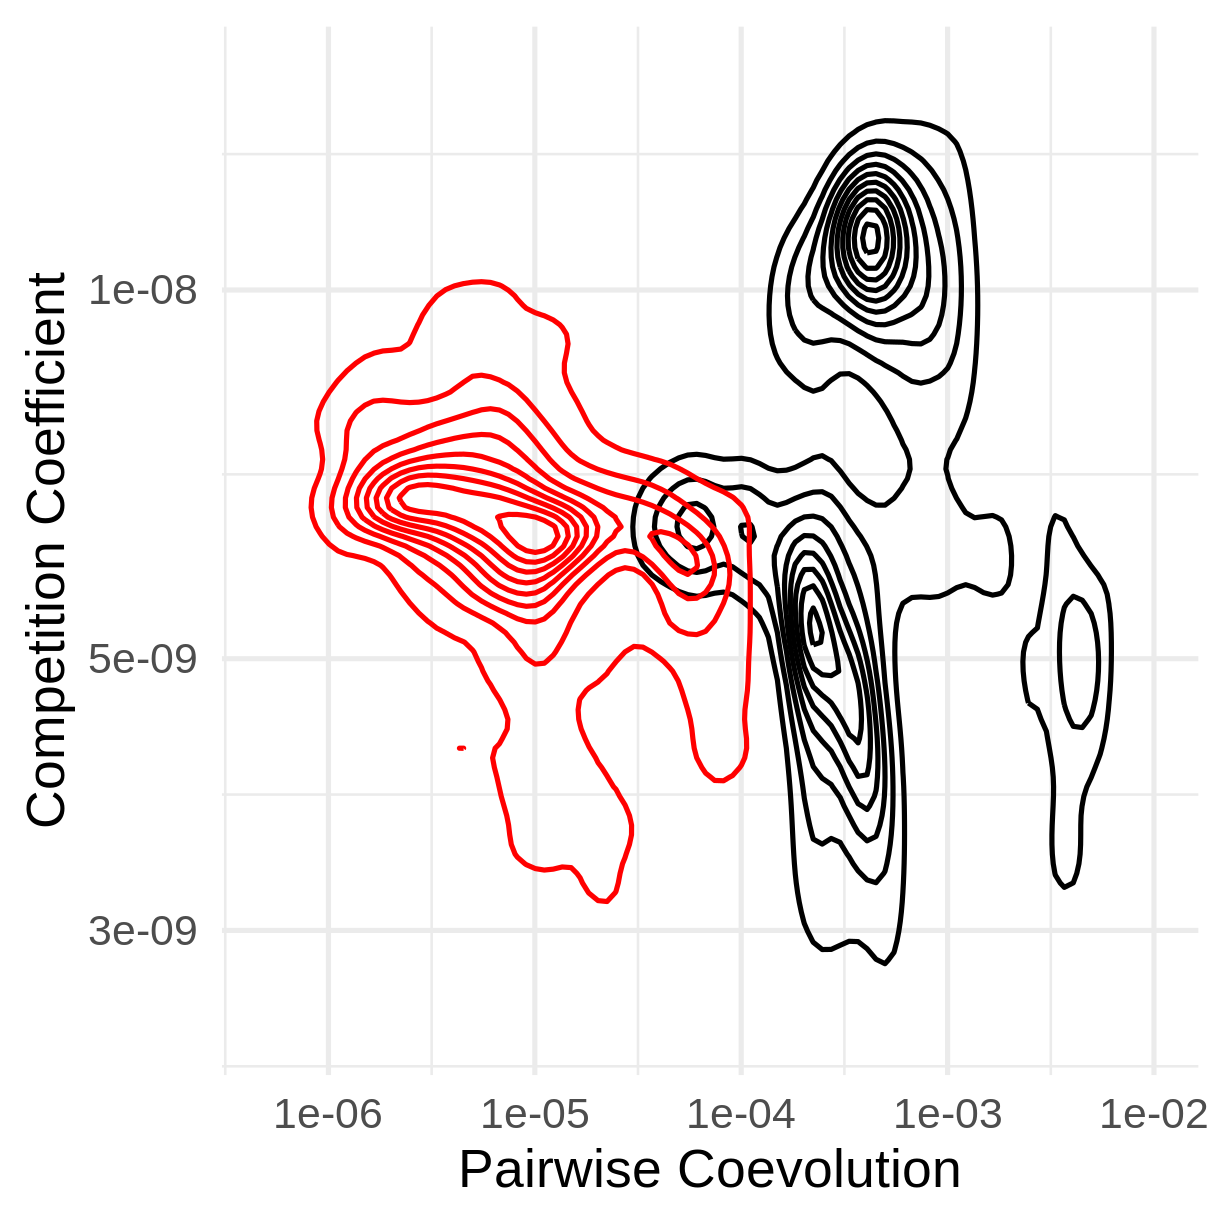
\includegraphics{on_pl} 

}

\caption{\label{net}Bivariate distributions of competition coffecients (y-axis) and pairwise coevolution (x-axis) under the scenarios of weak competition (dashed line) and strong competition (solid line) after simulating for $t=1000.0$ units of time. Simulations were ran for $S=1000$ species. Parameters are the same as in Table 2, except we used $c=1\times 10^{-8}$ for weak competition and $c=5\times 10^{-7}$ for strong competition in order to account for increased species richness.}\label{fig:unnamed-chunk-8}
\end{figure}

\textbf{Covariance of selection and competition as a function of
diversity}

We now make use of the expressions derived for competition coeffecients
and selection gradients to investigate their relationship. As a first
pass, let us assume all model parameters are equivalent across species
and that each species has the same abundance and trait variance. Let us
further assume that richness \(S\) is large and the distribution of mean
trait values is normal with mean \(\bar{\bar x}\), variance
\(V_{\bar X}\) and density \(f_{\bar X}\). Such assumptions are typical
when deriving analytical results in the field of theoretical
coevolutionary community ecology (Nuismer, Jordano, and Bascompte 2012;
Nuismer, Week, and Aizen 2018). If \(\bar{\bar x}\) is near \(\theta\)
and \(V_{\bar X}\) is much smaller than \(|2R/a-G-\eta|\), then we may
approximate \(r_i\) with

\begin{equation}
\bar r=\int_{-\infty}^{+\infty}\left(R-\frac{a}{2}\Big((\bar x-\theta)^2+G+\eta\Big)\right)f_{\bar X}(\bar x)d\bar x
=R-\frac{a}{2}\Big((\bar{\bar x}-\theta)^2+V_{\bar X}+G+\eta\Big).
\end{equation}

In SM \S\ref{coef_grad_moms} we use these assumptions to calculate the
first and second order moments describing the joint distribution of
competition coefficients and selection gradients across the community.
We find that the covariance between linear selection gradients and
competition coeffecients are zero due to the symmetry implied by our
assumptions. However, setting \(\alpha(\bar x_i,\bar x_j)=\alpha_{ij}\),
\(\beta(\bar x_i,\bar x_j)=\beta_{ij}\) and
\(\gamma(\bar x_i,\bar x_j)=\gamma_{ij}\), the covariances between the
magnitude of linear selection gradients and competition coefficients and
between stabilizing selection gradients and competition coefficients can
be written as

\begin{subequations}

\begin{equation}\label{cov_alpha_beta}
\mathrm{Cov}_{f_{\bar X}}(\alpha,|\beta|)=\frac{2c^2b^2U^4N}{\pi\bar r}\sqrt\frac{V_{\bar X}}{2\pi}\left(\frac{1}{(1+8bV_{\bar X})^{3/4}}-\frac{1}{(1+4bV_{\bar X})^{3/4}(1+2bV_{\bar X})^{1/2}}\right),
\end{equation}

\begin{equation}\label{cov_alpha_gamma}
\mathrm{Cov}_{f_{\bar X}}(\alpha,\gamma)=\frac{c^2b^2U^4N}{2\pi\bar r}(1-2bV_{\bar X})\left(\frac{1}{\sqrt{1+4bV_{\bar X}}}-\frac{1}{1+2bV_{\bar X}}\right).
\end{equation}

\end{subequations}

\begin{figure}

{\centering 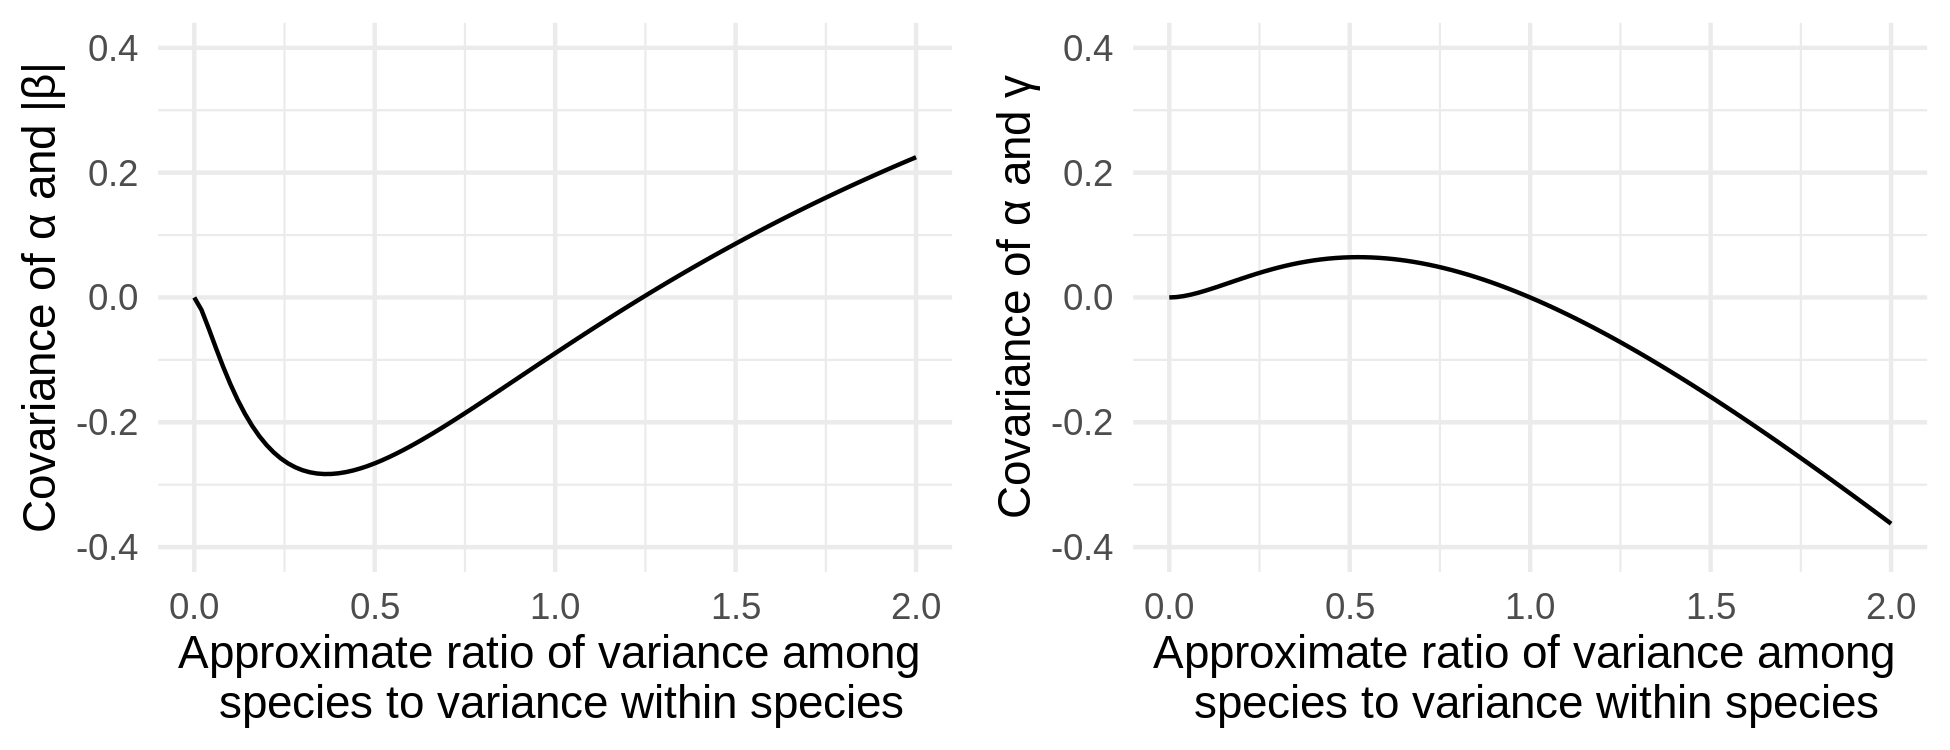
\includegraphics{/home/bb/Gits/branching.brownian.motion.and.spde/.A White Noise Approach To Evolutionary Ecology/cov} 

}

\caption{\label{cov_fig}Curves representing the covariance between the magnitude of linear selection gradients and competition coefficients (left) and between stabilizing selection gradients and competition coefficients (right) as a function of $2bV_{\bar X}$ which is approximately equal to the ratio of variance in mean traits among species to the intraspecific trait variance. In both plots we set $c=1.0\times10^{-4}$, $b=0.1$, $\bar r=0.1$ and $N=1.0\times10^{10}$ and let $V_{\bar X}$ vary.}\label{fig:unnamed-chunk-10}
\end{figure}

For fixed \(c,b,\bar r\) and \(N\), we visualize these relationships in
Figure \ref{cov_fig}. To gain insight into the relationship between
selection gradients and competition coefficients, note that our
assumptions in this section imply \(b^{-1}=2(\sigma^2+w)\). If we
further assume \(\sigma^2+w\approx\sigma^2\), then
\(2bV_{\bar X}\approx V_{\bar X}/\sigma^2\). That is, when populations
are generalists and are comprised of specialist individuals, the value
\(2bV_{\bar X}\) is approximately equal to the ratio of interspecific
mean trait variation to intraspecific individual trait variation. Hence,
for both covariances we see that there is no relationship between
selection gradients and competition coefficients when this ratio is
zero. From equation (\ref{cov_alpha_beta}) we can use numerical
optimization to find that when \(V_{\bar X}/\sigma^2\approx1.25\) the
relationship between the magnitudes of linear selection gradients and
competition coefficients disappears, but when (approximately)
\(V_{\bar X}/\sigma^2<1.25\) (\(>1.25\)), this covariance becomes
negative (positive). Equation (\ref{cov_alpha_gamma}) states that when
\(V_{\bar X}/\sigma^2\) is approximately equal to one (or slightly
larger), there is no expected relationship between competition
coefficients and quadratic selection gradients. However, when
\(V_{\bar X}/\sigma^2<1.0\) (\(>1.0\)), then we expect a positive
(negative) relationship between \(\alpha\) and \(\gamma\). These results
are true regardless of the chosen parameter values. In SM
\S\ref{coef_grad_moms} we use simulations of system
(\ref{comm_dynamics}) to show that these results do not qualitatively
differ when allowing for heterogeneous population sizes and additive
genetic variances across species.

From a biological perspective, if the ratio \(V_{\bar X}/\sigma^2\) is
small, then species are packed tightly in phenotypic space. In our model
this occurs when abiotic stabilizing selection is much stronger than
competition (\(a\gg c\)). This causes species to overlap more in niche
space (i.e., large \(\alpha\)) and creates disruptive selection for
greater intraspecific variance (i.e., positive \(\gamma\)), which
explains the positive region of covariance between \(\alpha\) and
\(\gamma\). However, as species begin to overlap in niche space,
directional selection begins to vanish (i.e., small \(|\beta|\)),
leading to a negative covariance between \(\alpha\) and \(|\beta|\). In
the limiting case that two species have perfectly overlapping niches,
they will exhibit zero directional selection since a shift in either
direction will yield the same fitness advantages.

In the opposite scenario where competition is much stronger than abiotic
stabilizing selection (\(c\gg a\)), species will not evolve to be as
tightly packed and instead their niche-centers will be spread out with
little ovelap in their resouce utilization curves (i.e., small
\(\alpha\)). In this case biotic directional selection will be strong
(i.e., large \(|\beta|\)), particularly for species towards the outer
regions of niche space due to asymmetric fitness advantages conferred by
shifts in niche-centers. This leads to a positive covariance between
\(\alpha\) and \(|\beta|\). However, as noted above, this directional
selection will also erode away at standing heritable variation (i.e.,
negative \(\gamma\)), reducing the rate at which adaptation can occur
and creating a negative covariance between \(\alpha\) and \(\gamma\).

In summary, we see the relation between competition coefficients and
selection is highly non-trivial and depends on the relative magnitudes
of different ecological processes shaping the community. However, this
does not address the relation between competition coefficients and
coevolution per se. In SM \S\ref{coef_grad_moms} we show that
calculating a formula for the covariance between competition
coefficients and the metric of coevolution \(\mathfrak{C}\) introduced
above provides a difficult analytical challenge. Instead of confronting
this challenge we build on our numerical approach used to justify
analytical approximations of
\(\mathrm{Cov}_{f_{\bar X}}(\alpha,|\beta|)\) and
\(\mathrm{Cov}_{f_{\bar X}}(\alpha,\gamma)\) to approximate the
correlation of \(\alpha\) and \(\mathfrak{C}\). This numerical approach
inherits the assumptions of homogeneous background parameters such as
the mutation rate \(\mu\) and abiotic optima \(\theta\), but allows us
to relax the assumption that \(N\) and \(G\) are constant across species
and time.

In particular, we numerically integrated system (\ref{comm_dynamics})
for \(T_1=1000.0\) units of time and then continued to integrate for
\(T_2=1000.0\) units of time. We then calculate the covariance between
the quantities \(\alpha\) and \(\mathfrak{C}\) across \(S=100\) species
for each of the last \(T_2\) time steps. We assume the temporal average
of these covariances across the last \(T_2\) units of time approximates
the expectation at equilibrium. We repeated this approach for randomly
drawn \(a\) and \(c\) until our sample size reached \(1000\). In Figure
\ref{cor_coev_fig} we plot the temporally averaged values of
\(\mathrm{Cov}_{f_{\bar X}}(\alpha,\mathfrak{C})\) against the
sensitivity to competition \(c\). Using a cubic regression, we see the
correlation of coevolutionary selection gradients and competition
coefficeints is negative at variance ratios below \(0.5\), zero at
variance ratios between \(0.5\) and \(1.0\), and drops below zero again
at variance ratios above \(1.0\).

\begin{figure}

{\centering 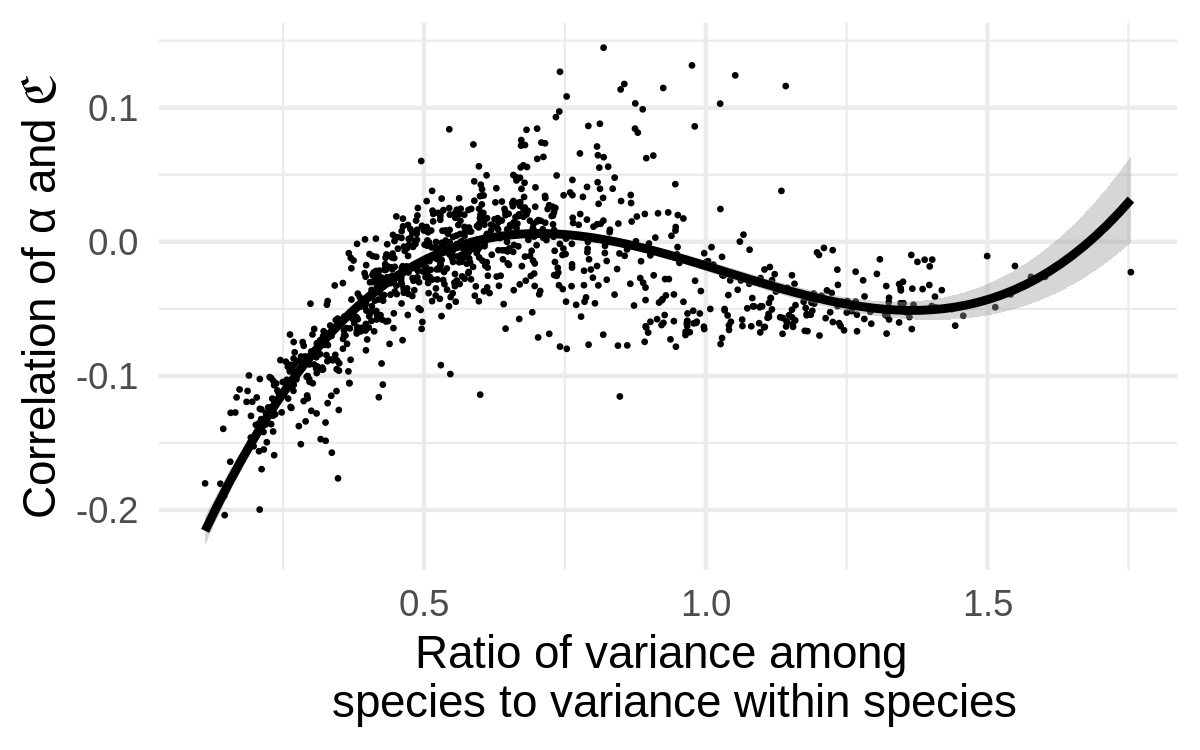
\includegraphics{/home/bb/Gits/branching.brownian.motion.and.spde/.A White Noise Approach To Evolutionary Ecology/Cαℭp} 

}

\caption{\label{cor_coev_fig}Numerical estimates for the correlation of the strength of coevolution measured by $\mathfrak{C}$ and competition coefficeints $\alpha$ plotted against the variance of mean traits among species divided by the mean variance of traits within species. Each dot represents the result from a single simulation. The red line is a cubic regression.}\label{fig:unnamed-chunk-12}
\end{figure}

\hypertarget{conclusion}{%
\section{\texorpdfstring{Conclusion
\label{conclusion}}{Conclusion }}\label{conclusion}}

We have introduced an approach to derive models of evolutionary ecology
using the calculus of white noise and coined SAGA, a SPDE model of
phenotypic evolution that accounts for demographic stochasticity. From
SAGA we derived SDE that track the evolution of abundance, mean trait
and additive genetic variance. Observing the expressions of these SDE we
find the effects of demographic stochasticity on the evolution of mean
trait and additive genetic variance characterize the effects of random
genetic drift. By considering the statistics of random samples, this has
previously been in models of fixed population size in discrete time
(Lande 1976). However, we have shown random genetic drift is a result of
demographic stochasticity for populations with fluctuating abundances in
continuous time. To illustrate the relevance of our approach to studies
of evolutionary ecology, we comined our SDE with classical competition
theory to derive a model of diffuse coevolution and used this model to
investigate the relationship between selection gradients and competition
coefficients. This work demonstrates that connecting contemporary
theoretical approaches to evolutionary ecology with some fundamental
results in the theory of measure-valued stochastic processes allows for
the development of a rigorous, yet flexible approach to synthesizing the
dynamics of abundance and distributions of quantitative characters, in
agreement with Champagnat, Ferrière, and Méléard (2006). Although this
approach enjoys these important merits, there remains biological details
and their associated technical challenges that need to be confronted for
gaining a more thorough and accurate understanding of ecological
communities. We touch on just four of them here and provide suggestions
for future research to approach these challenges. For the first three,
we recommend the use of individual-based simulations of measure-valued
processes to confront these challenges. To summarize why, we state here
that analytical results become difficult to derive for small populations
and complicated models of mutation and selection.

\textbf{Limitations of diffusion limits and generalizing coexistence
theory}

As noted by Feller (1951), diffusion limits provide reasonable
approximations for large populations, but relatively small populations
require discrete models. Hence, as a diffusion limit, SPDE (\ref{SPDE})
restricts parameter values to regions that maintain large population
sizes. Although this suggests an important restriction on any model
developed under this framework by implying populations are not at risk
of extinction, the SDE describing abundance dynamics technically permits
extinction. However, for small abundances, pathology emerges in the
evolution of trait means and variances. In particular, stochastic
components of the SDE describing the evolution of \(\bar x\) and
\(\sigma^2\) diverge towards infinite values as \(N\to0\). Hence,
studies involving extinction and phenotypic evolution should be pursued
through a different approach. A natural alternative can be developed
utilizing the underlying measure-valued branching process that SAGA is a
diffusion limit of (see section \ref{stochastic}). This process
explicitly tracks individuals throughout their life-history and captures
reproduction as branching events. Hence, branching processes model
population size as a non-negative integer instead of a continuously
varying number. In particular, the pathological behavior described for
the SDE of \(\bar x\) and \(\sigma^2\) does not occur for measure-valued
branching processes. This concern relates to our comment in
\S\ref{ecoevo} on using our model of diffuse coevolution to extend
modern coexistence theory (sensu Chesson 2000) in a way that accounts
for phenotypic evolution and demographic stochasticity. Just as previous
work has sought to understand the implications of processes for
coexistence separately, it seems necessary to determine whether or not
results pertaining to the coexistence of competing populations hold
using models that account for phenotypic evolution and demographic
stochasticity simultaneously. Because such investigations consider both
extinction and phenotypic evolution we argue the models used should be
either simulations of, or whenever possible, analytical results based on
measure-valued branching processes.

\textbf{The genetic architecture and distributions of traits}

Our treatment of inheritance and our approach to model coevolution rests
on the assumptions of normally distributed breeding values and expressed
phenotypes along with asexual reproduction. However, real traits are not
encoded by an infinite number of loci each contributing an additive
infinitesimal effect (as required by the infinitesimal model), mutations
are not inherited as normally distributed deviations from parental
breeding values (as required by the Gaussian allelic model) and many
populations of interest exhibit non-random sexual reproduction.
Departures from this model of genetic architecture can produce more
complex distributions of breeding values and expressed traits. Such
deviations can be reinforced via strong non-Gaussian selection surfaces,
including the surface \(m(\nu,x)\) we have derived from niche theory,
along with non-random mating in sexually reproducing populations.
However, Gaussian approximations are convenient since they are defined
by their mean and variance. Future work investigating the effects of
non-normally distributed traits on the structure and dynamics of
ecological communities will therefore need to confront higher moments
such as skew and kurtosis, ideally integrating previously established
mathematical approaches to derive the dynamics of these higher moments
(Débarre, Yeaman, and Guillaume 2015).

Another approach to breaking the assumption of normally distributed
trait values is the development of explicit multilocus models. These
models describe the contributions of alleles at particular loci in the
genome to the development of quantitative traits. Tracking the
fluctuations of allele frequencies then allows theoreticians to
investigate the dynamics of phenotypic distributions that deviate from
normality. This approach has a long history in theoretical quantitative
genetics (Bulmer 1980; Turelli and Barton 1994; Kirkpatrick, Johnson,
and Barton 2002) and coevolutionary theory (Nuismer, Doebeli, and
Browning 2005; Kopp and Gavrilets 2006; Nuismer, Ridenhour, and Oswald
2007). However, work to investigate the role of complex genetic
architectures in mediating feedbacks between the dynamics of population
abundances and the distributions of traits mediating ecological
interactions has apparently only just begun (Patel and Bürger 2019).
Since analytical results are difficult to obtain for general models of
mutation, development and selection (c.f., Bürger 2000), we again
suggest the use of measure-valued branching processes and their
individual-based simulations. For example, by assuming the mutational
effects in the BBM model is Gaussian with variance an order of magnitude
greater than the equilibrium phenotypic (or genetic) variance, we obtain
the so-called \emph{House-of-cards} model (Turelli 1984). However,
perhaps considering heavy-tailed distributions, such as the
Laplace-distributions considered in Park et. al. (2017), will provide
more realistic, yet less analytically tractable models of mutational
effects. Such models have important implications in conservation
genetics where small populations may evolve primarily in response to
mutation and random genetic drift (Lande 1995).

\textbf{Ecological stoichiometry}

Our treatment of both biotic and abiotic selection neglects important
chemical constraints of biological reality. For instance, the resource
we assume species are competing over is modelled as a static quantity.
However, real resources can be dynamic quantities. Such theoretical
quantities may reflect abiotic cycles of material and energy or whole
trophic layers comprised of prey, hosts or mutualists. Although resource
dynamics have been captured theoretically in consumer-resource models
(Tilman 1982), developing a more realistic model of resource competition
must incorporate details on the ecophysiology of organisms (Loreau
2010). Doing so will help clarify the feedback between the evolution of
populations and the ecosystem processes they are a part of.

Using plant-pollinator communities as an example, the role of nitrogen
mediating interspecific interactions has been reviewed by David, Storkey
and Stevens (2019) and the evolutionary ecology of the nutritional
content of nectar has been reviewed by Parachnowitsch, Manson and
Sletvold (2018). These studies demonstrate the need for further research
to understand how soil nutrient availability and organismal
ecophysiology structures communities of plants and pollinators.
Theoretical pursuits in this direction may profit from interfacing the
framework we have outlined here with population-ecosystem models such as
that developed by Fridley (2017). However, these population-ecosystem
models will likely yield complicated fitness functions that are
difficult to analyze using rigorous mathematical techniques. Hence, we
again recommend the use of simulations of measure-valued branching
processes that generalize BBM to understand when analytical
approximations hold.

\textbf{Accounting for macroevolutionary history}

To understand patterns found in ecological communities, considerations
must push beyond microevolutionary and contemporary ecological processes
and consider the macroevolutionary dynamics of ancestral lineages
leading to extant populations. Using sub-alpine flower communities as an
example, one can observe a very strict ordering of phenology across a
broad geographic range. In particular, whether in the Colorado Rocky
mountains (such as Gothic, Colorado) or on an outlier of the Idaho
batholith (such as Kamiak butte near Palouse, Washington), one will
almost surely observe a very conspicuous order of flowers emerging in
early spring: at the very beginning of the season blooms \emph{Claytonia
lanceolata} followed by \emph{Erythronium grandiflorum} which precedes
\emph{Delphinium nuttallianum} (B. Week, personal observations). If
contemporary phenological coevolution is rampant, why should this
pattern be so well preserved across a thousand miles of rugged and
diverse terrain? Although it would be exciting to find that these
species repeatedly coevolved this pattern in each location, a more
parsimoniuous hypothesis suggests the phenology and physiology of these
species slowly evolved independently over macroevolutionary time scales
to take advantage of the specific conditions available within each of
these windows of the flowering season. However, this could not have
carried out in the Rocky mountains since this terrain only became
habitable just over ten thousand years ago as the glaciers of the
Pleistocene began to retreat (Paul CaraDonna, personal communications).
Hence, given these considerations, it appears that an understanding of
early season phenology patterns should focus on how these communities
are assembled as opposed to contemporary evolutionary dynamics. Indeed,
recent work testing models of phylogeography ignores the potential for
contemporary evolution and instead suggests alpine flower communities
tend to follow neutral assembly where flowers merely compete for who can
disperse to new habitat first, as opposed to a selective process where a
regional species pool is filtered for those species adapted to the newly
available habitat (Marx et al. 2017).

Of course microevolutionary and ecological dynamics are not completely
irrelevant for understanding patterns in communities that are primarily
structured by deep evolutionary processes. In particular,
macroevolutionary trait evolution is simply the aggregation of
microevolutionary change occuring over large spans of time. This
suggests a road forward to connect the theory we have introduced to
models of macroevolutionary trait evolution.

Some approaches to modelling macroevolutionary trait change simply
repurpose microevolutionary models by blindly rescaling time from the
units of generations to millions of years {[}Nuismer and Harmon (2014);
Luke, can you think of others?{]}. Such an approach makes the implicit
assumption that trait evolution is statistically self-similar (sensu
Falconer 2014) so that the stochastic evolution of traits on
macroevolutionary time scales has the same properties of trait evolution
on microevolutionary time scales. Although some stochastic processes,
including Brownian motion, do exhibit self-similarity, others do not.
For example, consider a modification of the Ornstein-Uhlenbeck process
defined by the SDE

\begin{equation}
dX_t=a(\theta_t-X_t)dt+bdW_t
\end{equation}

where \(a,b>0\), \(W_t\) is a standard Brownian motion and \(\theta_t\)
is itself a Markov process that takes normally distributed jumps
centered on its current location at exponentially distributed time
intervals. If we assume the rate \(\lambda\) at which jumps occur is
much smaller than \(a\) and the variance in jumping is much larger than
\(b^2\), then, even though the sample paths of \(X_t\) are actually
continuous (if we zoom in close enough, they look like Brownian motion),
over long intervals of time sample paths of \(X_t\) will begin to appear
to have periods of continuity interrupted by an occasional discontinuous
jump and thus approach a qualitatively distinct process. These emergent
properties can be formally characterized by Lévy processes and have been
successfully employed in comparative phylogenetics to fit phenotypic
data from extant populations and the fossil record (Landis and Schraiber
2017). It would therefore be interesting to investigate whether an
application of a separation of time scales argument for the rate of
environmental change (\(\lambda\)) versus the rate of evolutionary and
ecological change (\(a\)) to microevolutionary models derived using our
framework can be used to obtain macroevolutionary models that include
not only mean trait evolution, but also the evolution of trait variance
and abundance. The resulting macroevolutionary models can give rise to
novel comparative phylogenetic methods and provide initial conditions
for microevolutionary models that capture contemporary dynamics.

\textbf{Final remarks}

Although top-down approaches to community ecology, such as the Maximum
Entropy Theory of Ecology (Harte 2011), have enjoyed some success in
describing community-level patterns (Harte and Newman 2014; Xiao,
McGlinn, and White 2015), a mechanistic understanding of why these
patterns emerge and how they will change remains a formidable task. Such
an understanding must take both bottom-up and top-down approaches
integrating considerations from the ecophysiology of individual
organisms that reveal the economics of interspecific interactions
(Sterner and Elser 2008), to the phylogeographic history of taxa that
sets the stage for contemporary dynamics (Hickerson et al. 2010).
Through connecting these dots we can increase the variance explained in
observations of ecological communities by specific mechanisms and come
closer to a predictive theory of evolutionary community ecology. Despite
the long list of equations derived in this paper, this work takes just
one small step towards capturing these many details. However, we hope
the theoretical framework outlined here along with the demonstration of
its use in modelling competitive communities provides some helpful tools
to aid quantitative evolutionary ecologists in reaching such lofty
goals.

\newpage

\hypertarget{supplementary-material-sm}{%
\section{Supplementary material (SM)}\label{supplementary-material-sm}}

Throughout this supplement, we set use dot notation for time derivatives
so that \(\dot f(x,t)=\frac{\partial }{\partial t}f(x,t)\) and set
\(\Delta=\sum_{i=1}^d\frac{\partial^2}{\partial x_i^2}\) the Laplace
operator on \(\mathbb{R}^d\), except in \S\ref{caC} where \(\Delta\)
represents a random variable.

\hypertarget{sufficient-conditions-for-finite-mean-variance-and-total-abundance-in-the-deterministic-case}{%
\subsection{\texorpdfstring{Sufficient conditions for finite mean,
variance and total abundance in the deterministic case
\label{finite}}{Sufficient conditions for finite mean, variance and total abundance in the deterministic case }}\label{sufficient-conditions-for-finite-mean-variance-and-total-abundance-in-the-deterministic-case}}

Recall that \(m(\nu,x)\) is shorthand for \(m\big((K\nu)(x,t),x\big)\).
That is, \(m:[0,+\infty)\times\mathbb{R}\to\mathbb{R}\). Following our
assumptions of the main text, we have that \(m(h,x)\) is differentiable
with respect to both \(x\) and \(h\) and there exists \(r\in\mathbb{R}\)
such that \(m(h,x)\leq r\) across all \(h\geq0\) and \(x\in\mathbb{R}\).
As in the main text, we also assume the initial condition \(u(x)\) is
continuous and integrable in \(x\) and satisfies \begin{equation}
0\leq\int_{\mathbb{R}}(|x|+x^2)u(x)dx<+\infty
\end{equation} and consider the Cauchy problem
\begin{equation}\label{PDE_SM}
\left\{\begin{matrix}
\dot\nu(x,t)=m(\nu,x)\nu(x,t)+\frac{\mu}{2}\Delta\nu(x,t) & t>0\\
\nu(x,0)=u(x) & t=0.
\end{matrix}\right.
\end{equation}

According to Theorem 2.5.6 of Zheng (2004), if the operator \(F\)
defined by \(\nu(x,t)\to m(\nu,x)\nu(x,t)\) is locally Lipschitz,
corresponding to equation (\ref{local_lipschitz}) of the main text, then
for some maximal \(T>0\) problem (\ref{PDE_SM}) admits a unique local
classical solution \(\nu(x,t)\) for \(t\in[0,T)\). Furthermore, either
\(T=+\infty\) or \(T<+\infty\) and
\(\lim_{t\uparrow T}\int_\mathbb{R}|\nu(x,t)|dx=+\infty\). In this
section we show that our assumption \(m(h,x)\leq r\) for all \(h\geq0\)
and \(x\in\mathbb{R}\) implies \(T=+\infty\). Replacing \(m\) with it's
upper bound \(r\in\mathbb{R}\), equation (\ref{PDE_SM}) reduces to a
simple parabolic equation that can be solved using elementary techniques
(Farlow 1993). In particular, when \(m(\nu,x)\equiv0\) denote the
solution to (\ref{PDE_SM}) by \(\nu_0(x,t)\). Then, denoting
\begin{equation}
\Phi(x,t)=\frac{\exp\left(-x^2/2\mu t\right)}{\sqrt{2\pi\mu t}},
\end{equation} we have \begin{equation}
\nu_0(x,t)=\int_{\mathbb{R}}\Phi(x-y,t)\nu(y,0)dy.
\end{equation} In the more general case, when
\(m(\nu,x)\equiv r\in\mathbb{R}\), equation (\ref{PDE_SM}) has the
solution \(\nu_r(x,t)=e^{rt}\nu_0(x,t)\). Hence, \(\nu_r(x,t)\geq0\) for
all \(x\in\mathbb{R}\) and
\(\int_\mathbb{R}\nu_r(x,t)dx=e^{rt}N(0)<+\infty\) for all \(t\geq0\).
Furthermore, denoting \begin{equation}
\begin{matrix}
N_r(t)&=&\int_\mathbb{R}\nu_r(x,t)dx, \\
p_r(x,t)&=&\nu_r(x,t)/N_r(t), \\
\bar x_r(t)&=&\int_\mathbb{R}xp_r(x,t)dx, \\
\sigma^2_r(t)&=&\int_\mathbb{R}(x-\bar x_r(t))^2p_r(x,t)dx, 
\end{matrix}
\end{equation} we have \begin{equation}
\bar x_r(t)=\int_\mathbb{R}x\int_\mathbb{R}\Phi(x-y,t)p(y,0)dydx=\int_\mathbb{R}yp(y,0)dy=\bar x(0),
\end{equation} \begin{equation}
\sigma_r^2(t)=\int_\mathbb{R}(x-\bar x_r(t))^2\int_\mathbb{R}\Phi(x-y,t)p(y,0)dydx=\int_\mathbb{R}\Big((y-\bar x(0))^2+\mu t\Big)p(y,0)dy=\sigma^2(0)+\mu t.
\end{equation} Hence, \(|\bar x_r(t)|,\sigma_r^2(t)<+\infty\) for all
\(t\geq0\). For the sake of contradiction, suppose there exists
\(x\in\mathbb{R}\) and \(t\geq0\) such that \(\nu(x,t)>\nu_r(x,t)\).
Then \begin{equation}
\nu(x,t)-\nu(x,0)=\int_0^tm(\nu,x)\nu(x,s)+\frac{\mu}{2}\Delta\nu(x,s)ds>\int_0^tr\nu_r(x,s)+\frac{\mu}{2}\Delta\nu_r(x,s)ds=\nu_r(x,t)-\nu(x,0)
\end{equation} which implies there exists \(h\geq0\) and
\(x\in\mathbb{R}\) such that \(m(h,x)>r\). But this contradicts our
assumption \(m(h,x)\leq r\) for all \(h\geq0\) and \(x\in\mathbb{R}\).
So we have \(\nu(x,t)\leq\nu_r(x,t)\) for each \(x\in\mathbb{R}\) and
\(t\geq0\). This implies that
\(N(t)=\int_\mathbb{R}\nu(x,t)dx<+\infty\), \begin{equation}
0\leq\int_\mathbb{R}x^2\nu(x,t)dx\leq\int_\mathbb{R}x^2\nu_r(x,t)dx<+\infty
\end{equation} and in particular \begin{equation}
0\leq\sigma^2(t)+\bar x^2(t)=\frac{1}{N(t)}\int_\mathbb{R}x^2\nu(x,t)dx<+\infty
\end{equation} for each \(t\geq0\).

\hypertarget{equilibrium-moments-for-a-deterministic-population-experiencing-logistic-growth-and-stabilizing-selection}{%
\subsection{\texorpdfstring{Equilibrium moments for a deterministic
population experiencing logistic growth and stabilizing selection
\label{equilib}}{Equilibrium moments for a deterministic population experiencing logistic growth and stabilizing selection }}\label{equilibrium-moments-for-a-deterministic-population-experiencing-logistic-growth-and-stabilizing-selection}}

Here we set out to show, given the initial conditions
\(\nu(\cdot,0)\in L^1(\mathbb{R})\) such that
\(\bar x(0)\in\mathbb{R}\), \(\sigma^2(0)\in[0,+\infty)\) and
\(N(0)\in(0,+\infty)\), and given the growth rate
\begin{equation}\label{m_log_stab}
m(\nu,x)=r-\frac{a}{2}(\theta-x)^2-c\int_\mathbb{R}\nu(y,t)dy
\end{equation} such that \(\theta\in\mathbb{R}\), \(a,c,\mu>0\) and
\(r>\tfrac{1}{2}\sqrt{\mu a}\), we have the following stable equilibrium
\(N_\infty=\lim_{t\to\infty}N(t)=\tfrac{1}{c}(r-\tfrac{1}{2}\sqrt{a\mu})\),
\(\bar x_\infty=\lim_{t\to\infty}\bar x(t)=\theta\) and
\(\sigma^2_\infty=\lim_{t\to\infty}\sigma^2(t)=\sqrt{\tfrac{\mu}{a}}\).

The mean fitness can be calculated as \begin{equation}
\bar m(t)=r-\frac{a}{2}((\theta-\bar x(t))^2+\sigma^2(t))-cN(t).
\end{equation} Recalling the ODE derived for \(N(t)\), \begin{equation}
\frac{d}{dt}N(t)=\bar m(t)N(t)=(r-\frac{a}{2}((\theta-\bar x(t))^2+\sigma^2(t))-cN(t))N(t),
\end{equation} solving for equilibrium total abundance \(\hat N\)
amounts to setting \(\frac{d}{dt}N(t)=0\) and solving for \(N(t)\).
Ignoring the equilibrium \(N(t)=0\), this reduces to solving
\(\bar m(t)=0\) for \(N(t)\), which returns \begin{equation}
\hat N=\frac{1}{c}\left(r-\frac{a}{2}\left((\theta-\hat{\bar x})^2-\hat\sigma^2\right)\right).
\end{equation} Unfortunately, deriving ODE for \(\bar x(t)\) and
\(\sigma^2(t)\) leads to expressions involving higher moments and
finding ODE for these higher moments will lead to expressions involving
yet even higher moments. To avoid this infinite regression, we find the
equilibrium abundance density \(\hat\nu(x)\) by solving
\(\frac{\partial}{\partial t}\nu(x,t)=0\) for \(\nu(x,t)\). This implies
the following ordinary differential equation \begin{equation}
\frac{d^2}{dx^2}\hat\nu(x)=\left(\frac{2c}{\mu}\hat N+\frac{a}{\mu}(\theta-x)^2-\frac{2r}{\mu}\right)\hat\nu(x)
\end{equation} which has the solution \begin{equation}
\hat\nu(x)=\frac{\hat N}{\sqrt{2\pi}}\left(\frac{a}{\mu}\right)^{\frac{1}{4}}\exp\left(-\sqrt\frac{a}{\mu}\frac{(\theta-x)^2}{2}\right).
\end{equation} From this expression we infer \(\hat{\bar x}=\theta\) and
\(\hat\sigma^2=\sqrt{\frac{\mu}{a}}\). Hence
\(\hat N=\frac{1}{c}\left(r-\frac{1}{2}\sqrt{a\mu}\right)\). To show
that \(N_\infty=\hat N\), \(\bar x_\infty=\hat{\bar x}\) and
\(\sigma^2_\infty=\hat\sigma^2\), we linearize ODE for \(N(t)\),
\(\bar x(t)\) and \(\sigma^2(t)\) using the equilibrium \(\hat\nu(x)\).
In particular, since \(\hat\nu(x)\) is Gaussian, we do not run into the
same issue with higher moments as above. Assuming the equilibrium
\(\hat\nu(x)\) does not change the ODE for \(N(t)\), but the ODE for
\(\bar x(t)\) and \(\sigma^2(t)\) can now be expressed as
\begin{equation}
\frac{d}{dt}\bar x(t)=\sigma^2(t)\left(\frac{\partial\bar m(t)}{\partial\bar x(t)}-\overline{\frac{\partial m(t)}{\partial\bar x(t)}}\right)=a\sigma^2(t)(\theta-\bar x(t)),
\end{equation} \begin{equation}
\frac{d}{dt}\sigma^2(t)=2\sigma^4(t)\left(\frac{\partial\bar m(t)}{\partial\sigma^2(t)}-\overline{\frac{\partial m(t)}{\partial\sigma^2(t)}}\right)+\mu=\mu-a\sigma^4(t),
\end{equation} where \(\hat p(x)=\hat\nu(x)/\hat N\). These expressions
confirm our findings that \(\hat{\bar x}=\theta\) and
\(\hat\sigma^2=\sqrt{\frac{\mu}{a}}\). Furthermore, calculating
\begin{equation}
\frac{\partial}{\partial\sigma^2(t)}\frac{d}{dt}\sigma^2(t)=-2a\sigma^2(t)
\end{equation} and evaluating at \(\sigma^2(t)=\hat\sigma^2\)
demonstrates the equilibrium phenotypic variance is stable when
\(a,\mu>0\). Hence, calculating \begin{equation}
\frac{\partial}{\partial\bar x(t)}\frac{d}{dt}\bar x(t)=-a\sigma^2(t)
\end{equation} and evaluating at \(\sigma^2(t)=\hat\sigma^2\) and
\(\bar x(t)=\hat{\bar x}\) demonstrates the equilibrium phenotypic mean
is stable when \(a,\mu>0\). Finally, calculating \begin{equation}
\frac{\partial}{\partial N(t)}\frac{d}{dt}N(t)=r-\frac{a}{2}((\theta-\bar x(t))^2+\sigma^2(t))-2cN(t)
\end{equation} and evaluating at \(\sigma^2(t)=\hat\sigma^2\),
\(\bar x(t)=\hat{\bar x}\) and \(N(t)=\hat N\) demonstrates the
equilibrium total abundance is stable when \(a,c,\mu>0\), and
\(r>\frac{1}{2}\sqrt{a\mu}\).

\hypertarget{the-relation-between-diffusion-and-convolution-with-a-gaussian-kernel}{%
\subsection{\texorpdfstring{The relation between diffusion and
convolution with a Gaussian kernel
\label{diffconvequiv}}{The relation between diffusion and convolution with a Gaussian kernel }}\label{the-relation-between-diffusion-and-convolution-with-a-gaussian-kernel}}

For continuous \(g:\mathbb{R}^d\to\mathbb{R}\), consider the
deterministic Cauchy problem \begin{equation}\label{heateqn}
\left\{\begin{matrix}
\dot f(x,t)=&\Delta f(x,t), & (x,t)\in\mathbb{R}^d\times(0,\infty)\\
f(x,t)=&g(x), & (x,t)\in\mathbb{R}^d\times\{0\}.
\end{matrix}\right.
\end{equation} According to Evans (2010), the fundamental solution of
(\ref{heateqn}) is \begin{equation}
\Phi(x,t)=\frac{1}{(4\pi t)^{d/2}}\exp\left(-\frac{|x|^2}{4t}\right), \ (x,t)\in(0,\infty)\times\mathbb{R}^d,
\end{equation} where \(|x|=\sqrt{\sum_ix_i^2}\). The solution \(f(x,t)\)
of PDE (\ref{heateqn}) is then given by the convolution \begin{equation}
f(x,t)=\int_{\mathbb{R}^d}\Phi(x-y,t)g(y)dy, \ (x,t)\in(0,\infty)\times\mathbb{R}^d.
\end{equation} Hence, by the fundamental theorem of calculus,

\begin{multline}
f(x,t)+\int_t^{t+1}\dot f(x,s)ds=f(x,t+1) \\
=\int_{\mathbb{R}^d}\Phi(x-y,t+1)g(y)dy=\int_{\mathbb{R}^d}\int_{\mathbb{R}^d}\Phi(x-y,1)\Phi(y-z,t)g(z)dzdy \\
=\int_{\mathbb{R}^d}\Phi(x-y,1)f(t,y)dy.
\end{multline} In particular, \begin{equation}
f(x,t)+\int_t^{t+1}\Delta f(x,s)ds=\int_{\mathbb{R}^d}\Phi(1,x-y)f(y,t)dy.
\end{equation}

\hypertarget{deterministic-dynamics-of-sigma2t}{%
\subsection{\texorpdfstring{Deterministic dynamics of \(\sigma^2(t)\)
\label{var_deriv}}{Deterministic dynamics of \textbackslash{}sigma\^{}2(t) }}\label{deterministic-dynamics-of-sigma2t}}

Picking up from the main text \S\ref{deterministic},

\begin{multline}
\frac{d}{dt}\sigma^2(t)=\frac{d}{dt}\int_\mathbb{R}(x-\bar x(t))^2p(x,t)dx=\int_\mathbb{R}2(x-\bar x(t))\frac{d}{dt}{\bar x}(t)+(x-\bar x(t))^2\frac{\partial}{\partial t} p(x,t)dx\\=\int_\mathbb{R}(x-\bar x(t))^2\left((m(\nu,x)-\bar m(t))p(x,t)+\frac{\mu}{2}\frac{\partial^2}{\partial x^2}p(x,t)\right)dx\\=\int_\mathbb{R}\left((x-\bar x(t))^2-\sigma^2(t)+\sigma^2(t)\right)(m(\nu,x)-\bar m(t))p(x,t)+(x-\bar x(t))^2\frac{\mu}{2}\frac{\partial^2}{\partial x^2}p(x,t)dx\\=\mathrm{Cov}_t\Big((x-\bar x(t))^2,m(\nu,x)\Big)+\frac{\mu}{2}\int_\mathbb{R}(x-\bar x(t))^2\frac{\partial^2}{\partial x^2}p(x,t)dx.
\end{multline} Applying integration by parts twice yields
\begin{equation}
\int_{-\infty}^{+\infty}(x-\bar x(t))^2\frac{\partial^2}{\partial x^2}p(x,t)dx=2.
\end{equation}

\hypertarget{simplifying-covariances-with-fitness-under-the-assumption-of-a-gaussian-density}{%
\subsection{\texorpdfstring{Simplifying covariances with fitness under
the assumption of a Gaussian density
\label{cov2deriv}}{Simplifying covariances with fitness under the assumption of a Gaussian density }}\label{simplifying-covariances-with-fitness-under-the-assumption-of-a-gaussian-density}}

By assuming

\begin{equation}
p(x,t)=\frac{\exp\left(-\frac{(x-\bar x(t))^2}{2\sigma^2(t)}\right)}{\sqrt{2\pi\sigma^2(t)}}
\end{equation}

we have

\begin{multline}
\sigma^2\left(\frac{\partial\bar m}{\partial\bar x}-\overline{\frac{\partial m}{\partial\bar x}}\right)=\sigma^2\left(\frac{\partial}{\partial\bar x}\int_\mathbb{R}m(\nu,x)p(x,t)dx-\int_\mathbb{R}p(x,t)\frac{\partial}{\partial \bar x}m(\nu,x)dx\right)\\=\sigma^2\int_\mathbb{R}m(\nu,x)\frac{\partial}{\partial\bar x}p(x,t)dx=\sigma^2\int_\mathbb{R}\frac{x-\bar x(t)}{\sigma^2}m(\nu,x)p(x,t)dx\\=\int_\mathbb{R}(x-\bar x)(m(\nu,x)-\bar m)p(x,t)dx=\mathrm{Cov}_t(m,x),
\end{multline}

and

\begin{multline}
2\sigma^4\left(\frac{\partial\bar m}{\partial\sigma^2}-\overline{\frac{\partial m}{\partial\sigma^2}}\right)=2\sigma^4\left(\frac{\partial}{\partial\sigma^2}\int_\mathbb{R}m(\nu,x)p(x,t)dx-\int_\mathbb{R}p(x,t)\frac{\partial}{\partial\sigma^2}m(\nu,x)dx\right)\\=2\sigma^4\int_\mathbb{R}\frac{(x-\bar x)^2-\sigma^2}{2\sigma^4}m(\nu,x)p(x,t)dx=\int_\mathbb{R}\left((x-\bar x)^2-\sigma^2\right)\big(m(\nu,x)-\bar m\big)p(x,t)dx\\=\mathrm{Cov}_t\Big((x-\bar x)^2,m\Big).
\end{multline}

\hypertarget{comparing-our-treatment-of-white-noise-to-da-prato-and-zabczyk-2014}{%
\subsection{\texorpdfstring{Comparing our treatment of white noise to Da
Prato and Zabczyk (2014)
\label{DPZ14}}{Comparing our treatment of white noise to Da Prato and Zabczyk (2014) }}\label{comparing-our-treatment-of-white-noise-to-da-prato-and-zabczyk-2014}}

Our approach in the main text is inspired by the treatment provided in
\S4.2 of Da Prato and Zabczyk (2014). Here the authors develop a
stochastic integral of operator-valued processes. In particular, they
consider processes indexed by time \(t\geq0\) valued as Hilbert-Schmidt
operators \(\Phi(t)\) and define the norm \begin{equation}
\|\Phi\|_t=\sqrt{\mathbb{E}\left(\int_0^t\mathrm{Tr}[\Phi(s)\Phi^*(s)]ds\right)}, \ t\geq0.
\end{equation} In our case we only consider the so-called multiplication
operators. That is, processes that consist of operators \(\Phi(t)\)
having the form \(\Phi(t)g(x)=\varphi(x,t)g(x)\) such that
\(\varphi(\cdot,t)\in L^2(\mathbb{R})\) a.s. for each \(t\geq0\). In
this case \(\Phi(t)=\Phi^*(t)\) and \begin{equation}
\|\Phi\|_t=\|\varphi\|_t=\sqrt{\mathbb{E}\left(\int_0^t\int_\mathbb{R}\varphi^2(x,s)dxds\right)}, \ t\geq0.
\end{equation} Da Prato and Zabczyk (2014) form the space
\(\mathscr{N}^2_W(0,T)\) of Hilbert-Schmidt operator-valued predictable
processes \(\Phi(t)\) that satisfy \(\|\Phi\|_T<+\infty\) for some
\(T>0\). This corresponds to our more specialized space
\(\mathscr{N}_2\) that consists of \(L^2(\mathbb{R})\) valued processes
\(\varphi(x,t)\) such that \(\|\varphi\|_t<+\infty\) for all \(t\geq0\).
In their treatment, \(W(t)\) plays a similar role to our generalized
process \(\mathbf{W}_t\). For \(\Phi\in\mathscr{N}^2_W(0,T)\), they
denote the stochastic integral for \(t\in[0,T]\) by \(\Phi\cdot W(t)\).
Hence, for \(\Phi(t) g(x)=\varphi(x,t)g(x)\) as above,
\(\mathbf{W}_t(\varphi)=\Phi\cdot W(t)\). The authors then prove the
following:

\begin{quote}
\textbf{Proposition 4.28} \emph{Assume that
\(\Phi_1,\Phi_2\in\mathscr{N}^2_W(0,T)\). Then}

\[\mathbb{E}(\Phi_i\cdot W(t))=0, \ \ \mathbb{E}(\|\Phi_i\cdot W(t)\|^2)<+\infty, \ \ \forall \ t\in[0,T].\]

\textbf{Corollory 4.29} \emph{Under the same assumptions as Proposition
4.28,}

\[\mathbb{C}(\Phi_1\cdot W(t),\Phi_2\cdot W(s))=\mathbb{E}\left(\int_0^{t\wedge s}\mathrm{Tr}[\Phi_2(r)\Phi_1^*(r)]dr\right), \ \ \forall \ t,s\in[0,T].\]
\end{quote}

Simplifying these expressions for the multiplication operators described
above returns equations (\ref{exp_WN_xi}) and (\ref{cov_WN_xi}) of the
main text.

\hypertarget{simulating-the-rescaled-process-and-numerical-evidence-of-approximate-normality}{%
\subsection{\texorpdfstring{Simulating the rescaled process and
numerical evidence of approximate normality
\label{numerical}}{Simulating the rescaled process and numerical evidence of approximate normality }}\label{simulating-the-rescaled-process-and-numerical-evidence-of-approximate-normality}}

Here we use a numerical argument to suggest, for

\begin{equation}
r-\frac{a}{2}(\theta-x)^2-c\int_\mathbb{R}\nu(x,t)dx \leq m(\nu,x)\leq r-\frac{a}{2}(\theta-x)^2, \ \forall (\nu,x)\in C_{1,c}^+(\mathbb{R})\times\mathbb{R},
\end{equation}

the density process \(\nu(x,t)\) defined by SPDE (\ref{SPDE}) of the
main text satisfies \(\int_\mathbb{R}(|x|+x^2)\nu(x,t)dx<\infty\).

and setting \(c<r-(\eta a+\sqrt{\mu a})/2\) ensures \(\hat N>1\), which
is important for numerical simulations when \(N\) is an integer. We use
these results to help guide our choice of parameter values for
simulations of the branching random walk. In the following section we
provide a detailed description of the branching random walk and how we
have chosen to rescale it. We then use the rescaled branching random
walk to investigate finiteness of moments and normality.

\hypertarget{description-of-simulation}{%
\subsubsection{\texorpdfstring{Description of simulation
\label{description}}{Description of simulation }}\label{description-of-simulation}}

We begin by describing the branching random walk before introducing our
scheme to rescale it. Our branching random walk follows closely the
description of branching Brownian motion in the main text. However, we
replace exponentially distributed lifetimes with deterministic unit time
steps for easier implementation. Hence, we restrict time to
\(t=0,1,2,\dots\). Furthermore, we allow individual fitness to depend on
both trait value and the state of the entire population. For time \(t\)
we write \(\{\xi_1(t),\dots,\xi_{N(t)}(t)\}\) as the set of trait values
across all \(N(t)\) individuals alive in the population. Since our
simulation treats individuals instead of continuous distributions of
trait values, we can write

\begin{equation}
\nu(x,t)=\sum_{i=1}^{N(t)}\delta(x-\xi_i(t)),
\end{equation}

where \(\delta(x-\xi_i(t))\) denotes the point mass located at
\(\xi_i(t)\). To allow for imperfect heritability, we also track the set
of breeding values which, at time \(t\), is denoted by
\(\{\gamma_1(t),\dots,\gamma_{N(t)}(t)\}\) and should not be confused
with the quadratic selection gradients discussed in \S\ref{diffuse} of
the main text. Then the distribution of breeding values can be written
as

\begin{equation}
\rho(g,t)=\sum_{i=1}^{N(t)}\delta(g-\gamma_i(t)).
\end{equation}

Following our model of heritiability, the trait value \(\xi_i(t)\) is
drawn from a normal distribution centered on \(\gamma_i(t)\) with
variance \(\eta\). At each iteration we draw, for each individual, a
random number of offspring from a Negative-Binomial distribution. Recall
the Negative-Binomial distribution models the number of failed Bernoulli
trials that occur before a given number of successful trials. Denoting
\(q\) the probability of success for each trial and \(s\) the number of
successes, the mean and variance is given respectively by

\begin{equation}
\frac{s(1-q)}{q}, \ \frac{s(1-q)}{q^2}.
\end{equation}

Then if we require the \(i\)th individual to have mean number offspring
\(\mathscr W(\nu,\xi_i)\) and variance equal to \(V\), the parameters of
the associated Negative-Binomial distribution become

\begin{equation}
q(\nu,\xi_i)=\frac{\mathscr{W}(\nu,\xi_i)}{V}, \ s(\nu,\xi_i)=\frac{\mathscr{W}^2(\nu,\xi_i)}{V-\mathscr{W}(\nu,\xi_i)}.
\end{equation}

The imposes the restriction \(V>\mathscr{W}(\nu,\xi_i)\). For each
offpsring produced by the individual with breeding value
\(\gamma_i(t)\), we assign indepently drawn breeding values normally
distributed around \(\gamma_i(t)\) with variance \(\mu\). After breeding
values have been assigned, we randomly draw trait values for each
offpsring as described above. For an overview of our model of
inheritance, see \S\ref{inheritance} of the main text. This summarizes
the basic structure of our simulation. To impose selection and density
dependent growth rates, we set

\begin{equation}
\mathscr{W}(\nu,\xi_i)=\exp\left(r-\frac{a}{2}(\theta-\xi_i)^2-c\int_\mathbb{R}\nu(x,t)dx\right),
\end{equation}

where the above integral becomes
\(\int_\mathbb{R}\nu(x,t)dx=\sum_{i=1}^{N(t)}1=N(t)\).

\textbf{Rescaling}

To rescale the branching random walk by a positive integer \(n\), we
rescale segregation and mutational variance according to
\(\eta\to \eta\) and \(\mu\to \mu/n\), time by \(t\to t/n\) and the
reproductive law by \(V\to V\) and

\begin{equation}
\mathscr W(\nu,\xi_i)\to\mathscr W^{(n)}(\nu,\xi_i)=\exp\left(\frac{r}{n}-\frac{a}{2n}(\theta-\xi_i)^2-\frac{c}{n^2}N(t)\right)=\exp\left(\frac{r}{n}-\frac{a}{2n}(\theta-\xi_i)^2-\frac{c}{n}N^{(n)}(t)\right).
\end{equation}

We also replace individual mass with \(\frac{1}{n}\) and write rescaled
abundance as \(N^{(n)}(t)=\frac{1}{n}N(nt)\). Under this rescaling the
deterministic equilibrium of the raw numerical abundance becomes

\begin{equation}
\hat N=\frac{n^2}{c}\left(\frac{r}{n}-\frac{1}{2n}(\eta a+\sqrt{\mu a})\right)=\frac{n}{c}\left(r-\frac{1}{2}(\eta a+\sqrt{\mu a})\right).
\end{equation}

The deterministic equilibrium of the rescaled abundance is then

\begin{equation}
\hat N^{(n)}=\frac{1}{c}\left(r-\frac{1}{2}(\eta a+\sqrt{\mu a})\right).
\end{equation}

When it exists, we denote by \(N^{(\infty)}(t)\) the limiting process of
\(N^{(n)}(t)\). Then

\begin{equation}
\lim_{n\to\infty}n\left(\mathscr W^{(n)}(\nu,\xi_i)-1\right)=r-\frac{a}{2}(\theta-\xi_i)^2-cN^{(\infty)}(t).
\end{equation}

Note that, following the notation of Theorem 1 in Méléard and Roelly
(1992), setting \(\lambda_n=n\),
\(m_n(\nu)=\mathscr W^{(n)}(\nu,\cdot)\) and \(\varepsilon_n=1/n\)
satisfies their hypotheses \((\mathscr H_0)\)-\((\mathscr H_3)\) when
\(c=0\). We have implemented this simulation in the programming language
Julia. A copy can be found at the url:

\texttt{\url{https://github.com/bobweek/branching.brownian.motion.and.spde}}

For the sake of illustration, we simulated the unscaled process
(\(n=1\)) and the rescaled process with \(n=5\) and \(n=20\) for \(50\)
units of time. Results are shown in Figure \ref{rescaled}. In the
following section we use a statistical test to show, for the lower bound
on \(m(\nu,x)\), the rescaled process converges to a Gaussian density as
\(n\to\infty\) and \(V/N\to0\).

\hypertarget{evidence-of-normality}{%
\subsubsection{\texorpdfstring{Evidence of normality
\label{ev_normal}}{Evidence of normality }}\label{evidence-of-normality}}

To demonstrate approximate normality of the phenotypic distribution when
\(V/N\) is small we utilized the one-sided Kolmogorov-Smirnov test. This
test compares an empirical cumulative distribution function (i.e., a
cumulative distribution function generated from simulated data) to a
hypothetical cumulative distribution function by providing a
distribution for the maximum distance between these curves. More
precisely if \(F_n(x)\) is the empricial distribution function for a
sample of size \(n\) and \(F(x)\) is the hypothetical distribution
function, Kolmogorov-Smirnov statistic is \(D_n=\sup_x|F_n(x)-F(x)|\).

\hypertarget{derivation-of-sde-for-bar-x-and-sigma2}{%
\subsection{\texorpdfstring{Derivation of SDE for \(\bar x\) and
\(\sigma^2\)
\label{SDE_DERIV}}{Derivation of SDE for \textbackslash{}bar x and \textbackslash{}sigma\^{}2 }}\label{derivation-of-sde-for-bar-x-and-sigma2}}

Picking up from \S\ref{stochastic} of the main text, we have
\begin{equation}
\tilde x(t)=\int_\mathbb{R}x\nu(x,t)dx, \ \ \tilde{\tilde\sigma}^2(t)=\int_\mathbb{R}x^2\nu(x,t)dx
\end{equation} and \begin{equation}\label{xtilde}
\tilde x(t)=\tilde x(0)+\int_0^t\int_\mathbb{R}\nu(x,s)m(\nu,x)x+x\sqrt{V\nu(x,s)}\dot W(x,s)dxds,
\end{equation} \begin{equation}\label{stilde}
\tilde{\tilde\sigma}^2(t)=\tilde{\tilde\sigma}^2(0)+\int_0^t\int_\mathbb{R}\nu(x,s)\left(m(\nu,x)x^2+\mu\right)+x^2\sqrt{V\nu(x,s)}\dot W(x,s)dxds.
\end{equation}

\hypertarget{derivation-for-trait-mean}{%
\subsubsection{Derivation for trait
mean}\label{derivation-for-trait-mean}}

We make use of the notation

\begin{equation}
\left\{\begin{matrix}
\|N\|_2 = \sqrt{V\int_\mathbb{R}\nu(x,t)dx}= \sqrt{VN} \\ \\
\|\tilde x\|_2 = \sqrt{V\int_\mathbb{R}x^2\nu(x,t)dx} \\ \\
\langle\tilde x,N\rangle = V\int_\mathbb{R}x\nu(x,t)dx=\bar x VN.
\end{matrix}\right.
\end{equation}

Rewriting formula (\ref{xtilde}) as an SDE provides

\begin{equation}
d\tilde x=\left(\overline{xm}N+\frac{\mu}{2}\int_\mathbb{R}x\Delta\nu(x,t)dx\right)dt+\|\tilde x\|_2d\tilde W_2,
\end{equation}

where,

\begin{equation}
d\tilde{ W}_2=d\hat{\mathbf W}_t(\sqrt{V x^2\nu})=\frac{1}{\|\tilde x\|_2}\int_\mathbb{R}x\sqrt{V\nu(x,t)}\dot W(x,t)dxdt.
\end{equation}

Using Itô's quotient rule on \(\bar x=\tilde x/N\), we obtain

\begin{equation}
d\bar x = d\left(\frac{\tilde x}{N}\right)=\frac{\tilde x}{N}\left(\frac{d\tilde x}{\tilde x}-\frac{dN}{N}-\frac{d\tilde x}{\tilde x}\frac{dN}{N}+\Big(\frac{dN}{N}\Big)^2\right)
= \frac{d\tilde x}{N}-\bar x\frac{dN}{N}-\frac{d\tilde x}{N}\frac{dN}{N}+\bar x\Big(\frac{dN}{N}\Big)^2.
\end{equation}

From Table \ref{mult} of the main text
\(d\tilde xdN=\langle\tilde x,N\rangle\) and \(dN^2=\|N\|_2^2\). Hence,

\begin{equation}
d\bar x= \overline{xm}dt+\frac{\|\tilde x\|_2}{N}d\tilde W_2-\bar x\left(\bar m dt+\sqrt\frac{V}{N}dW_1\right)-\frac{\langle\tilde x,N\rangle}{N^2}dt+\bar x\frac{\|N\|_2^2}{N^2}dt
\end{equation}

\begin{equation*}
= (\overline{xm}-\bar x\bar m)dt+\frac{\|\tilde x\|_2}{N}d\tilde W_2
-\bar x\sqrt{\frac{V}{N}}d W_1-V\frac{\bar x}{N}dt+V\frac{\bar x}{N}dt
\end{equation*}

\begin{equation*}
=\mathrm{Cov}_t(x,m)
+\frac{\|\tilde x\|_2}{N}d\tilde W_2-\bar x\sqrt{\frac{V}{N}}d W_1.
\end{equation*}

Note that

\begin{equation}
\frac{\|\tilde x\|_2}{N}d\tilde W_2-\bar x\sqrt{\frac{V}{N}}d W_1=\frac{1}{N}\int_\mathbb{R}x\sqrt{V\nu(x,t)}\dot W(x,t)dx-\frac{\bar x}{N}\int_\mathbb{R}\sqrt{V\nu(x,t)}\dot W(x,t)dx
\end{equation}

\begin{equation*}
=\int_\mathbb{R}\frac{x-\bar x}{N}\sqrt{V\nu(x,t)}\dot W(x,t)dx
\end{equation*}

and

\begin{equation}
\mathbb{V}\left(\int_\mathbb{R}\frac{x-\bar x}{N}\sqrt{V\nu(x,t)}\dot W(x,t)dx\right)=\frac{V}{N}\int_\mathbb{R}(x-\bar x)^2p(x,t)dx=V\frac{\sigma^2}{N}.
\end{equation}

Hence, by setting

\begin{equation}
d W_2=\frac{\int_\mathbb{R}\frac{(x-\bar x)}{N}\sqrt{V\nu(x,t)}\dot W(x,t)dx}{\sqrt{V\sigma^2/N}}
\end{equation}

we can write

\begin{equation}
d\bar x=\mathrm{Cov}_t(x,m)dt
+\sqrt{V\frac{\sigma^2}{N}}d W_2.
\end{equation}

\hypertarget{derivation-for-trait-variance}{%
\subsubsection{Derivation for trait
variance}\label{derivation-for-trait-variance}}

We make use of the notation

\begin{equation}
\left\{\begin{matrix}
\|\tilde{\tilde\sigma}^2\|_2 = \sqrt{V\int_\mathbb{R}x^4\nu(x,t)dx} \\ \\
\langle\tilde{\tilde\sigma}^2,N\rangle=V\int_\mathbb{R}x^2\nu(x,t)dx=\overline{x^2}VN.
\end{matrix}\right.
\end{equation}

Applying formula (\ref{stilde}) provides

\begin{equation}
d\tilde{\tilde\sigma}^2=\left(\overline{x^2m}N+\mu N\right)dt+\|\tilde{\tilde\sigma}^2\|_2d\tilde W_3
\end{equation}

where

\begin{equation}
d\tilde{W}_3=d\hat{\mathbf W}_t(\sqrt{V x^4\nu})
=\frac{1}{\|\tilde{\tilde\sigma}^2\|_2}\int_\mathbb{R}x^2\sqrt{V\nu(x,t)}\dot W(x,t)dx.
\end{equation}

Using Itô's quotient rule on
\(\overline{x^2}=\tilde{\tilde\sigma}^2/N\), we obtain

\begin{equation}
d\overline{x^2} = d\left(\frac{\tilde{\tilde\sigma}^2}{N}\right)=\frac{\tilde{\tilde\sigma}^2}{N}\left(\frac{d\tilde{\tilde\sigma}^2}{\tilde{\tilde\sigma}^2}-\frac{dN}{N}-\frac{d\tilde{\tilde\sigma}^2}{\tilde{\tilde\sigma}^2}\frac{dN}{N}+\Big(\frac{dN}{N}\Big)^2\right)
=\frac{d\tilde{\tilde\sigma}^2}{N}-\overline{x^2}\frac{dN}{N}-\frac{d\tilde{\tilde\sigma}^2}{N}\frac{dN}{N}+\overline{x^2}\left(\frac{dN}{N}\right)^2.
\end{equation}

Table \ref{mult} of the main text implies
\(d\tilde W_3d W_1=\langle\tilde{\tilde\sigma}^2,N\rangle\) and hence

\begin{multline}
d\overline{x^2}=\left(\overline{x^2m} + \mu \right)dt+\frac{\|\tilde{\tilde\sigma}^2\|_2}{N}d\tilde W_3
-\overline{x^2}\left(\bar m dt+\sqrt\frac{V}{N}dW_1\right)-\frac{\langle\tilde{\tilde\sigma}^2,N\rangle}{N^2}dt+\overline{x^2}\frac{\|N\|_2^2}{N^2}dt \\ \\
=\left(\overline{x^2m}-\overline{x^2}\bar mdt + \mu\right)dt+\frac{\|\tilde{\tilde\sigma}^2\|_2}{N}d\tilde W_3
-\overline{x^2}\sqrt{\frac{V}{N}}d W_1
-\overline{x^2}\frac{V}{N}dt+\overline{x^2}\frac{V}{N}dt \\ \\
=\left(\mathrm{Cov}_t\Big(x^2,m\Big) + \mu \right)dt+\frac{\|\tilde{\tilde\sigma}^2\|_2}{N}d\tilde W_3-\overline{x^2}\sqrt\frac{V}{N}d W_1.
\end{multline}

Setting \(F(y,z)=y-z^2\), use Itô's formula on
\(\sigma^2=F(\overline{x^2},\bar x)=\overline{x^2}-\bar x^2\) to obtain:

\begin{multline}
d\sigma^2=d\overline{x^2}-2\bar xd\bar x-(d\bar x)^2
=\left(\mathrm{Cov}_t\Big(x^2,m\Big) + \mu \right)dt+\frac{\|\tilde{\tilde\sigma}^2\|_2}{N}d\tilde W_3-\overline{x^2}\sqrt\frac{V}{N}d W_1 \\ \\
-2\bar x\left(\mathrm{Cov}_t(x,m)+\mu dt+\sqrt{\frac{V\sigma^2}{N}}d W_2\right)-\left(\mathrm{Cov}_t(x,m)dt+\mu dt+\sqrt{\frac{V\sigma^2}{N}}d W_2\right)^2 \\ \\
=\left(\mathrm{Cov}_t\Big(x^2-2\bar xx,m\Big) + \mu \right)dt+\frac{\|\tilde{\tilde\sigma}^2\|_2}{N}d\tilde W_3-\overline{x^2}\sqrt\frac{V}{N}d W_1-2\bar x\sqrt{\frac{V\sigma^2}{N}}d W_2-\left(\frac{V\sigma^2}{N}\right)dt \\ \\
=\left(\mathrm{Cov}_t\Big(x-\bar x)^2,m\Big) + \mu - \frac{V\sigma^2}{N}\right)dt+\frac{\|\tilde{\tilde\sigma}^2\|_2}{N}d\tilde W_3-\overline{x^2}\sqrt\frac{V}{N}d W_1-2\bar x\sqrt{\frac{V\sigma^2}{N}}d W_2.
\end{multline}

In light of

\begin{multline}
\frac{\|\tilde{\tilde\sigma}^2\|_2}{N}d\tilde W_3-\overline{x^2}\sqrt\frac{V}{N}d W_1-2\bar x\sqrt{\frac{V\sigma^2}{N}}d W_2=\frac{1}{N}\int_\mathbb{R}\left(x^2-\tilde\sigma^2-2\bar x(x-\bar x)\right)\sqrt{V\nu(x,t)}\dot W(x,t)dx \\
=\frac{1}{N}\int_\mathbb{R}\left((x-\bar x)^2-\sigma^2\right)\sqrt{V\nu(x,t)}\dot W(x,t)dx
\end{multline}

and

\begin{multline}
\frac{1}{N}\int_\mathbb{R}\Big(\left((x-\bar x)^2-\sigma^2\right)\sqrt{V\nu(x,s)}\Big)^2dx
=\frac{V}{N}\left(\int_\mathbb{R}((x-\bar x)^4-2(x-\bar x)^2\sigma^2+\sigma^4)p(x,t)dx\right) \\
=\frac{V}{N}\left(\overline{(x-\bar x)^4}-\sigma^4\right)
\end{multline}

we set

\begin{equation}
d W_3=\frac{\int_\mathbb{R}\left((x-\bar x)^2-\sigma^2\right)\sqrt{V\nu(x,t)}\dot W(x,t)dx}{V\left(\overline{(x-\bar x)^4}-\sigma^4\right)}
\end{equation}

so that

\begin{equation}
d\sigma^2=\mathrm{Cov}_t\Big((x-\bar x)^2,m\Big)dt+\left(\mu-V\frac{\sigma^2}{N}\right)dt+\sqrt{V\frac{\overline{(x-\bar x)^4}-\sigma^4}{N}}d W_3.
\end{equation}

Table \ref{mult} of the main text implies

\begin{equation}
d W_1d W_2=\frac{\int_\mathbb{R}(x-\bar x)\nu(x,t)dx}{\sqrt{N\sigma^2}}dt=0,
\end{equation}

\begin{equation}
d W_1d W_3=\frac{\int_\mathbb{R}\big((x-\bar x)^2-\sigma^2\big)\nu(x,t)dx}{\sqrt{\overline{(x-\bar x)^4}-\sigma^4}}dt=0,
\end{equation}

\begin{equation}
d W_2d W_3=\frac{\int_\mathbb{R}(x-\bar x)\big((x-\bar x)^2-\sigma^2\big)p(x,t)dx}{\sqrt{\sigma^2\big(\overline{(x-\bar x)^4}-\sigma^4\big)}}dt
=\frac{N\overline{(x-\bar x)^3}}{\sqrt{\sigma^2\big(\overline{(x-\bar x)^4}-\sigma^4\big)}}dt.
\end{equation}

In particular, when \(p\) is a Gaussian curve \(d W_2d W_3=0\).

\hypertarget{relating-fitness-of-expressed-traits-to-fitness-of-breeding-values}{%
\subsection{\texorpdfstring{Relating fitness of expressed traits to
fitness of breeding values
\label{fit2fit}}{Relating fitness of expressed traits to fitness of breeding values }}\label{relating-fitness-of-expressed-traits-to-fitness-of-breeding-values}}

Following \S\ref{inheritance} of the main text, we have
\(\sigma^2=G+\eta\) and

\begin{equation}
m^*(\rho,g)=\int_\mathbb{R}m(\nu,x)\psi(x,g)dx.
\end{equation}

Hence,

\begin{multline}
\overline{\frac{\partial m^*}{\partial\bar x}}=\int_{\mathbb{R}}\frac{\rho(g,t)}{N(t)}\frac{\partial}{\partial\bar x}\int_\mathbb{R}m(\nu,x)\psi(x,g)dxdg= \\
\int_{\mathbb{R}}\int_\mathbb{R}\frac{\rho(g,t)}{N(t)}\psi(x,g)dg\frac{\partial}{\partial\bar x}m(\nu,x)dx=\int_\mathbb{R}p(x,t)\frac{\partial}{\partial\bar x}m(\nu,x)dx=\overline{\frac{\partial m}{\partial\bar x}}
\end{multline} and

\begin{multline}
\overline{\frac{\partial m^*}{\partial G}}=\int_{\mathbb{R}}\frac{\rho(g,t)}{N(t)}\frac{\partial}{\partial G}\int_\mathbb{R}m(\nu,x)\psi(x,g)dxdg=\int_{\mathbb{R}}\int_\mathbb{R}\frac{\rho(g,t)}{N(t)}\psi(x,g)dg\frac{\partial m}{\partial G}dx= \\
\int_\mathbb{R}p(x,t)\frac{\partial m}{\partial\sigma^2}\frac{\partial\sigma^2}{\partial G}dx=\overline{\frac{\partial m}{\partial\sigma^2}}.
\end{multline}

\hypertarget{derivation-of-diffuse-coevolution-model}{%
\subsection{\texorpdfstring{Derivation of diffuse coevolution model
\label{diffuse}}{Derivation of diffuse coevolution model }}\label{derivation-of-diffuse-coevolution-model}}

In this section we provide a derivation of our model of diffuse
coevolution driven by competition. Since most of the work in this
derivation has already been completed in Supplementary Material
\S\ref{SDE_DERIV}, we focus here on deriving the Malthusian fitness
\(m\) as a function of trait value \(x\). We begin with discrete
populations of individuals. In particular, we begin by assuming
population size \(n_i\) is an integer for each species \(i=1,\dots,S\)
before passing to the large population size limit.

The reduction in fitness for an individual of species \(i\) caused by
competition is captured multiplicatively by \(0<C_i\leq1\). Biologically
this assumes all competitors affect individuals of a given species
equally by consuming the same amount of resources. This is a mean-field
interaction since any individual that consumes resources has an effect
on the fitness of all other individuals competing for the same
resources. Denote by \(x_{ij}\) the trait value of the \(j\)-th
individual belonging to species \(i\). The set of trait values across
all individuals in the community at time \(t\geq0\) is written
\(X=\{x_{ij}\}\). We denote by \(\mathscr{B}_{ij}\) a function that maps
\(X\) to the cumulative effect of all competitive interactions on the
fitness of the \(j\)-th individual in species \(i\). Since individuals
do not compete with themselves the net multiplicative effects on fitness
of both interspecific and intraspecific competition on the \(j\)-th
individual in species \(i\) can be summarized by

\begin{equation}
\mathscr B_{ij}(X)=C_i^{\sum_{l\neq j}\mathcal{O}_{ii}(x_{ij}-x_{il})+\sum_{k\neq i}\sum_{l=1}^{n_k}\mathcal{O}_{ik}(x_{ij}-x_{kl})},
\end{equation}

where \(\mathcal{O}_{ij}\), defined in the main text, measures the
overlap in resource use between individuals of species \(i\) and \(j\)
as a function of their niche-centers. Writing \(\mathscr W_{ij}(X)\) as
the average number of offspring left by the \(j\)-th individual of
species \(i\), we have

\begin{equation}
\mathscr W_{ij}(X)=\mathscr{A}_i(x_{ij})\mathscr{B}_{ij}(X),
\end{equation}

where \(\mathscr{A}_i(x)=\int_\mathbb{R}e_i(\zeta)u_i(\zeta,x)d\zeta\)
accounts for abiotic selection and \(e_i\) has been defined in the main
text.

We now turn to a diffusion limit. Since we have more than one
population, we take the diffusion limit for each population one at a
time starting with population \(1\). We write
\(\pmb n=(n_1,\dots,n_S)\). Following Méléard and Roelly (1993, 1992) we
rescale generation time and individual mass to \(\frac{1}{n_1}\) and
mean of the reproductive law to

\begin{equation}
\mathscr W_{1j}^{(\pmb n)}(X)=\mathscr{A}_1(x_{1j})^{1/n_1}\exp\left(\frac{\ln C_1}{n_1^2}\sum_{l\neq j}\mathcal{O}_{11}(x_{1j}-x_{1l})+\frac{\ln C_1}{n_1}\sum_{k\neq i}\frac{1}{n_k}\sum_{l=1}^{n_k}\mathcal{O}_{1k}(x_{1j}-x_{kl})\right).
\end{equation}

For large \(n_1\), we have the approximation

\begin{equation}
\mathscr W_{1j}^{(\pmb n)}(X)\approx\mathscr{A}_1(x_{1j})^{1/n_1}\left(1+\frac{\ln C_1}{n_1^2}\sum_{l\neq j}\mathcal{O}_{11}(x_{1j}-x_{1l})+\frac{\ln C_1}{n_1}\sum_{k\neq 1}\frac{1}{n_k}\sum_{l=1}^{n_k}\mathcal{O}_{1k}(x_{1j}-x_{kl})\right).
\end{equation} Hence \begin{equation}
\lim_{n_1\to\infty}n_1\left(\mathscr W_{1j}^{(\pmb n)}(X)-1\right)=\ln\mathscr{A}_1(x_{1j})+\left(\int_\mathbb{R}\mathcal{O}_{11}(x_{1j}-y)\nu_1(y,t)dy+\sum_{k\neq 1}\frac{1}{n_k}\sum_{l=1}^{n_k}\mathcal{O}_{1k}(x_{1j}-x_{kl})\right)\ln C_1.
\end{equation}

We write \(\lim_{\pmb n\to\pmb\infty}\) for the iterated limit
\(\lim_{n_S\to\infty}\cdots\lim_{n_1\to\infty}\) and, assuming
\(\nu_i(\cdot,t)\in C_1^+(\mathbb{R})\) for \(i=1,\dots,S\) and
\(t\in[0,\infty)\), we set \(\pmb\nu=(\nu_1,\dots,\nu_S)\). Then, for
any \(\pmb\nu\), the the diffusion limits for the remaining populations
provides the Malthusian parameter for individuals in species \(i\) with
trait value \(x_{1j}\) as

\begin{equation}
m_1(\pmb\nu,x_{1j}):=\lim_{\pmb n\to\pmb\infty}n_1\left(\mathscr W_{1j}^{(\pmb n)}(X)-1\right)=\ln\mathscr{A}_1(x)+\left(\sum_{k=1}^S\int_\mathbb{R}\mathcal{O}_{1k}(x_{1j}-y)\nu_k(y,t)dy\right)\ln C_1.
\end{equation}

We compute the average niche overlap of an individual in species \(i\)
with nich location \(x\) across all individuals in species \(j\) as

\begin{equation}
\bar{\mathcal{O}}_{ij}(x,t)=\frac{\int_\mathbb{R}\mathcal{O}_{ij}(x-y)\nu_j(y,t)dy}{\int_\mathbb{R}\nu_j(y,t)dy}.
\end{equation}

We now assume the resource utilization curves \(u_i(\zeta)\) and
phenotypic densities \(\nu_i(x,t)\) are Gaussian curves for
\(i=1,\dots,S\). In this case \(\bar{\mathcal{O}}_{ij}(x,t)\) simplifies
to

\begin{equation}
\bar{\mathcal{O}}_{ij}(x,t)=\frac{\int_\mathbb{R}\mathcal O_{ij}(x-y)\nu_j(y,t)dy}{\int_\mathbb{R}\nu_j(y,t)dy}
=\frac{U_iU_j}{\sqrt{2\pi(w_i+w_j+{\sigma_j}^2(t))}}\exp\left(-\frac{(x-\bar x_j(t))^2}{2(w_i+w_j+{\sigma_j}^2(t))}\right).
\end{equation}

Setting

\begin{subequations}
\begin{align}
\sigma_i^2(t) = & \ G_i(t)+\eta_i, \\
R_i = & \ \ln \left(\frac{Q_iU_i}{\sqrt{1+A_iw_i}}\right), \\
a_i = & \ \frac{A_i}{1+A_iw_i}, \\
\tilde b_{ij}(t) = & \ \frac{1}{w_i+w_j+\sigma_j^2(t)}, \\
c_i = & -\ln C_i,
\end{align}
\end{subequations}

we get

\begin{equation}\label{malth_fit}
m_i(\pmb\nu,x)=R_i-\frac{a_i}{2}(x-\theta_i)^2-c_i\sum_{j=1}^SN_j(t)U_iU_j\sqrt{\frac{\tilde b_{ij}(t)}{2\pi}}e^{-\frac{\tilde b_{ij}(t)}{2}(x-\bar x_j(t))^2}.
\end{equation}

Hence, our fitness function is bounded above, as required in the main
text.

For the remainder of the derivation we suppress notation indicating
dependency on \(\pmb\nu\), \(x\) and \(t\). From (\ref{malth_fit}) we
calculate

\begin{equation}
\frac{\partial m_i}{\partial\bar x_i}=c_iN_iU_i^2\tilde b_{ii}(x-\bar x_i)\sqrt{\frac{\tilde b_{ii}}{2\pi}}e^{-\frac{\tilde b_{ii}}{2}(x-\bar x_i)^2}
\end{equation}

\begin{multline}
\frac{\partial m_i}{\partial G_i}=\frac{c_iN_iU_i^2}{2}\left(\frac{(x-\bar x_i)^2-G_i-\eta_i-2w_i}{(G_i+\eta_i+2w_i)^2}\right)\sqrt{\frac{\tilde b_{ii}}{2\pi}}e^{-\frac{\tilde b_{ii}}{2}(x-\bar x_i)^2} \\
=\frac{c_iN_iU_i^2{\tilde b_{ii}}^2}{2}\left((x-\bar x_i)^2-{\sigma_i}^2-2w_i\right)\sqrt{\frac{\tilde b_{ii}}{2\pi}}e^{-\frac{\tilde b_{ii}}{2}(x-\bar x_i)^2}.
\end{multline}

Note that

\begin{multline}
\sqrt\frac{\tilde b_{ii}}{2\pi}\exp\left(-\frac{\tilde b_{ii}}{2}(x-\bar x_i)^2\right)\sqrt\frac{1}{2\pi{\sigma_i}^2}\exp\left(-\frac{(x-\bar x_i)^2}{2{\sigma_i}^2}\right) \\
=\sqrt\frac{1}{2\pi({\sigma_i}^2+1/\tilde b_{ii})}\sqrt\frac{{\sigma_i}^2+1/\tilde b_{ii}}{2\pi{\sigma_i}^2/\tilde b_{ii}}\exp\left(-\frac{{\sigma_i}^2+1/\tilde b_{ii}}{2{\sigma_i}^2/\tilde b_{ii}}(x-\bar x_i)^2\right) \\
=\sqrt{\frac{1}{4\pi({\sigma_i}^2+w_i)}}\sqrt\frac{2({\sigma_i}^2+w_i)}{2\pi{\sigma_i}^2({\sigma_i}^2+2w_i)}\exp\left(-\frac{{\sigma_i}^2({\sigma_i}^2+2w_i)}{4({\sigma_i}^2+w_i)}(x-\bar x_i)^2\right).
\end{multline}

Hence,

\begin{equation}
\overline{\frac{\partial m_i}{\partial\bar x_i}}=0,
\end{equation}

\begin{multline}
\overline{\frac{\partial m_i}{\partial G_i}}=\frac{c_iN_iU_i^2}{2({\sigma_i}^2+2w_i)^2}\left(\frac{({\sigma_i}^2+2w_i){\sigma_i}^2}{2(w_i+{\sigma_i}^2)}-{\sigma_i}^2-2w_i\right)\sqrt{\frac{b_{ii}}{2\pi}} \\
=\frac{c_iN_iU_i^2}{2({\sigma_i}^2+2w_i)}\left(\frac{{\sigma_i}^2}{2({\sigma_i}^2+w_i)}-1\right)\sqrt{\frac{b_{ii}}{2\pi}}=-\frac{c_iN_iU_i^2b_{ii}}{2}\sqrt{\frac{b_{ii}}{2\pi}},
\end{multline}

where

\begin{equation}
b_{ij}=\frac{1}{w_i+w_j+{\sigma_i}^2+{\sigma_j}^2}.
\end{equation}

The average fitness for species \(i\) is

\begin{equation}
\bar m_i=R_i-\frac{a_i}{2}\Big((\bar x_i-\theta_i)^2+G_i+\eta_i\Big) - c_i\sum_{j=1}^SN_jU_iU_j\sqrt{\frac{b_{ij}}{2\pi}}e^{-\frac{b_{ij}}{2}(\bar x_i-\bar x_j)^2}.
\end{equation}

Thus,

\begin{equation}
\frac{\partial\bar m_i}{\partial\bar x_i}=a_i(\theta_i-\bar x_i)-c_i\sum_jN_jU_iU_jb_{ij}(\bar x_j-\bar x_i)\sqrt{\frac{b_{ij}}{2\pi}}e^{-\frac{b_{ij}}{2}(\bar x_i-\bar x_j)^2},
\end{equation}

\begin{equation}
\frac{\partial\bar m_i}{\partial G_i}=-\frac{a_i}{2}+\frac{c_i}{2}\sum_{j=1}^SN_jU_iU_jb_{ij}\left(1-b_{ij}(\bar x_i-\bar x_j)^2\right)\sqrt{\frac{b_{ij}}{2\pi}}e^{-\frac{b_{ij}}{2}(\bar x_i-\bar x_j)^2}.
\end{equation}

In particular

\begin{equation}
\frac{\partial\bar m_i}{\partial G_i}-\overline{\frac{\partial m_i}{\partial G_i}}=-\frac{a_i}{2}+\frac{c_i}{2}\left(N_iU_i^2b_{ii}\sqrt\frac{b_{ii}}{2\pi}+\sum_{j=1}^SN_jU_iU_jb_{ij}\left(1-b_{ij}(\bar x_i-\bar x_j)^2\right)\sqrt{\frac{b_{ij}}{2\pi}}e^{-\frac{b_{ij}}{2}(\bar x_i-\bar x_j)^2}\right).
\end{equation}

Applying equations (\ref{N}), (\ref{xbarfinal}) and (\ref{Gfinal}) of
the main text recovers system (\ref{comm_dynamics}) of the main text.

\hypertarget{the-relation-between-competition-coefficients-and-selection}{%
\subsection{\texorpdfstring{The relation between competition
coefficients and selection
\label{coef_grad_moms}}{The relation between competition coefficients and selection }}\label{the-relation-between-competition-coefficients-and-selection}}

\hypertarget{derivation-of-analytical-approximations}{%
\subsubsection{Derivation of analytical
approximations}\label{derivation-of-analytical-approximations}}

Just as with most caclulations in this work, the derivations are
straightforward applications of Gaussian products. That is, if

\begin{equation}
f_1(x)=\frac{1}{\sqrt{2\pi\sigma_1^2}}\exp\left(-\frac{(\mu_1-x)^2}{2\sigma_1^2}\right), \ f_2(x)=\frac{1}{\sqrt{2\pi\sigma_2^2}}\exp\left(-\frac{(\mu_2-x)^2}{2\sigma_2^2}\right),
\end{equation}

then

\begin{equation}
f_1(x)f_2(x)=\frac{1}{\sqrt{2\pi(\sigma_1^2+\sigma_2^2)}}\exp\left(-\frac{(\mu_1-\mu_2)^2}{2(\sigma_1^2+\sigma_2^2)}\right)\frac{1}{\sqrt{2\pi\tilde\sigma^2}}\exp\left(-\frac{(\tilde\mu-x)^2}{2\tilde\sigma^2}\right),
\end{equation}

where

\begin{equation}
\tilde\mu=\frac{\sigma_2^2\mu_1+\sigma_1^2\mu_2}{\sigma_1^2+\sigma_2^2}, \ \tilde\sigma^2=\frac{\sigma_1^2\sigma_2^2}{\sigma_1^2+\sigma_2^2}.
\end{equation}

\hypertarget{caclulating-mathrmcov_f_bar-xalphagamma}{%
\paragraph{\texorpdfstring{Caclulating
\(\mathrm{Cov}_{f_{\bar X}}(\alpha,\gamma)\)}{Caclulating \textbackslash{}mathrm\{Cov\}\_\{f\_\{\textbackslash{}bar X\}\}(\textbackslash{}alpha,\textbackslash{}gamma)}}\label{caclulating-mathrmcov_f_bar-xalphagamma}}

Recalling

\begin{equation}
\alpha(\bar x_i,\bar x_j)=\frac{c}{\bar r}\sqrt\frac{b}{2\pi}\exp\left(-\frac{b}{2}\big(\bar x_i-\bar x_j\big)^2\right),
\end{equation}

\begin{equation}
\gamma(\bar x_i,\bar x_j)=cNb\left(1-b\big(\bar x_i-\bar x_j\big)^2\right) \sqrt\frac{b}{2\pi}\exp\left(-\frac{b}{2}\big(\bar x_i-\bar x_j\big)^2\right),
\end{equation}

we have

\begin{multline}
\bar\alpha=
\int_\mathbb{R}\int_\mathbb{R}\alpha(\bar x_i,\bar x_j)f_{\bar X}(\bar x_i)f_{\bar X}(\bar x_j)d\bar x_id\bar x_j \\
=\frac{c}{\bar r}\int_\mathbb{R}\frac{1}{\sqrt{2\pi(b^{-1}+V_{\bar X})}}\exp\left(-\frac{(\bar{\bar x}-\bar x_j)^2}{2(b^{-1}+V_{\bar X})}\right)f_{\bar X}(\bar x_j)d\bar x_j
=\frac{c/\bar r}{\sqrt{2\pi(b^{-1}+2V_{\bar X})}},
\end{multline}

\begin{multline}
\bar\gamma=
\int_\mathbb{R}\int_\mathbb{R}\gamma(\bar x_i,\bar x_j)f_{\bar X}(\bar x_i)f_{\bar X}(\bar x_j)d\bar x_id\bar x_j \\
= cNb\int_\mathbb{R}\left\{1-\left[\left(\frac{\bar{\bar x}+bV_{\bar X}\bar x_j}{1+bV_{\bar X}}-\bar x_j\right)^2+\frac{V_{\bar X}}{1+bV_{\bar X}}\right]\right\}\frac{1}{\sqrt{2\pi(b^{-1}+V_{\bar X})}}\exp\left(-\frac{(\bar{\bar x}-\bar x_j)^2}{2(b^{-1}+V_{\bar X})}\right)f_{\bar X}(\bar x_j)d\bar x_j \\
= cNb\int_\mathbb{R}\left\{1-\left[\left(\frac{\bar{\bar x}-\bar x_j}{1+bV_{\bar X}}\right)^2+\frac{V_{\bar X}}{1+bV_{\bar X}}\right]\right\}\frac{1}{\sqrt{2\pi(b^{-1}+V_{\bar X})}}\exp\left(-\frac{(\bar{\bar x}-\bar x_j)^2}{2(b^{-1}+V_{\bar X})}\right)f_{\bar X}(\bar x_j)d\bar x_j \\
= cNb\left(1-\frac{(1+bV_{\bar X})V_{\bar X}}{1+2bV_{\bar X}}\frac{1}{(1+bV_{\bar X})^2}-\frac{V_{\bar X}}{1+bV_{\bar X}}\right)\frac{1}{\sqrt{2\pi(b^{-1}+2V_{\bar X})}} \\
= cNb\left[1-\left(\frac{1}{1+2bV_{\bar X}}+1\right)\frac{V_{\bar X}}{1+bV_{\bar X}}\right]\frac{1}{\sqrt{2\pi(b^{-1}+2V_{\bar X})}} \\
= cNb\left(1-\frac{2V_{\bar X}}{1+2bV_{\bar X}}\right)\sqrt\frac{b}{2\pi(1+2bV_{\bar X})},
\end{multline}

\begin{multline}
\mathrm{Var}_{f_{\bar X}}(\alpha)=
\int_\mathbb{R}\int_\mathbb{R}\big(\bar\alpha-\alpha(\bar x_i,\bar x_j)\big)^2f_{\bar X}(\bar x_i)f_{\bar X}(\bar x_j)d\bar x_id\bar x_j \\
=\frac{c^2}{\bar r^2}\left(\sqrt\frac{b}{4\pi}\int_\mathbb{R}\int_\mathbb{R}\sqrt\frac{b}{\pi}\exp\left(-b(\bar x_i-\bar x_j)^2\right)f_{\bar X}(\bar x_i)f_{\bar X}(\bar x_j)d\bar x_id\bar x_j-\frac{1}{2\pi(b^{-1}+2V_{\bar X})}\right) \\
=\frac{c^2}{\bar r^2}\left(\sqrt\frac{b}{4\pi}\int_\mathbb{R}\sqrt\frac{1}{2\pi(\frac{1}{2b}+V_{\bar X})}\exp\left(-b(\bar{\bar x}-\bar x_j)^2\right)f_{\bar X}(\bar x_j)d\bar x_j-\frac{1}{2\pi(b^{-1}+2V_{\bar X})}\right) \\
=\frac{c^2}{\bar r^2}\left(\sqrt\frac{b}{4\pi}\sqrt\frac{1}{2\pi(\frac{1}{2b}+2V_{\bar X})}-\frac{1}{2\pi(b^{-1}+2V_{\bar X})}\right)=\frac{c^2b}{2\pi\bar r^2}\left(\frac{1}{\sqrt{1+4bV_{\bar X}}}-\frac{1}{1+2bV_{\bar X}}\right),
\end{multline}

\begin{multline}
\mathrm{Cov}_{f_{\bar X}}(\alpha,\gamma)=
\int_\mathbb{R}\int_\mathbb{R}\big(\bar\alpha-\alpha(\bar x_i,\bar x_j)\big)\big(\bar\gamma-\gamma(\bar x_i,\bar x_j)\big)f_{\bar X}(\bar x_i)f_{\bar X}(\bar x_j)d\bar x_id\bar x_j \\
=\frac{c^2Nb}{2\bar r}\sqrt\frac{b}{\pi}\int_\mathbb{R}\int_\mathbb{R}\big(1-b(\bar x_i-\bar x_j)^2\big)\sqrt\frac{b}{\pi}\exp\left(-b(\bar x_i-\bar x_j)^2\right)f_{\bar X}(\bar x_i)f_{\bar X}(\bar x_j)d\bar x_id\bar x_j-\bar\alpha\bar\gamma \\
=\frac{c^2Nb}{2\bar r}\sqrt\frac{b}{\pi}\frac{1-2bV_{\bar X}}{\sqrt{2\pi((2b)^{-1}+2V_{\bar X})}}-\frac{c^2Nb}{\bar r}\frac{1-2bV_{\bar X}}{2\pi(b^{-1}+2V_{\bar X})} \\
=\frac{c^2b^2N}{2\pi\bar r}(1-2bV_{\bar X})\left(\frac{1}{\sqrt{1+4bV_{\bar X}}}-\frac{1}{1+2bV_{\bar X}}\right).
\end{multline}

\hypertarget{caclulating-mathrmcov_f_bar-xalphabeta}{%
\paragraph{\texorpdfstring{Caclulating
\(\mathrm{Cov}_{f_{\bar X}}(\alpha,|\beta|)\)}{Caclulating \textbackslash{}mathrm\{Cov\}\_\{f\_\{\textbackslash{}bar X\}\}(\textbackslash{}alpha,\textbar{}\textbackslash{}beta\textbar{})}}\label{caclulating-mathrmcov_f_bar-xalphabeta}}

To calculate moments of \(|\beta|\) we note that, as a random variable,
\(|\beta|\) takes a folded normal distribution. Setting \(\Phi(x)\)
equal to the cumulative density function of the standard normal
distribution and using the properties of the folded normal distribution,
we find

\begin{equation}
\overline{|\beta|}=\sqrt\frac{2\mathrm{Var}_{f_{\bar X}}(\beta)}{\pi}\exp\left(-\frac{\bar\beta^2}{2\mathrm{Var}_{f_{\bar X}}(\beta)}\right)-\bar\beta\left[1-2\Phi\left(\frac{\bar\beta}{\mathrm{Var}_{f_{\bar X}}(\beta)}\right)\right]
\end{equation}

\begin{equation}
\mathrm{Var}_{f_{\bar X}}(|\beta|)=\bar\beta^2+\mathrm{Var}_{f_{\bar X}}(\beta)-\overline{|\beta|}^2.
\end{equation}

Recall that

\begin{equation}
\beta(\bar x_i,\bar x_j)=cNb\big(\bar x_i-\bar x_j\big)\sqrt\frac{b}{2\pi}\exp\left(-\frac{b}{2}\big(\bar x_i-\bar x_j\big)^2\right)
\end{equation}

and hence

\begin{multline}
\bar\beta=
\int_\mathbb{R}\int_\mathbb{R}\beta(\bar x_i,\bar x_j)f_{\bar X}(\bar x_i)f_{\bar X}(\bar x_j)d\bar x_id\bar x_j \\
= cNb\int_\mathbb{R}(\bar{\bar x}-\bar x_j)\frac{1}{\sqrt{2\pi(b^{-1}+V_{\bar X})}}\exp\left(-\frac{(\bar{\bar x}-\bar x_j)^2}{2(b^{-1}+V_{\bar X})}\right)f_{\bar X}(\bar x_j)d\bar x_j=0,
\end{multline}

\begin{multline}
\mathrm{Var}_{f_{\bar X}}(\beta)=
\int_\mathbb{R}\int_\mathbb{R}\big(\bar\beta-\beta(\bar x_i,\bar x_j)\big)^2f_{\bar X}(\bar x_i)f_{\bar X}(\bar x_j)d\bar x_id\bar x_j \\
=\int_\mathbb{R}\int_\mathbb{R}c^2N^2b^2(\bar x_i-\bar x_j)^2\frac{b}{2\pi}\exp\left(-b(\bar x_i-\bar x_j)^2\right)f_{\bar X}(\bar x_i)f_{\bar X}(\bar x_j)d\bar x_id\bar x_j \\
=\sqrt{\frac{b}{4\pi}}c^2N^2b^2\int_\mathbb{R}\left[\left(\frac{\bar{\bar x}+2bV_{\bar X}\bar x_j}{1+2bV_{\bar X}}-\bar x_j\right)^2+\frac{V_{\bar X}}{1+2bV_{\bar X}}\right]\frac{\exp\left(-\frac{(\bar{\bar x}-\bar x_j)^2}{2(\frac{1}{2b}+V_{\bar X})}\right)}{\sqrt{2\pi(\frac{1}{2b}+V_{\bar X})}}f_{\bar X}(\bar x_j)d\bar x_j \\
=\sqrt{\frac{b}{4\pi}}c^2N^2b^2\int_\mathbb{R}\left[\frac{(\bar{\bar x}-\bar x_j)^2}{(1+2bV_{\bar X})^2}+\frac{V_{\bar X}}{1+2bV_{\bar X}}\right]\frac{\exp\left(-\frac{(\bar{\bar x}-\bar x_j)^2}{2(\frac{1}{2b}+V_{\bar X})}\right)}{\sqrt{2\pi(\frac{1}{2b}+V_{\bar X})}}f_{\bar X}(\bar x_j)d\bar x_j \\
=\sqrt{\frac{b}{4\pi}}c^2N^2b^2\left[\frac{(1+2bV_{\bar X})V_{\bar X}}{1+4bV_{\bar X}}\frac{1}{(1+2bV_{\bar X})^2}+\frac{V_{\bar X}}{1+2bV_{\bar X}}\right]\frac{1}{\sqrt{2\pi(\frac{1}{2b}+2V_{\bar X})}} \\
=\frac{b}{\pi}\frac{c^2N^2b^2}{\sqrt{1+4bV_{\bar X}}}\frac{V_{\bar X}}{1+2bV_{\bar X}}\left(\frac{1}{1+4bV_{\bar X}}+1\right)=\frac{2c^2N^2b^3V_{\bar X}}{\pi(1+4bV_{\bar X})^{3/2}}.
\end{multline}

Thus, using properties of the folded normal distribution, we find

\begin{equation}
\overline{|\beta|}=\sqrt{\frac{2}{\pi}}\frac{cNb^{3/2}}{(1+4bV_{\bar X})^{3/4}}\sqrt\frac{2V_{\bar X}}{\pi}=\frac{2}{\pi}\frac{cNb^{3/2}}{(1+4bV_{\bar X})^{3/4}}\sqrt{V_{\bar X}},
\end{equation}

\begin{equation}
\mathrm{Var}_{f_{\bar X}}(|\beta|)=\frac{c^2N^2b^3}{(1+4bV_{\bar X})^{3/2}}\frac{2V_{\bar X}}{\pi}\left(1-\frac{2}{\pi}\right).
\end{equation}

We also calculate

\begin{multline}
\mathrm{Cov}_{f_{\bar X}}(\alpha,\beta)=
\int_\mathbb{R}\int_\mathbb{R}\big(\bar\alpha-\alpha(\bar x_i,\bar x_j)\big)\big(\bar\beta-\beta(\bar x_i,\bar x_j)\big)f_{\bar X}(\bar x_i)f_{\bar X}(\bar x_j)d\bar x_id\bar x_j \\
=\frac{c^2Nb}{2\bar r}\sqrt\frac{b}{\pi}\int_\mathbb{R}\int_\mathbb{R}(\bar x_i-\bar x_j)\sqrt\frac{b}{\pi}\exp\left(-b(\bar x_i-\bar x_j)^2\right)f_{\bar X}(\bar x_i)f_{\bar X}(\bar x_j)d\bar x_id\bar x_j=0.
\end{multline}

In attempt to calculate \(\mathrm{Cov}_{f_{\bar X}}(\alpha,|\beta|)\) we
find

\begin{multline}
\mathrm{Cov}f_{\bar X}(\alpha,|\beta|)=\int_\mathbb{R}\int_\mathbb{R}\alpha(\bar x_i,\bar x_j)|\beta(\bar x_i,\bar x_j)|f_{\bar X}(\bar x_i)f_{\bar X}(\bar x_j)d\bar x_id\bar x_j-\bar\alpha\overline{|\beta|} \\
=\int_\mathbb{R}\int_\mathbb{R}\frac{c}{\bar r}\sqrt\frac{b}{2\pi}\exp\left(-\frac{b}{2}(\bar x_i-\bar x_j)^2\right)cNb|\bar x_i-\bar x_j|\sqrt\frac{b}{2\pi}\exp\left(-\frac{b}{2}(\bar x_i-\bar x_j)^2\right)f_{\bar X}(\bar x_i)f_{\bar X}(\bar x_j)d\bar x_id\bar x_j-\bar\alpha\overline{|\beta|} \\
=\frac{c^2Nb}{\bar r}\sqrt\frac{b}{4\pi}\int_\mathbb{R}\int_\mathbb{R}|\bar x_i-\bar x_j|\sqrt\frac{b}{\pi}\exp\left(-b(\bar x_i-\bar x_j)^2\right)f_{\bar X}(\bar x_i)f_{\bar X}(\bar x_j)d\bar x_id\bar x_j-\bar\alpha\overline{|\beta|}.
\end{multline}

Just as we used the folded normal to find \(\overline{|\beta|}\) and
\(\mathrm{Var}_{f_{\bar X}}(|\beta|)\), we can calculate
\(\mathrm{Cov}_{f_{\bar X}}(\alpha,|\beta|)\) by considering

\begin{equation}
\int_\mathbb{R}\int_\mathbb{R}(\bar x_i-\bar x_j)\sqrt\frac{b}{\pi}\exp\left(-b(\bar x_i-\bar x_j)^2\right)f_{\bar X}(\bar x_i)f_{\bar X}(\bar x_j)d\bar x_id\bar x_j=0
\end{equation}

and

\begin{multline}
\int_\mathbb{R}\int_\mathbb{R}(\bar x_i-\bar x_j)^2\frac{b}{\pi}\exp\left(-2b(\bar x_i-\bar x_j)^2\right)f_{\bar X}(\bar x_i)f_{\bar X}(\bar x_j)d\bar x_id\bar x_j \\
=\sqrt\frac{2b}{\pi}\int_\mathbb{R}\int_\mathbb{R}(\bar x_i-\bar x_j)^2\frac{1}{\sqrt{2\pi\frac{1}{4b}}}\exp\left(-\frac{(\bar x_i-\bar x_j)^2}{2\frac{1}{4b}}\right)f_{\bar X}(\bar x_i)f_{\bar X}(\bar x_j)d\bar x_id\bar x_j \\
=\sqrt\frac{2b}{\pi}\int_\mathbb{R}\left[\left(\frac{\bar{\bar x}+4bV_{\bar X}\bar x_j}{1+4bV_{\bar X}}-\bar x_j\right)^2+\frac{V_{\bar X}}{1+4bV_{\bar X}}\right]\frac{1}{\sqrt{2\pi(\frac{1}{4b}+V_{\bar X})}}\exp\left(-\frac{(\bar{\bar x}-\bar x_j)^2}{2(\frac{1}{4b}+V_{\bar X})}\right)f_{\bar X}(\bar x_j)d\bar x_j \\
=\sqrt\frac{2b}{\pi}\int_\mathbb{R}\left[\left(\frac{\bar{\bar x}-\bar x_j}{1+4bV_{\bar X}}\right)^2+\frac{V_{\bar X}}{1+4bV_{\bar X}}\right]\frac{1}{\sqrt{2\pi(\frac{1}{4b}+V_{\bar X})}}\exp\left(-\frac{(\bar{\bar x}-\bar x_j)^2}{2(\frac{1}{4b}+V_{\bar X})}\right)f_{\bar X}(\bar x_j)d\bar x_j \\
=\sqrt\frac{2b}{\pi}\left[\frac{(1+4bV_{\bar X})V_{\bar X}}{1+8bV_{\bar X}}\frac{1}{(1+4bV_{\bar X})^2}+\frac{V_{\bar X}}{1+4bV_{\bar X}}\right]\frac{1}{\sqrt{2\pi(\frac{1}{4b}+2V_{\bar X})}} \\
=\sqrt\frac{2b}{\pi}\frac{2V_{\bar X}}{1+8bV_{\bar X}}\sqrt{\frac{4b}{2\pi(1+8bV_{\bar X})}}=\frac{b}{\pi}\frac{4V_{\bar X}}{(1+8bV_{\bar X})^{3/2}}.
\end{multline}

Hence

\begin{equation}
\int_\mathbb{R}\int_\mathbb{R}|\bar x_i-\bar x_j|\sqrt\frac{b}{\pi}\exp\left(-b(\bar x_i-\bar x_j)^2\right)f_{\bar X}(\bar x_i)f_{\bar X}(\bar x_j)d\bar x_id\bar x_j=\sqrt\frac{2}{\pi}\sqrt{\frac{b}{\pi}\frac{4V_{\bar X}}{(1+8bV_{\bar X})^{3/2}}}=\frac{2}{\pi}\frac{\sqrt{2bV_{\bar X}}}{(1+8bV_{\bar X})^{3/4}}
\end{equation}

and

\begin{multline}
\mathrm{Cov}_{f_{\bar X}}(\alpha,|\beta|)=\frac{c^2Nb}{\bar r}\sqrt\frac{b}{4\pi}\frac{2}{\pi}\frac{\sqrt{2bV_{\bar X}}}{(1+8bV_{\bar X})^{3/4}}-\bar\alpha\overline{|\beta|} \\
=\frac{2c^2Nb^2}{\pi\bar r(1+8bV_{\bar X})^{3/4}}\sqrt\frac{V_{\bar X}}{2\pi}-\frac{c}{\bar r}\sqrt\frac{b}{2\pi(1+2bV_{\bar X})}\frac{2}{\pi}\frac{cNb^{3/2}}{(1+4bV_{\bar X})^{3/4}}\sqrt{V_{\bar X}} \\
=\frac{2c^2Nb^2}{\pi\bar r(1+8bV_{\bar X})^{3/4}}\sqrt\frac{V_{\bar X}}{2\pi}-\frac{2c^2Nb^2}{\pi\bar r(1+4bV_{\bar X})^{3/4}}\sqrt\frac{V_{\bar X}}{2\pi(1+2bV_{\bar X})} \\
=\frac{2c^2Nb^2}{\pi\bar r}\sqrt\frac{V_{\bar X}}{2\pi}\left(\frac{1}{(1+8bV_{\bar X})^{3/4}}-\frac{1}{(1+4bV_{\bar X})^{3/4}(1+2bV_{\bar X})^{1/2}}\right).
\end{multline}

\hypertarget{starting-the-caclulation-of-mathrmcov_f_bar-xalphamathfrakc}{%
\paragraph{\texorpdfstring{Starting the caclulation of
\(\mathrm{Cov}_{f_{\bar X}}(\alpha,\mathfrak{C})\)
\label{caC}}{Starting the caclulation of \textbackslash{}mathrm\{Cov\}\_\{f\_\{\textbackslash{}bar X\}\}(\textbackslash{}alpha,\textbackslash{}mathfrak\{C\}) }}\label{starting-the-caclulation-of-mathrmcov_f_bar-xalphamathfrakc}}

We have

\begin{equation}
\mathfrak{C}(\bar x_i,\bar x_j)=c^2N^2b^2\Big(|\bar x_i-\bar x_j|+\big|1-b(\bar x_i-\bar x_j)^2\big|\Big)^2\exp\left(-\frac{b}{2}(\bar x_i-\bar x_j)^2\right).
\end{equation}

Note that the random variable \(\delta=\bar x_i-\bar x_j\) is a mean
zero Gaussian random variable with variance \(2V_{\bar X}\). We write
the probability density function of \(\delta\) as
\(f_{\Delta}(\delta)\). Substituting in \(\delta\), we can write

\begin{multline}
\mathfrak{C}(\delta,0)=c^2N^2b^2\Big(|\delta|+\big|1-b\delta^2\big|\Big)^2\exp\left(-\frac{b}{2}\delta^2\right) \\
=c^2N^2b^2\Big(\delta^2+2\big||\delta|-b|\delta|^3\big|+\big(1-b\delta^2\big)^2\Big)\exp\left(-\frac{b}{2}\delta^2\right).
\end{multline}

From this expression, we see properties of the folded normal
distribution can be used to calculate several components of the intregal
\(\mathrm{Cov}_{f_{\bar X}}(\alpha,\mathfrak{C})\), but a major
technical challenge lies in calculating

\begin{equation}
\int_{\mathbb{R}}\big||\delta|-b|\delta|^3\big|\exp\left(-\frac{b}{2}\delta^2\right)f_{\Delta}(\delta)d\delta.
\end{equation}

Instead of overcoming this challenge to find an analytical form of
\(\mathrm{Cov}_{f_{\bar X}}(\alpha,\mathfrak{C})\) we turn to a
numerical approach outlined in the following section.

\hypertarget{numerical-estimates-for-heterogeneous-n-and-g}{%
\subsubsection{\texorpdfstring{Numerical estimates for heterogeneous
\(N\) and
\(G\)}{Numerical estimates for heterogeneous N and G}}\label{numerical-estimates-for-heterogeneous-n-and-g}}

\begin{figure}

{\centering 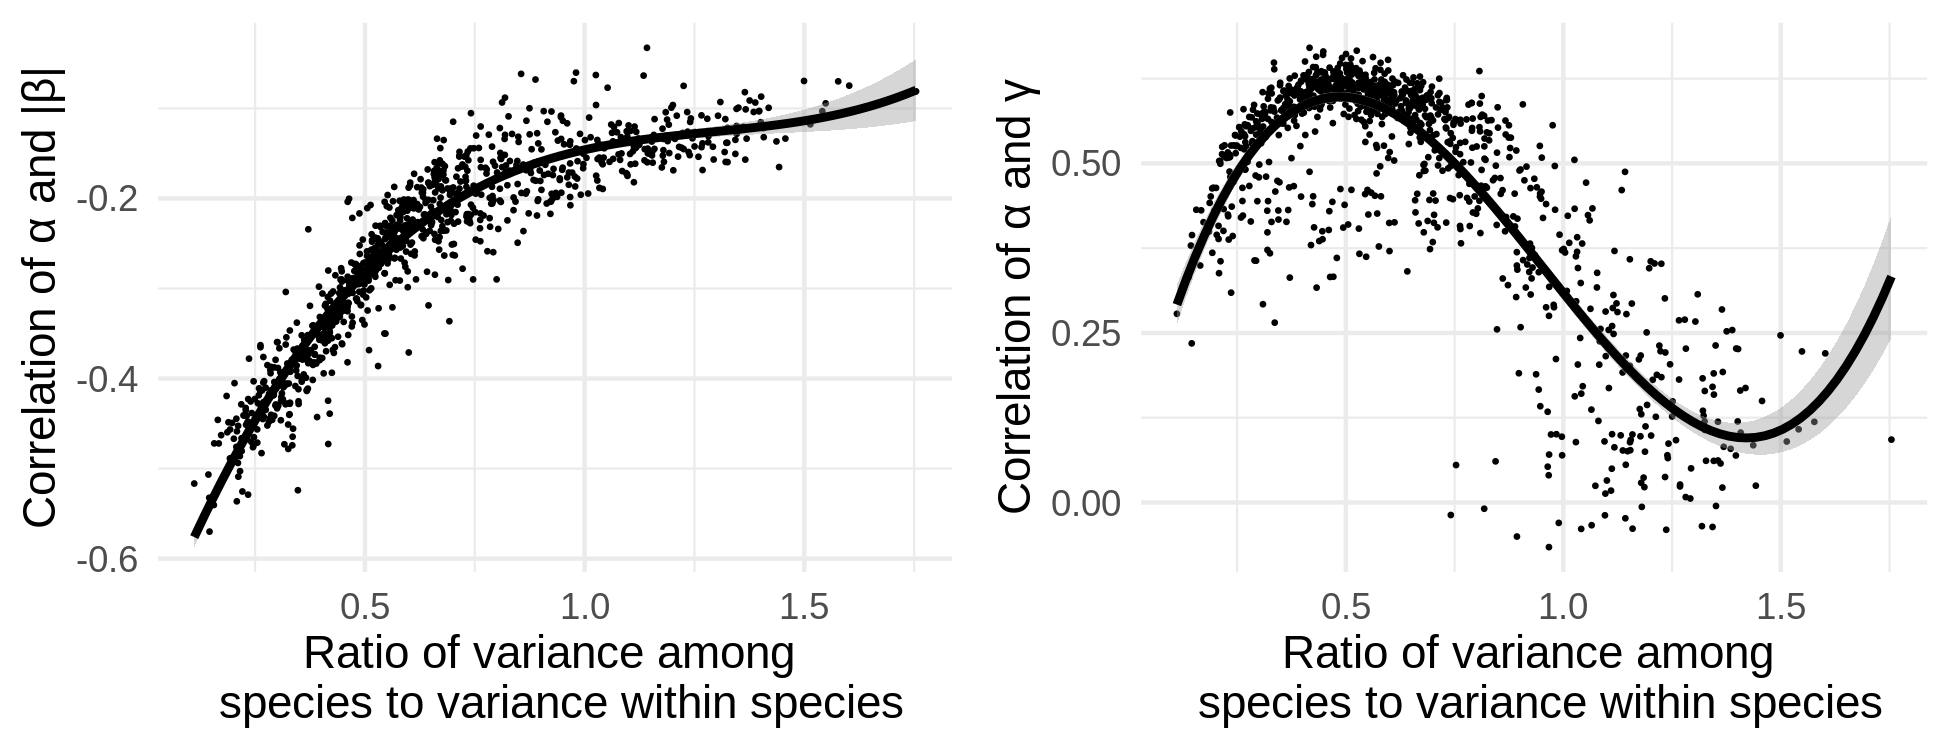
\includegraphics{/home/bb/Gits/branching.brownian.motion.and.spde/.A White Noise Approach To Evolutionary Ecology/corrs} 

}

\caption{Numerical estimate for the correlations of selection gradients and competition coefficients.}\label{fig:unnamed-chunk-13}
\end{figure}

Details on simulations, table of parameters, distributions of \(a\) and
\(c\).

\newpage

\hypertarget{references}{%
\section*{References}\label{references}}
\addcontentsline{toc}{section}{References}

\hypertarget{refs}{}
\leavevmode\hypertarget{ref-AbdalaRoberts2014}{}%
Abdala-Roberts, Luis, and Kailen A. Mooney. 2014. ``Ecological and
Evolutionary Consequences of Plant Genotype Diversity in a Tri-Trophic
System.'' \emph{Ecology} 95 (10). Wiley: 2879--93.

\leavevmode\hypertarget{ref-9781107648258}{}%
Ågren, Göran I., and Folke O. Andersson. 2012. \emph{Terrestrial
Ecosystem Ecology: Principles and Applications}. Cambridge University
Press.

\leavevmode\hypertarget{ref-Barton2017}{}%
Barton, N.H., A.M. Etheridge, and A. Véber. 2017. ``The Infinitesimal
Model: Definition, Derivation, and Implications.'' \emph{Theoretical
Population Biology} 118 (December). Elsevier BV: 50--73.

\leavevmode\hypertarget{ref-Barton2019}{}%
Barton, Nick, and Alison Etheridge. 2019. ``Mathematical Models in
Population Genetics.'' Wiley.

\leavevmode\hypertarget{ref-Barton2013}{}%
Barton, Nick, Alison Etheridge, and Amandine Véber. 2013. ``Modelling
Evolution in a Spatial Continuum.'' \emph{Journal of Statistical
Mechanics: Theory and Experiment} 2013 (01). IOP Publishing: P01002.

\leavevmode\hypertarget{ref-Bertoin2003}{}%
Bertoin, Jean, and Jean-François Le Gall. 2003. ``Stochastic Flows
Associated to Coalescent Processes.'' \emph{Probability Theory and
Related Fields} 126 (2). Springer Science; Business Media: 261--88.

\leavevmode\hypertarget{ref-bulmer1980}{}%
Bulmer. 1980. \emph{The Mathematical Theory of Quantitative Genetics}.
Oxford University Press.

\leavevmode\hypertarget{ref-Brger1986}{}%
Bürger, Reinhard. 1986. ``On the Maintenance of Genetic Variation:
Global Analysis of Kimuras Continuum-of-Alleles Model.'' \emph{Journal
of Mathematical Biology} 24 (3). Springer Nature: 341--51.

\leavevmode\hypertarget{ref-9780471986539}{}%
---------. 2000. \emph{The Mathematical Theory of Selection,
Recombination, and Mutation}. Wiley.

\leavevmode\hypertarget{ref-Cantrell2004}{}%
Cantrell, Robert Stephen, and Chris Cosner. 2004. \emph{Spatial Ecology
via Reaction-Diffusion Equations}. Wiley.

\leavevmode\hypertarget{ref-Case1986}{}%
Case, Ted J., and Mark L. Taper. 1986. ``ON THE COEXISTENCE AND
COEVOLUTION OF ASEXUAL AND SEXUAL COMPETITORS.'' \emph{Evolution} 40
(2). Wiley: 366--87.

\leavevmode\hypertarget{ref-Champagnat2006}{}%
Champagnat, Nicolas, Régis Ferrière, and Sylvie Méléard. 2006.
``Unifying Evolutionary Dynamics: From Individual Stochastic Processes
to Macroscopic Models.'' \emph{Theoretical Population Biology} 69 (3).
Elsevier BV: 297--321.

\leavevmode\hypertarget{ref-Chesson2000}{}%
Chesson, Peter. 2000. ``Mechanisms of Maintenance of Species
Diversity.'' \emph{Annual Review of Ecology and Systematics} 31 (1).
Annual Reviews: 343--66.

\leavevmode\hypertarget{ref-jeffreyconner2004}{}%
Conner, Jeffrey K. 2004. \emph{A Primer of Ecological Genetics}. Sinauer
Associates.

\leavevmode\hypertarget{ref-9781932846126}{}%
Crow, James F., and Motoo Kimura. 1970. \emph{An Introduction to
Population Genetics Theory}. The Blackburn Press.

\leavevmode\hypertarget{ref-Crutsinger2015}{}%
Crutsinger, Gregory M. 2015. ``A Community Genetics Perspective:
Opportunities for the Coming Decade.'' \emph{New Phytologist} 210 (1).
Wiley: 65--70.

\leavevmode\hypertarget{ref-DaPrato2014}{}%
Da Prato, Giuseppe, and Jerzy Zabczyk. 2014. \emph{Stochastic Equations
in Infinite Dimensions}. Cambridge University Press.

\leavevmode\hypertarget{ref-David2019}{}%
David, Thomas I., Jonathan Storkey, and Carly J. Stevens. 2019.
``Understanding How Changing Soil Nitrogen Affects Plantpollinator
Interactions.'' \emph{Arthropod-Plant Interactions} 13 (5). Springer
Science; Business Media LLC: 671--84.

\leavevmode\hypertarget{ref-Dawson1975}{}%
Dawson, Donald A. 1975. ``Stochastic Evolution Equations and Related
Measure Processes.'' \emph{Journal of Multivariate Analysis} 5 (1).
Elsevier BV: 1--52.

\leavevmode\hypertarget{ref-Dawson1978}{}%
---------. 1978. ``Geostochastic Calculus.'' \emph{Canadian Journal of
Statistics} 6 (2). Wiley: 143--68.

\leavevmode\hypertarget{ref-dawson1993measure}{}%
---------. 1993. ``Measure-Valued Markov Processes.'' In \emph{École
d'été de Probabilités de Saint-Flour Xxi-1991}, 1--260. Springer.

\leavevmode\hypertarget{ref-Dbarre2015EvolutionOQ}{}%
Débarre, Florence, Sam Yeaman, and Frédéric Guillaume. 2015. ``Evolution
of Quantitative Traits Under a Migration-Selection Balance: When Does
Skew Matter?'' \emph{The American Naturalist} 186 Suppl 1: S37--47.

\leavevmode\hypertarget{ref-Doebeli1996}{}%
Doebeli, Michael. 1996. ``Quantitative Genetics and Population
Dynamics.'' \emph{Evolution} 50 (2). Wiley: 532--46.

\leavevmode\hypertarget{ref-Engen2013}{}%
Engen, Steinar, Russell Lande, and Bernt-Erik Sæther. 2013. ``A
Quantitative Genetic Model of R- and K-Selection in a Fluctuating
Population.'' \emph{The American Naturalist} 181 (6). University of
Chicago Press: 725--36.

\leavevmode\hypertarget{ref-alisonetheridge2000}{}%
Etheridge, Alison M. 2000. \emph{An Introduction to Superprocesses}.
American Mathematical Society.

\leavevmode\hypertarget{ref-Etheridge2008}{}%
---------. 2008. ``Drift, Draft and Structure: Some Mathematical Models
of Evolution.'' In \emph{Stochastic Models in Biological Sciences}.
Institute of Mathematics Polish Academy of Sciences.

\leavevmode\hypertarget{ref-Etheridge1991}{}%
Etheridge, Alison, and Peter March. 1991. ``A Note on Superprocesses.''
\emph{Probability Theory and Related Fields} 89 (2). Springer: 141--47.

\leavevmode\hypertarget{ref-lawrenceevans2010}{}%
Evans, Lawrence C. 2010. \emph{Partial Differential Equations: Second
Edition}. American Mathematical Society.

\leavevmode\hypertarget{ref-9781470410544}{}%
---------. 2014. \emph{An Introduction to Stochastic Differential
Equations}. American Mathematical Society.

\leavevmode\hypertarget{ref-Evans1994}{}%
Evans, Steven N., and Edwin A. Perkins. 1994. ``Measure-Valued Branching
Diffusions with Singular Interactions.'' \emph{Canadian Journal of
Mathematics} 46 (1). Canadian Mathematical Society: 120--68.

\leavevmode\hypertarget{ref-Ewens2004}{}%
Ewens, Warren J. 2004. \emph{Mathematical Population Genetics}. Springer
New York.

\leavevmode\hypertarget{ref-kennethfalconer2014}{}%
Falconer, Kenneth. 2014. \emph{Fractal Geometry: Mathematical
Foundations and Applications}. Wiley.

\leavevmode\hypertarget{ref-stanleyfarlow1993}{}%
Farlow, Stanley J. 1993. \emph{Partial Differential Equations for
Scientists and Engineers}. Dover.

\leavevmode\hypertarget{ref-feller1951}{}%
Feller, William. 1951. ``Diffusion Processes in Genetics.'' In
\emph{Proceedings of the Second Berkeley Symposium on Mathematical
Statistics and Probability}, 227--46. University of California Press.

\leavevmode\hypertarget{ref-Felsenstein1975}{}%
Felsenstein, Joseph. 1975. ``A Pain in the Torus: Some Difficulties with
Models of Isolation by Distance.'' \emph{The American Naturalist} 109
(967). University of Chicago Press: 359--68.

\leavevmode\hypertarget{ref-Fisher1923}{}%
Fisher, R. A. 1923. ``XXI.-on the Dominance Ratio.'' \emph{Proceedings
of the Royal Society of Edinburgh} 42. Cambridge University Press:
321--41.

\leavevmode\hypertarget{ref-Fitzpatrick2015}{}%
Fitzpatrick, Connor R., Anurag A. Agrawal, Nathan Basiliko, Amy P.
Hastings, Marney E. Isaac, Michael Preston, and Marc T. J. Johnson.
2015. ``The Importance of Plant Genotype and Contemporary Evolution for
Terrestrial Ecosystem Processes.'' \emph{Ecology} 96 (10). Wiley:
2632--42.

\leavevmode\hypertarget{ref-Fitzpatrick2017}{}%
Fitzpatrick, Connor R., Anna V. Mikhailitchenko, Daniel N. Anstett, and
Marc T. J. Johnson. 2017. ``The Influence of Range-Wide Plant Genetic
Variation on Soil Invertebrate Communities.'' \emph{Ecography} 41 (7).
Wiley: 1135--46.

\leavevmode\hypertarget{ref-FRANK2012}{}%
Frank, S. A. 2012. ``Natural Selection. IV. The Price Equation.''
\emph{Journal of Evolutionary Biology} 25 (6). Wiley: 1002--19.

\leavevmode\hypertarget{ref-Fridley2017}{}%
Fridley, Jason D. 2017. ``Plant Energetics and the Synthesis of
Population and Ecosystem Ecology.'' Edited by David Gibson.
\emph{Journal of Ecology} 105 (1). Wiley: 95--110.

\leavevmode\hypertarget{ref-FUSSMANN2007}{}%
Fussman, G. F., M. Loreau, and P. A. Abrams. 2007. ``Eco-Evolutionary
Dynamics of Communities and Ecosystems.'' \emph{Functional Ecology} 21
(3). Wiley: 465--77.

\leavevmode\hypertarget{ref-Gomulkiewicz2017}{}%
Gomulkiewicz, Richard, Stephen M. Krone, and Christopher H. Remien.
2017. ``Evolution and the Duration of a Doomed Population.''
\emph{Evolutionary Applications} 10 (5). Wiley: 471--84.

\leavevmode\hypertarget{ref-Harmon2019}{}%
Harmon, Luke J., Cecilia S. Andreazzi, Florence Débarre, Jonathan Drury,
Emma E. Goldberg, Ayana B. Martins, Carlos J. Melián, et al. 2019.
``Detecting the Macroevolutionary Signal of Species Interactions.''
\emph{Journal of Evolutionary Biology} 32 (8). Wiley: 769--82.

\leavevmode\hypertarget{ref-Harte2011}{}%
Harte, John. 2011. \emph{Maximum Entropy and Ecology}. Oxford University
Press.

\leavevmode\hypertarget{ref-Harte2014}{}%
Harte, John, and Erica A. Newman. 2014. ``Maximum Information Entropy: A
Foundation for Ecological Theory.'' \emph{Trends in Ecology \&
Evolution} 29 (7). Elsevier BV: 384--89.

\leavevmode\hypertarget{ref-Hickerson2010}{}%
Hickerson, M.J., B.C. Carstens, J. Cavender-Bares, K.A. Crandall, C.H.
Graham, J.B. Johnson, L. Rissler, P.F. Victoriano, and A.D. Yoder. 2010.
``Phylogeography's Past, Present, and Future: 10 Years After Avise,
2000.'' \emph{Molecular Phylogenetics and Evolution} 54 (1). Elsevier
BV: 291--301.

\leavevmode\hypertarget{ref-Hofbauer1998}{}%
Hofbauer, Josef, and Karl Sigmund. 1998. \emph{Evolutionary Games and
Population Dynamics}. Cambridge University Press.

\leavevmode\hypertarget{ref-Holt1987}{}%
Holt, Robert D. 1987. ``On the Relation Between Niche Overlap and
Competition: The Effect of Incommensurable Niche Dimensions.''
\emph{Oikos} 48 (1). JSTOR: 110.

\leavevmode\hypertarget{ref-Johnson2005}{}%
Johnson, Toby, and Nick Barton. 2005. ``Theoretical Models of Selection
and Mutation on Quantitative Traits.'' \emph{Philosophical Transactions
of the Royal Society B: Biological Sciences} 360 (1459). The Royal
Society: 1411--25.

\leavevmode\hypertarget{ref-Kendall1966}{}%
Kendall, David G. 1966. ``Branching Processes Since 1873.''
\emph{Journal of the London Mathematical Society} s1-41 (1). Wiley:
385--406.

\leavevmode\hypertarget{ref-Kimmel2015}{}%
Kimmel, Marek, and David E. Axelrod. 2015. \emph{Branching Processes in
Biology}. Springer New York.

\leavevmode\hypertarget{ref-Kimura1965}{}%
Kimura, M. 1965. ``A Stochastic Model Concerning the Maintenance of
Genetic Variability in Quantitative Characters.'' \emph{Proceedings of
the National Academy of Sciences} 54 (3). Proceedings of the National
Academy of Sciences: 731--36.

\leavevmode\hypertarget{ref-Kimura1978}{}%
Kimura, M., and J. F. Crow. 1978. ``Effect of Overall Phenotypic
Selection on Genetic Change at Individual Loci.'' \emph{Proceedings of
the National Academy of Sciences} 75 (12). Proceedings of the National
Academy of Sciences: 6168--71.

\leavevmode\hypertarget{ref-Kirkpatrick1727}{}%
Kirkpatrick, Mark, Toby Johnson, and Nick Barton. 2002. ``General Models
of Multilocus Evolution.'' \emph{Genetics} 161 (4). Genetics: 1727--50.

\leavevmode\hypertarget{ref-kolmogorov1999elements}{}%
Kolmogorov, A.N., and S.V. Fomin. 1999. \emph{Elements of the Theory of
Functions and Functional Analysis}. v. 1. Dover.

\leavevmode\hypertarget{ref-Konno1988}{}%
Konno, N., and T. Shiga. 1988. ``Stochastic Partial Differential
Equations for Some Measure-Valued Diffusions.'' \emph{Probability Theory
and Related Fields} 79 (2). Springer Nature: 201--25.

\leavevmode\hypertarget{ref-Kopp2006}{}%
Kopp, Michael, and Sergey Gavrilets. 2006. ``Multilocus Gentics and the
Coevolution of Quantitative Traits.'' \emph{Evolution} 60 (7). Wiley:
1321--36.

\leavevmode\hypertarget{ref-Klzsch2015}{}%
Kölzsch, Andrea, Adriana Alzate, Frederic Bartumeus, Monique de Jager,
Ellen J. Weerman, Geerten M. Hengeveld, Marc Naguib, Bart A. Nolet, and
Johan van de Koppel. 2015. ``Experimental Evidence for Inherent Lévy
Search Behaviour in Foraging Animals.'' \emph{Proceedings of the Royal
Society B: Biological Sciences} 282 (1807). The Royal Society: 20150424.

\leavevmode\hypertarget{ref-Kraft2007}{}%
Kraft, Nathan J. B., William K. Cornwell, Campbell O. Webb, and David D.
Ackerly. 2007. ``Trait Evolution, Community Assembly, and the
Phylogenetic Structure of Ecological Communities.'' \emph{The American
Naturalist} 170 (2). University of Chicago Press: 271--83.

\leavevmode\hypertarget{ref-Krylov1981}{}%
Krylov, N. V., and B. L. Rozovskii. 1981. ``Stochastic Evolution
Equations.'' \emph{Journal of Soviet Mathematics} 16 (4). Springer
Science; Business Media LLC: 1233--77.

\leavevmode\hypertarget{ref-Lande1975}{}%
Lande, Russell. 1975. ``The Maintenance of Genetic Variability by
Mutation in a Polygenic Character with Linked Loci.'' \emph{Genetical
Research} 26 (3). Cambridge University Press (CUP): 221--35.

\leavevmode\hypertarget{ref-Lande1976}{}%
---------. 1976. ``Natural Selection and Random Genetic Drift in
Phenotypic Evolution.'' \emph{Evolution} 30 (2). Wiley: 314--34.

\leavevmode\hypertarget{ref-pmid17248993}{}%
---------. 1980. ``The Genetic Covariance between Characters Maintained
by Pleiotropic Mutations.'' \emph{Genetics} 94 (1): 203--15.

\leavevmode\hypertarget{ref-Lande1982}{}%
---------. 1982. ``A Quantitative Genetic Theory of Life History
Evolution.'' \emph{Ecology} 63 (3). Wiley: 607--15.

\leavevmode\hypertarget{ref-Lande1995}{}%
---------. 1995. ``Mutation and Conservation.'' \emph{Conservation
Biology} 9 (4). Wiley: 782--91.

\leavevmode\hypertarget{ref-Lande1983}{}%
Lande, Russell, and Stevan J. Arnold. 1983. ``The Measurement of
Selection on Correlated Characters.'' \emph{Evolution} 37 (6). JSTOR:
1210.

\leavevmode\hypertarget{ref-Lande2003}{}%
Lande, Russell, Steinar Engen, and Bernt-Erik SÆther. 2003.
``Demographic and Environmental Stochasticity.'' In \emph{Stochastic
Population Dynamics in Ecology and Conservation}, 1--24. Oxford
University Press.

\leavevmode\hypertarget{ref-Lande2009}{}%
Lande, Russell, Steinar Engen, and Bernt-Erik Sæther. 2009. ``An
Evolutionary Maximum Principle for Density-Dependent Population Dynamics
in a Fluctuating Environment.'' \emph{Philosophical Transactions of the
Royal Society B: Biological Sciences} 364 (1523). The Royal Society:
1511--8.

\leavevmode\hypertarget{ref-Landis2017}{}%
Landis, Michael J., and Joshua G. Schraiber. 2017. ``Pulsed Evolution
Shaped Modern Vertebrate Body Sizes.'' \emph{Proceedings of the National
Academy of Sciences} 114 (50). Proceedings of the National Academy of
Sciences: 13224--9.

\leavevmode\hypertarget{ref-9780691080628}{}%
Levins, Richard. 1968. \emph{Evolution in Changing Environments: Some
Theoretical Explorations. (MPB-2) (Monographs in Population Biology)}.
Princeton University Press.

\leavevmode\hypertarget{ref-zeng1998absolute}{}%
Li, Zeng-Hu. 1998. ``Absolute Continuity of Measure Branching Processes
with Interaction.'' \emph{Chinese Journal of Applied Probability and
Statistics} 14. Citeseer: 231--42.

\leavevmode\hypertarget{ref-Lion2018}{}%
Lion, Sébastien. 2018. ``Theoretical Approaches in Evolutionary Ecology:
Environmental Feedback as a Unifying Perspective.'' \emph{The American
Naturalist} 191 (1). University of Chicago Press: 21--44.

\leavevmode\hypertarget{ref-michelloreau2010}{}%
Loreau, Michel. 2010. \emph{From Populations to Ecosystems: Theoretical
Foundations for a New Ecological Synthesis}. Princeton University Press.

\leavevmode\hypertarget{ref-michaellynch1998}{}%
Lynch, Michael, and Bruce Walsh. 1998. \emph{Genetics and Analysis of
Quantitative Traits}. Sinauer Associates is an imprint of Oxford
University Press.

\leavevmode\hypertarget{ref-Arthur1969}{}%
MacArthur, Robert H. 1969. ``Species Packing, and what Competition
Minimizes.'' \emph{Proceedings of the National Academy of Sciences} 64
(4). Proceedings of the National Academy of Sciences: 1369--71.

\leavevmode\hypertarget{ref-MacArthur1970}{}%
---------. 1970. ``Species Packing and Competitive Equilibrium for Many
Species.'' \emph{Theoretical Population Biology} 1 (1). Elsevier BV:
1--11.

\leavevmode\hypertarget{ref-9780691023823}{}%
---------. 1972. \emph{Geographical Ecology}. Princeton University
Press.

\leavevmode\hypertarget{ref-Macarthur1967}{}%
MacArthur, Robert H., and Richard Levins. 1967. ``The Limiting
Similarity, Convergence, and Divergence of Coexisting Species.''
\emph{The American Naturalist} 101 (921). University of Chicago Press:
377--85.

\leavevmode\hypertarget{ref-Manceau2016}{}%
Manceau, Marc, Amaury Lambert, and Hélène Morlon. 2016. ``A Unifying
Comparative Phylogenetic Framework Including Traits Coevolving Across
Interacting Lineages.'' \emph{Systematic Biology}, December. Oxford
University Press (OUP), syw115.

\leavevmode\hypertarget{ref-Marx2017}{}%
Marx, Hannah E., Cédric Dentant, Julien Renaud, Romain Delunel, David C.
Tank, and Sébastien Lavergne. 2017. ``Riders in the Sky (Islands): Using
a Mega-Phylogenetic Approach to Understand Plant Species Distribution
and Coexistence at the Altitudinal Limits of Angiosperm Plant Life.''
\emph{Journal of Biogeography} 44 (11). Wiley: 2618--30.

\leavevmode\hypertarget{ref-markmcpeek2017}{}%
McPeek, Mark A. 2017. \emph{Evolutionary Community Ecology}. Princeton
University Press.

\leavevmode\hypertarget{ref-DeMeester2018}{}%
Meester, Luc De, Kristien I. Brans, Lynn Govaert, Caroline Souffreau,
Shinjini Mukherjee, Héléne Vanvelk, Konrad Korzeniowski, et al. 2018.
``Analyzing Eco-Evolutionary Dynamics - the Challenging Complexity of
the Real World.'' \emph{Functional Ecology}. Wiley.

\leavevmode\hypertarget{ref-meleard1992interacting}{}%
Méléard, M, and S Roelly. 1992. ``Interacting Branching Measure
Processes.'' \emph{Stochastic Partial Differential Equations and
Applications (G. Da Prato and L. Tubaro, Eds.)}, 246--56.

\leavevmode\hypertarget{ref-Mlard1993}{}%
---------. 1993. ``Interacting Measure Branching Processes. Some Bounds
for the Support.'' \emph{Stochastics and Stochastic Reports} 44 (1-2).
Informa UK Limited: 103--21.

\leavevmode\hypertarget{ref-Mubayi2019}{}%
Mubayi, Anuj, Christopher Kribs, Viswanathan Arunachalam, and Carlos
Castillo-Chavez. 2019. ``Studying Complexity and Risk Through Stochastic
Population Dynamics: Persistence, Resonance, and Extinction in
Ecosystems.'' In \emph{Handbook of Statistics}, 157--93. Elsevier.

\leavevmode\hypertarget{ref-9780674023383}{}%
Nowak, Martin A. 2006. \emph{Evolutionary Dynamics: Exploring the
Equations of Life}. Belknap Press.

\leavevmode\hypertarget{ref-Nuismer2005}{}%
Nuismer, Scott L., Michael Doebeli, and Danny Browning. 2005. ``The
Coevolutionary Dynamics of Antagonistic Interactions Mediated by
Quantitative Traits with Evolving Variances.'' \emph{Evolution} 59 (10).
The Society for the Study of Evolution: 2073.

\leavevmode\hypertarget{ref-Nuismer2014}{}%
Nuismer, Scott L., and Luke J. Harmon. 2014. ``Predicting Rates of
Interspecific Interaction from Phylogenetic Trees.'' Edited by Jerome
Chave. \emph{Ecology Letters} 18 (1). Wiley: 17--27.

\leavevmode\hypertarget{ref-Nuismer2012}{}%
Nuismer, Scott L., Pedro Jordano, and Jordi Bascompte. 2012.
``Coevolution and the Architecture of Mutualistic Networks.''
\emph{Evolution} 67 (2). Wiley: 338--54.

\leavevmode\hypertarget{ref-Nuismer2007}{}%
Nuismer, Scott L., Benjamin J. Ridenhour, and Benjamin P. Oswald. 2007.
``Antagonistic Coevolution Mediated by Phenotypic Differenes Between
Quantitative Traits.'' \emph{Evolution} 61 (8). Wiley: 1823--34.

\leavevmode\hypertarget{ref-Nuismer2018}{}%
Nuismer, Scott L., Bob Week, and Marcelo A. Aizen. 2018. ``Coevolution
Slows the Disassembly of Mutualistic Networks.'' \emph{The American
Naturalist} 192 (4). University of Chicago Press: 490--502.

\leavevmode\hypertarget{ref-VanNuland2019}{}%
Nuland, Michael E. Van, Ian M. Ware, Joseph K. Bailey, and Jennifer A.
Schweitzer. 2019. ``Ecosystem Feedbacks Contribute to Geographic
Variation in Plant-Soil Eco-Evolutionary Dynamics Across a Fertility
Gradient.'' Edited by Franziska Brunner. \emph{Functional Ecology} 33
(1). Wiley: 95--106.

\leavevmode\hypertarget{ref-PAGE2002}{}%
Page, Karen M., and Martin A. Nowak. 2002. ``Unifying Evolutionary
Dynamics.'' \emph{Journal of Theoretical Biology} 219 (1). Elsevier BV:
93--98.

\leavevmode\hypertarget{ref-Parachnowitsch2018}{}%
Parachnowitsch, Amy L, Jessamyn S Manson, and Nina Sletvold. 2018.
``Evolutionary Ecology of Nectar.'' \emph{Annals of Botany} 123 (2).
Oxford University Press (OUP): 247--61.

\leavevmode\hypertarget{ref-Park2017}{}%
Park, Briton, Matthew T. Rutter, Charles B. Fenster, V. Vaughan Symonds,
Mark C. Ungerer, and Jeffrey P. Townsend. 2017. ``Distributions of
Mutational Effects and the Estimation of Directional Selection in
Divergent Lineages ofArabidopsis Thaliana.'' \emph{Genetics} 206 (4).
Genetics Society of America: 2105--17.

\leavevmode\hypertarget{ref-Parsons2010}{}%
Parsons, Todd L., Christopher Quince, and Joshua B. Plotkin. 2010.
``Some Consequences of Demographic Stochasticity in Population
Genetics.'' \emph{Genetics} 185 (4). Genetics Society of America:
1345--54.

\leavevmode\hypertarget{ref-Patel2019}{}%
Patel, Swati, and Reinhard Bürger. 2019. ``Eco-Evolutionary Feedbacks
Between Prey Densities and Linkage Disequilibrium in the Predator
Maintain Diversity.'' \emph{Evolution} 73 (8). Wiley: 1533--48.

\leavevmode\hypertarget{ref-Perkins1991}{}%
Perkins, Edwin A. 1991. ``Conditional Dawson-Watanabe Processes and
Fleming-Viot Processes.'' In \emph{Seminar on Stochastic Processes,
1991}, 143--56. Birkhäuser Boston.

\leavevmode\hypertarget{ref-Perkins1992}{}%
---------. 1992. ``Measure-Valued Branching Diffusions with Spatial
Interactions.'' \emph{Probability Theory and Related Fields} 94 (2).
Springer Science; Business Media LLC: 189--245.

\leavevmode\hypertarget{ref-edwinarendperkins1995}{}%
---------. 1995. \emph{On the Martingale Problem for Interactive
Measure-Valued Branching Diffusions}. Amer Mathematical Society.

\leavevmode\hypertarget{ref-PRICE1970}{}%
Price, George R. 1970. ``Selection and Covariance.'' \emph{Nature} 227
(5257). Springer Nature: 520--21.

\leavevmode\hypertarget{ref-Queller2017}{}%
Queller, David C. 2017. ``Fundamental Theorems of Evolution.'' \emph{The
American Naturalist} 189 (4). University of Chicago Press: 345--53.

\leavevmode\hypertarget{ref-Reimers1989}{}%
Reimers, Mark. 1989. ``One Dimensional Stochastic Partial Differential
Equations and the Branching Measure Diffusion.'' \emph{Probability
Theory and Related Fields} 81 (3). Springer Nature: 319--40.

\leavevmode\hypertarget{ref-Robertson1966}{}%
Robertson, Alan. 1966. ``A Mathematical Model of the Culling Process in
Dairy Cattle.'' \emph{Animal Science} 8 (1). Cambridge University Press:
95--108.

\leavevmode\hypertarget{ref-joanroughgarden1979}{}%
Roughgarden, Joan. 1979. \emph{Theory of Population Genetics and
Evolutionary Ecology: An Introduction}. Macmillan.

\leavevmode\hypertarget{ref-Rudman2017}{}%
Rudman, Seth M., Matthew A. Barbour, Katalin Csilléry, Phillip Gienapp,
Frederic Guillaume, Nelson G. Hairston Jr, Andrew P. Hendry, et al.
2017. ``What Genomic Data Can Reveal About Eco-Evolutionary Dynamics.''
\emph{Nature Ecology \& Evolution} 2 (1). Springer Nature: 9--15.

\leavevmode\hypertarget{ref-Schreiber2017}{}%
Schreiber, Sebastian J. 2017. ``Coexistence in the Face of
Uncertainty.'' In \emph{Recent Progress and Modern Challenges in Applied
Mathematics, Modeling and Computational Science}, 349--84. Springer New
York.

\leavevmode\hypertarget{ref-Schreiber2018}{}%
Schreiber, Sebastian J., Swati Patel, and Casey terHorst. 2018.
``Evolution as a Coexistence Mechanism: Does Genetic Architecture
Matter?'' \emph{The American Naturalist} 191 (3). University of Chicago
Press: 407--20.

\leavevmode\hypertarget{ref-Schuster1983}{}%
Schuster, Peter, and Karl Sigmund. 1983. ``Replicator Dynamics.''
\emph{Journal of Theoretical Biology} 100 (3). Elsevier BV: 533--38.

\leavevmode\hypertarget{ref-Skovmand2018}{}%
Skovmand, Lotte H., Charles C.Y. Xu, Maria R. Servedio, Patrik Nosil,
Rowan D.H. Barrett, and Andrew P. Hendry. 2018. ``Keystone Genes.''
\emph{Trends in Ecology \& Evolution} 33 (9). Elsevier BV: 689--700.

\leavevmode\hypertarget{ref-Sterner2008}{}%
Sterner, R.W., and J.J. Elser. 2008. ``Ecological Stoichiometry:
Overview.'' In \emph{Encyclopedia of Ecology}, 1101--16. Elsevier.

\leavevmode\hypertarget{ref-Taylor1978}{}%
Taylor, Peter D., and Leo B. Jonker. 1978. ``Evolutionary Stable
Strategies and Game Dynamics.'' \emph{Mathematical Biosciences} 40
(1-2). Elsevier BV: 145--56.

\leavevmode\hypertarget{ref-davidtilman1982}{}%
Tilman, David. 1982. \emph{Resource Competition and Community
Structure}. Princeton University Press.

\leavevmode\hypertarget{ref-Turelli1980}{}%
Turelli, Michael. 1980. ``Niche Overlap and Invasion of Competitors in
Random Environments II. The Effects of Demographic Stochasticity.'' In
\emph{Biological Growth and Spread}, 119--29. Springer Berlin
Heidelberg.

\leavevmode\hypertarget{ref-Turelli1984}{}%
---------. 1984. ``Heritable Genetic Variation via Mutation-Selection
Balance: Lerchs Zeta Meets the Abdominal Bristle.'' \emph{Theoretical
Population Biology} 25 (2). Elsevier: 138--93.

\leavevmode\hypertarget{ref-Turelli1986}{}%
---------. 1986. ``Gaussian Versus Non-Gaussian Genetic Analyses of
Polygenic Mutation-Selection Balance.'' In \emph{Evolutionary Processes
and Theory}, 607--28. Academic Press.

\leavevmode\hypertarget{ref-Turelli2017}{}%
---------. 2017. ``Commentary: Fisher's Infinitesimal Model: A Story for
the Ages.'' \emph{Theoretical Population Biology} 118 (December).
Elsevier BV: 46--49.

\leavevmode\hypertarget{ref-pmid7851785}{}%
Turelli, Michael, and Nick Barton. 1994. ``Genetic and statistical
analyses of strong selection on polygenic traits: what, me normal?''
\emph{Genetics} 138 (3): 913--41.

\leavevmode\hypertarget{ref-Volpert2014}{}%
Volpert, Vitaly. 2014. \emph{Elliptic Partial Differential Equations:
Volume 2: Reaction-Diffusion Equations}. Springer Basel.

\leavevmode\hypertarget{ref-Walsh}{}%
Walsh, John B. 1986. ``An Introduction to Stochastic Partial
Differential Equations.'' In \emph{Lecture Notes in Mathematics},
265--439. Springer Berlin Heidelberg.

\leavevmode\hypertarget{ref-Watanabe1968}{}%
Watanabe, Shinzo. 1968. ``A Limit Theorem of Branching Processes and
Continuous State Branching Processes.'' \emph{Journal of Mathematics of
Kyoto University} 8 (1). Duke University Press: 141--67.

\leavevmode\hypertarget{ref-Wright97}{}%
Wright, Sewall. 1931. ``Evolution in Mendelian Populations.''
\emph{Genetics} 16 (2). Genetics: 97--159.

\leavevmode\hypertarget{ref-Xiao2015}{}%
Xiao, Xiao, Daniel J. McGlinn, and Ethan P. White. 2015. ``A Strong Test
of the Maximum Entropy Theory of Ecology.'' \emph{The American
Naturalist} 185 (3). University of Chicago Press: E70--E80.

\leavevmode\hypertarget{ref-zheng2004nonlinear}{}%
Zheng, Songmu. 2004. \emph{Nonlinear Evolution Equations}. Boca Raton,
Fla: Chapman \& Hall/CRC Press.

\end{document}
